\chapter{Experiments, Results and Analysis}\label{chap:experiments_and_results}

% Present the chapter
In this Chapter, the results are presented and a rigorous
analysis is realized. In Section~\ref{sec:design_of_experiments}
the design of experiments is presented, where the outlines of how
and where the experiments were executed is explained. The methodology
for comparison is also discussed in that section. In
Section~\ref{sec:methods-analysis} a rigorous set of statistical
tests is presented and applied to the results, with the goal of
comparing the proposed methods against references in the literature.
The genotipic and fenotipic diversity of the two proposed method is
inspected and analysed in~\ref{sec:convergence-analysis}.
An analysis of the two proposed methods is presented in
Section~\ref{sec:methods-duel}, where it is verified if there is one with a
superior performance and which one.
In Section~\ref{sec:repacking-impact} an analysis of the impact that
repacking has on the proposed methods is presented. This, compares how
the RMSD and energy, relative to rosetta, changed when repacking was
applied. This section has two goals. First, to identify if repacking
did or did not influence the results from the statistical tests.
Secondly, to document its impact.

The processing time required to run the proposed methods is exposed in
Section~\ref{sec:time-and-evals}, along with the number of spent function
evaluations. Then, in Section~\ref{sec:competing-methods} an in depth
analysis of the two proposed methods is presented, where they are
compared versus more than 20 works in the literature.
Section~\ref{sec:other-metrics} presents an analysis using GDT-TS
and TM-Score, with the aim of providing further insight on the results.
Furthermore, the raw data from the experiments is also provided with
the object of allowing further works to more easily compare with the
presented methods. A visual analysis of the best conformations is
presented in Section~\ref{sec:visual-analysis}, where some of the
prediction problems can be identified and are commented.

\section{Design of Experiments}\label{sec:design_of_experiments}

% Present the hardware setup
The experiments were all conducted on a single machine using the same hardware
throughout the full experimentation. Table~\ref{tab:machine-setup}
presents the machine utilized to run all the experiments. Each run of a
prediction method consists of a serial program that run continually without
interruption. The experiments were run in parallel, limited to at most one
running test per core\footnote{Only physical cores were considered. No virtual
(Hyper-threading) core was involved in the computations.}. To ensure maximum
repeatability the machine had no graphical interface enabled or any other form
of user interaction during the course of the experimentation.

\begin{table}[th]
    \centering
    \begin{tabular}{r|l} \hline \hline
        Name & Value \\ \hline \hline
        Operating System & Arch Linux \\ \hline
        Kernel &  Arch Linux Kernel 4.18.16 \\ \hline
        CPU & Intel(R) Core(TM) i5-3570K CPU @ 4.20GHz \\ \hline
        Number of Cores & 4 Physical cores, no hyper-threading cores \\ \hline
        RAM & 16 GB @ 1400 MHz \\ \hline \hline
    \end{tabular}
    \caption{The Machine Setup}
    \label{tab:machine-setup}
\end{table}

The experimentation consisted of running the two proposed methods, namely
PPF-REMCc and PPF-MC. One of the methods proposed
in~\cite{silva2019self} is also included, namely SADE-REMC.
Lastly, the Rosetta Ab Initio protocol is also included, amounting to four
different methods being ran.

The analysis is divided in two steps. In the first one, the two proposed methods
are compared against the work from~\citeonline{silva2019self} and the Rosetta Ab Initio
Protocol.
\textcolor{red}{Rosetta was selected as an representative of the state of art,
while the other method, SADE-REMC, is a precursor of the two proposed methods.
Since there is open
access to both methods, it is possible to run and analyze experiments with them
more easily and to do a direct statistical analyse on the results.
}

% Present the "in house" comparison
The metrics utilized are the \textit{scorefxn} energy value of the
best solution and the \ac{RMSD} associated with the this conformation. The
results were collected over 50 independent runs of each method for each target
protein. A graphical analysis is conducted in order to identify visually the
relative performance between the proposed methods. Considering that a visual
analysis is not enough (in this case), a more rigorous numerical statistic set
of test is conducted. The Shapiro-Wilk~\cite{wilk1968joint} normality test is
employed with a confidence level of 5\%, i.e. $\alpha = 0.05$, to assess the
presence (or lack) of an underlying normal distribution. Based on its result, a
parametric/non-parametric test is employed with a confidence level of $\alpha =
0.05$. Due the presence of multiple comparisons, the Kruskal-Wallis test is
applied in order to detect if there is any method with a performance that
is different than the others. If there is, then, the pairwise Mann-Whitney test is
employed with the proposed methods against its competitors.

% Explain the clustering results
\textcolor{red}{
The use of clustering to extract and return different conformations from the
proposed methods is highly important in a complex and extremely multi-modal
problem such as the PSPP. With clustering, it is possible to identify conformations
that are far apart from each other in the energy landscape, however, that have
similar energies. This process require extra steps during the analysis.}
First, the main use of
returning several conformations is to allow an human expert to choose one that
has the desired properties. This, can not be automated in a test environment where
hundreds of experiments are performed computationally each day. As such, the human
expert, for the purposes of performance evaluation, must be replaced by a
computer oracle. This oracle can always find the conformation with the lowest
RMSD or the conformation with the lowest energy. This, of course, would not
be possible in a real world scenario where a protein without a known structure is
being predicted. With that in mind, the analysis of the two proposed methods is
divided in two sub groups. The first is named \texttt{best-by-rmsd} and the second
is named \texttt{best-by-energy}.

% Present the "free for all" analysis
In the second analysis step, a direct comparison against several works in the
literature is considered. Since there is a severe lack of standardization in the
literature regarding experimentation, the following methodology was used. Works
that provided the best RMSD had their proteins listed. The proteins that occurred
the most were used for comparison. It is worth noting that the majority of works
provide little information about how the experimentation was conducted. The way
in which the results are analysed lacks a standard. As such, this work does a
direct comparison using the best RMSD achieved in a set of runs. While this is
not ideal, due to different works running each method different number of times,
this is possibly the only way to a comparison against several works. %The presence of outliers also weaken this comparison. Also, since only the most used proteins are select, it is possible that some works are only represented partially, i.e. some of the results are left out. 
Nevertheless, at the end of the day for the PSPP what matters is having the lowest possible error. As such, comparing the best RMSD is a worthwhile analysis. %, albeit not ideal.

% Present the protein set
With that in mind, the set of proteins presented in Table~\ref{tab:protein-targets}
was chosen. The column \textbf{Name} contains the protein identification code
as in PDB.  The \textbf{Size} column shows the number of amino acids in the protein.
The \textbf{Backbone Angles} column shows the number of angles in the backbone,
this also has a one to one relation to the number of variables to be optimized
for a given protein. The \textbf{Structure} column holds the secondary
structures present in the protein set represented by $\alpha$-helices or
$\beta$-sheets.

\begin{table}[bh]
  \centering
  \begin{tabular}{ l | c | c | c | c }
    \hline \hline
    Name & Size & Backbone Angles & Structure         \\ \hline \hline
    1l2y & 20   & 60              & $2\alpha$         \\ \hline
    1wqc & 26   & 78              & $2\alpha$         \\ \hline
    1acw & 29   & 87              & $1\alpha, 2\beta$ \\ \hline
    1zdd & 35   & 105             & $2\alpha$         \\ \hline
    2mr9 & 44   & 132             & $3\alpha$         \\ \hline
    1crn & 46   & 138             & $2\alpha, 2\beta$ \\ \hline
    1enh & 54   & 162             & $3\alpha$         \\ \hline
    1rop & 63   & 189             & $2\alpha$         \\ \hline
    1utg & 70   & 210             & $4\alpha$         \\ \hline
    1ail & 72   & 216             & $3\alpha$         \\ \hline
    \hline
  \end{tabular}
  \caption{Target proteins and their features}
  \label{tab:protein-targets}
\end{table}

% Present the parameters
The two proposed methods all operates with the same parameters, as presented
in Table~\ref{tab:parameters}. The first column contains the parameter name and the
second one its respective value.
Population Initialization refers to the \ac{MC} search that is made using
\texttt{score0}. It has $10000$ function evaluations available, such that up to
$100$ are used for each solution vector.
The SaDE learning Phase has its default value,
as presented in~\cite{qin2009differential}. There are 100 simultaneous
trajectories throughout the execution, i.e. a population size of 100. A million
function evaluations are available for the optimization phase, where each
fragment insertion routine can use up to 25 at a time. \ac{FFI} uses a fragment
size of 9 and is applied with a probability of 2\% before each standard fragment
insertion. The other methods being compared use the same values from
Table~\ref{tab:parameters} as applicable.

\begin{table}[ht]
    \centering
    \begin{tabular}{r|l} \hline \hline
        Parameter & Value \\ \hline \hline
        Population Initialization Evaluation Budget & 10000 \\ \hline
        SaDE learning Phase & 50 \\ \hline
        Population Size & 100 \\ \hline
        Function Evaluation Budget & 1000000 \\ \hline
        MC/REMC Function Evaluation Budget & 25 \\ \hline
        Spicker cluster size & 10 \\ \hline
        \ac{FFI} probability & 0.02 \\ \hline
        \ac{FFI} length & 9 \\ \hline \hline
    \end{tabular}
    \caption{Parameters utilized in the proposed methods}
    \label{tab:parameters}
\end{table}

\section{Energy and RMSD Analysis}\label{sec:methods-analysis}

% Introduce the analysis
Due to the amount of data generated by the experiments, most of the analysis will
be conducted by visual inspection or by summarizing the results and key-points.
However, for the sake of completude and scientific rigor, complementary
information is provided in Appendix~\ref{appendix:table-results}.
\textcolor{red}{
Moreover, the analysis is divided in three main parts. In the first part, a visual
analysis using boxplots is used in order to observe the overall performance of
the proposed methods. Following, a statistical framework is used to assess the methods
performance relatively to each other. Then, a pareto front analysis is presented
using the best results from the four methods.
}
% In
% Section~\ref{sec:statistical-analysis} a strictly statistical analysis is
% presented. Section~\ref{sec:pareto-front-analysis} presents an analysis of the
% best results achieved using Pareto Front.

% Present the box plots
In Figure~\ref{fig:boxplot-rmsd} the RMSD from the predictions is presented as box-plots.
The proteins, presented in the x-axis, are displayed in lexicographical order.
The y-axis presents the RMSD, where lower is better. The methods are grouped
horizontally by protein.

It is possible to verify that for 9 out of 10 proteins (with exception for 1rop) the
two proposed methods, in orange and green, had a very close overall performance,
considering the median, presented as the line inside the box of each method.
For 1rop, the ppf-mc outperformed the other methods by a significant margin.
Moreover, the two proposed methods had better medians than
the other methods (not including rosetta) in 8 of the 10 proteins,
with exception for 1rop and 1zdd.
For 1rop, the SADE-REMC had the second best result, behind ppf-mc, while ppf-remc
had the worst result.
For the 1zdd protein, the two proposed methods had the two worst
medians, however, by a relatively small amount.

In a direct comparison against rosetta, proteins 1acw, 1enh, 1l2y, 1utg and 2mr9
the proposed methods had a significant improvement upon rosetta.
\textcolor{red}{
For 1crn the rosetta appears to have had
a slightly better performance compared to the proposed methods.
In the remaining proteins, 1ail, 1rop, 1wqc and 1zdd, it is not
possible to visually detect in a objective manner if there was
a significant performance improve. This, will be address later with statistical
tests.
% visual inspection is not enough to accurately detect significant performance differences.
}

Some other behaviours are worth noting. The manifestation of each
proteins uniqueness is visible in the distribution of different methods. For example,
a simple visual inspection on Figure~\ref{fig:boxplot-rmsd} shows that on
2mr9, rosetta had a worst performance than the other methods by a significant margin,
whereas the other methods had a very similar performance. For 1utg, the two proposed
methods outclassed the other methods, including rosetta. Furthermore, the worst
result from ppf-remc was better than the medians of all the other methods.
Now, interestingly, for 1wqc and 1crn, rosetta and the two proposed methods had
better performance than the other methods. Also, for some proteins, such as 1enh,
the overall performance is much closer. One possible explanation for this difference
in results, considering that all the methods had the same input, is the conformation
sampling strategy. Some strategies might best suit some proteins with a given conformation
structure more than others. All these visual observations are later confirmed with
statistical tests.

\begin{figure}
  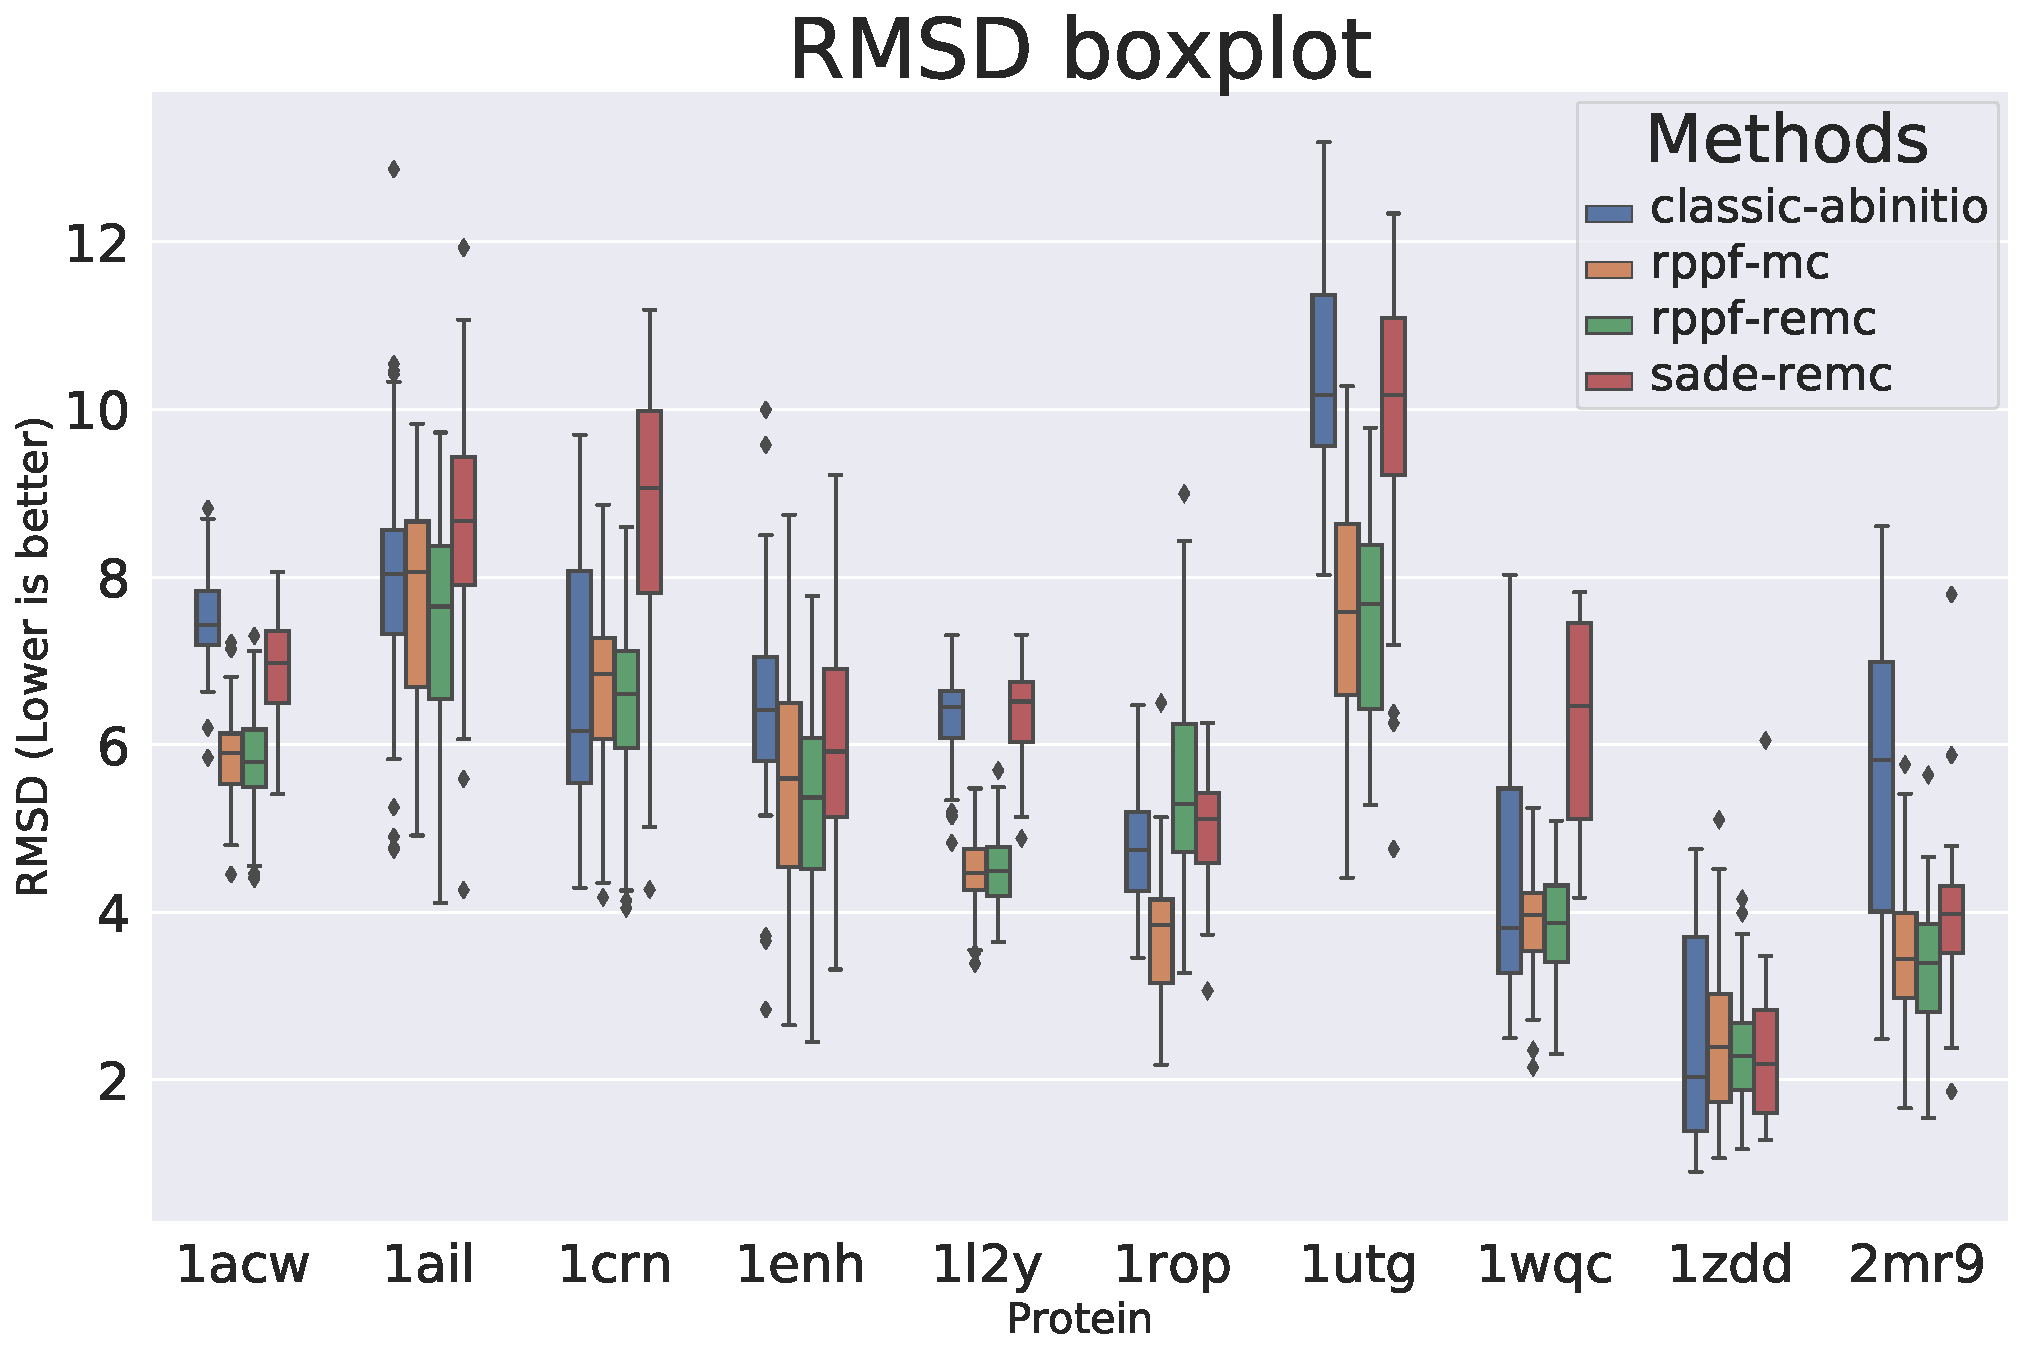
\includegraphics[width=\linewidth]{Figuras/boxplots/boxplot_best_by_rmsd_rmsd_after.pdf}
  \caption{Boxplot presenting the RMSD for the protein predictions with the
    competing methods. For the two proposed methods, the \texttt{best-by-rmsd}
    data was used}
  \label{fig:boxplot-rmsd}
\end{figure}

Figure~\ref{fig:boxplot-energy} presents data similarly to the previous figure,
however, the y-axis now represents the \texttt{scorefxn} energy function. Considering
the energy results, when compared to the rmsd boxplot, the results are relatively
more similar. Nevertheless, for some proteins there are some behaviours that are
more visible. For 1rop, ppf-remc appears to have had a worst performance
than the other methods. Same as with the RMSD data. For 1crn, rosetta and the two
proposed methods appears to have a better overall result. For 2mr9, rosetta
appears to be lagging behind in performance. These observations are just visual
trends which helps understand the relative performance.
% In order to properly
% access their differences a more rigorous statistical approach is required and exposed next.

\begin{figure}
  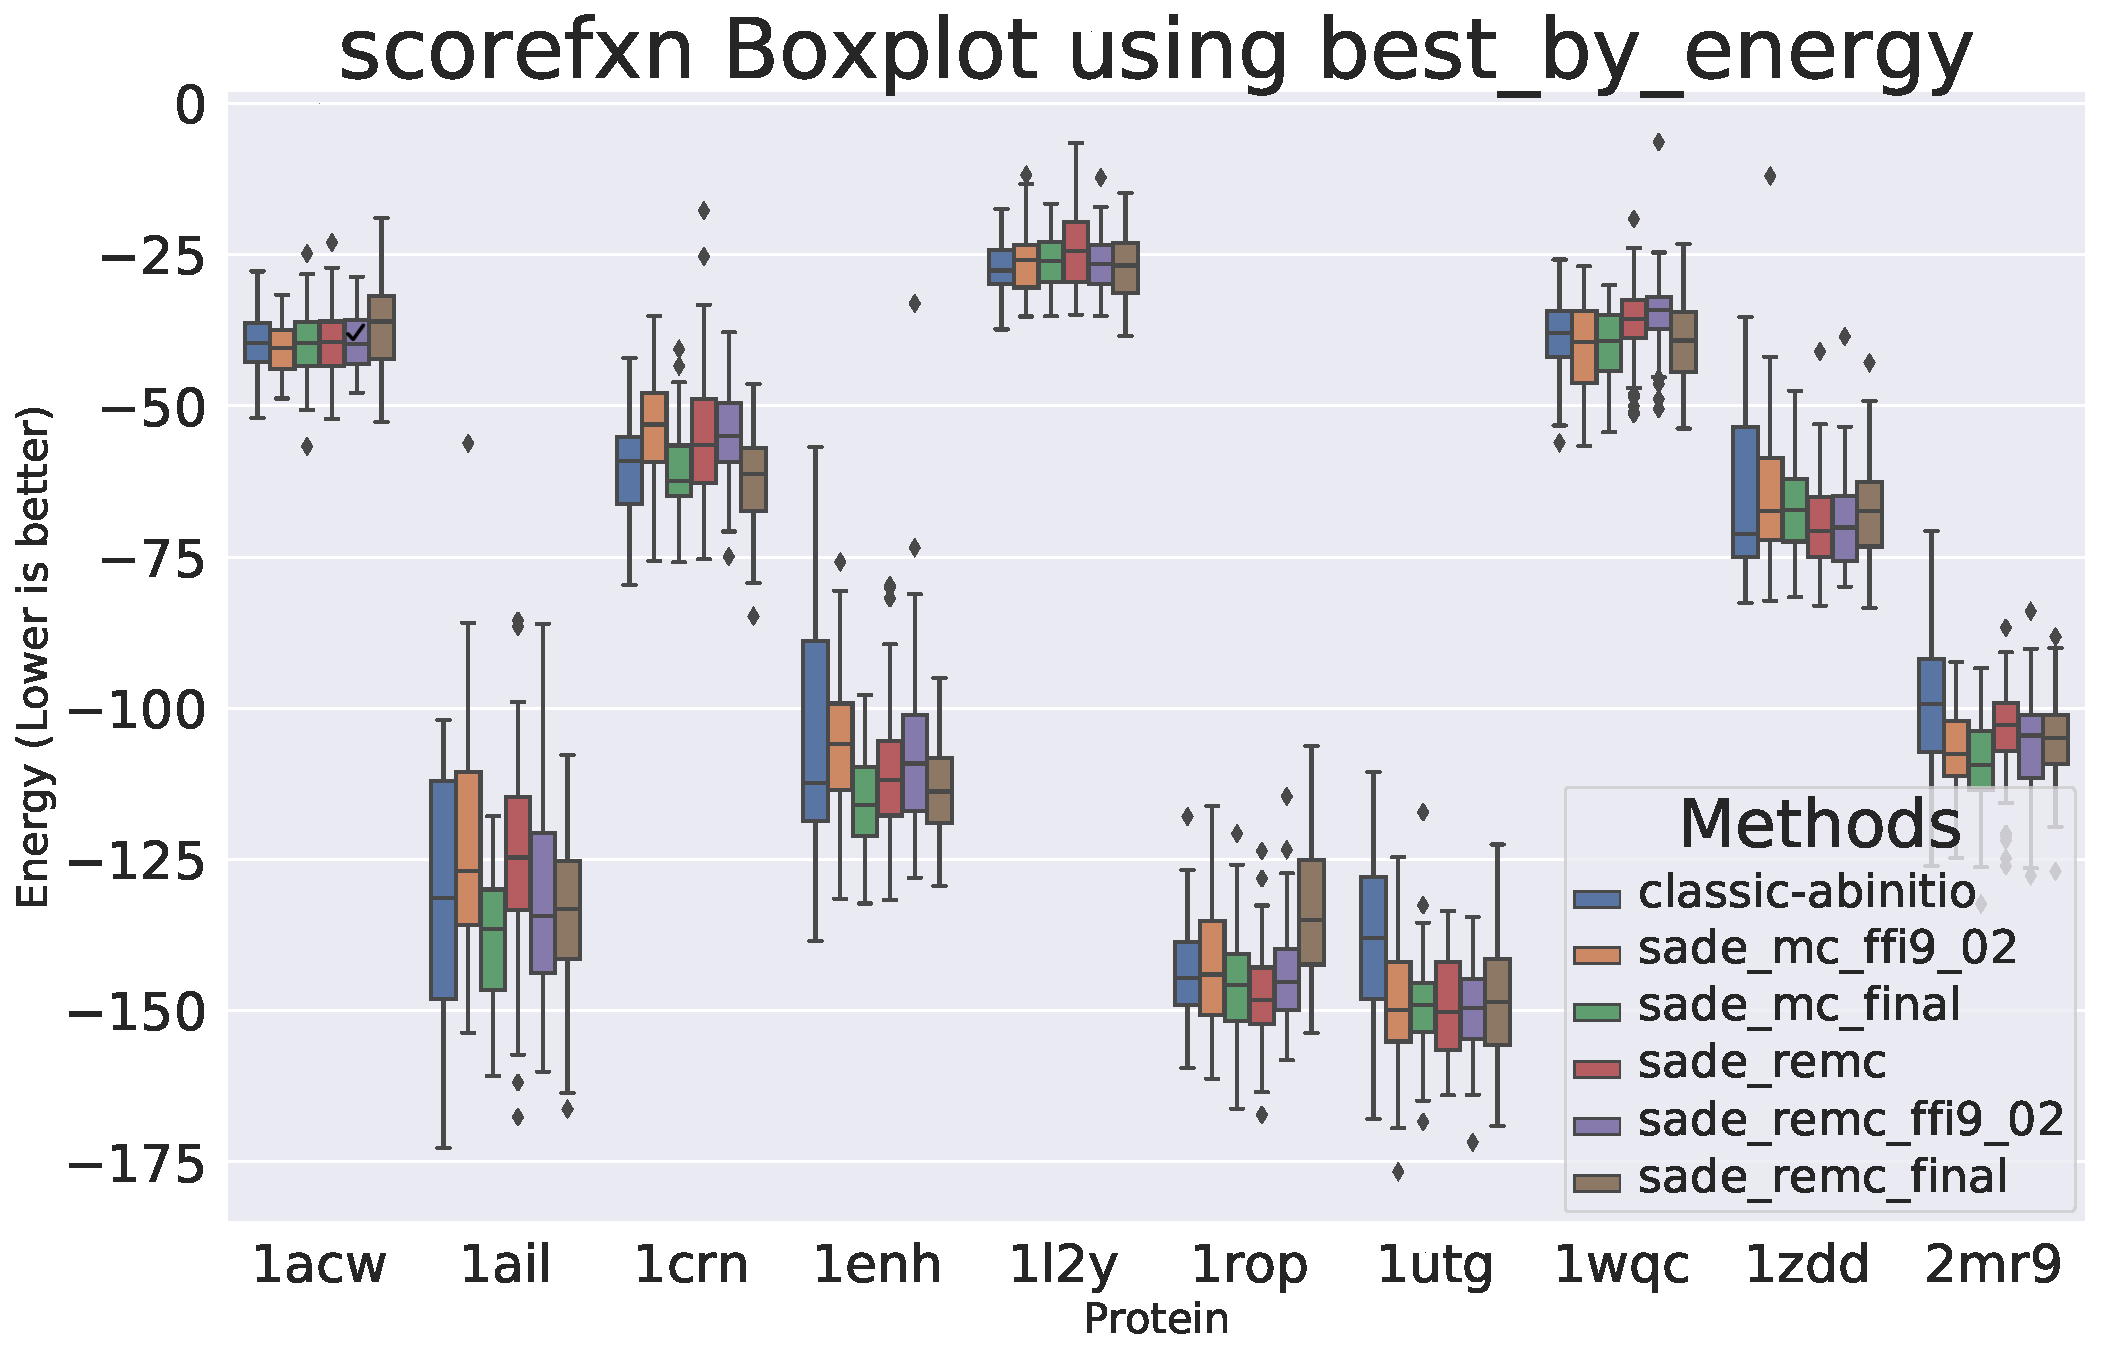
\includegraphics[width=\linewidth]{Figuras/boxplots/boxplot_best_by_energy_scorefxn.pdf}
  \caption{Boxplot presenting the \texttt{scorefxn} for the protein predictions with the
    competing methods. For the two proposed methods, the \texttt{best-by-energy}
    data was used}
  \label{fig:boxplot-energy}
\end{figure}

% \subsection{Statistical Analysis}
% \label{sec:statistical-analysis}

% Present Shapiro-Wilk RESULTS
To scientifically assess the performance of the proposed methods relative to
other competing methods, proper statistical tests are required. A prerequisite
before applying the tests which evaluate performance is to detect the
underlying distribution of the data to be analysed. There are several ways to
accomplish this. One, is to visually inspect a histogram or a Quantile-Quantile
plot. A more rigorous approach is to use a statistical test which can evaluate
the presence of a gaussian distribution. One such test is the Shapiro-Wilk and it
will be utilized for this purpose.

For the statistical analysis, an $\alpha = 0.05$ was utilized indicating a confidence level of 5\%. The RMSD and \texttt{scorefxn} of both the \texttt{best-by-rmsd} and \texttt{best-by-energy} were analysed for all the methods. For the sake of brevity the results are exposed outside this
text, in Appendix~\ref{appendix:shapiro}. The null hypothesis, $H_0$, is that
the samples belong to a normal distribution. Therefore, if the test returns a $p$
value less than $\alpha$, $H_0$ is rejected and the underlying distribution is
not gaussian. If $p$ is equal or bigger than $\alpha$, then the test failed to
reject $H_0$. Considering the data to be analyzed, this is not so straight
forward. There are 2 metrics to be analysed, the RMSD and \texttt{scorefxn}.
There are several methods which were executed. Furthermore, several proteins
were utilized for testing. Not only this gives a big amount of data to analyze,
it is possible that some method, protein or metric may lead to a gaussian
distribution, where others don't.

\textcolor{red}{
The tests were applied for RMSD and Energy, which lead to mixed results. Some
combinations of methods and proteins had gaussian distributions while others did
not. Considering this, both Kruskal-Wallis and Mann-Whitney tests can deal with
both gaussian and non-gaussian distributions with little cost of accuracy.
}
%
% For the RMSD using \texttt{best-by-rmsd}, there were $37$ cases where $H_0$
% failed to be rejected, and $23$ where it was rejected. All methods when applied
% to protein 1acw gave a gaussian distribution. For 1zdd, 5 of the 6 methods gave
% a non-gaussian distribution. The proteins, 1crn, 1l2y and 2mr9, had split results
% where half the methods rejected $H_0$ and half didn't. Some proteins appear to
% be more propense to generate gaussian distributions than others. By analysing
% the methods instead of the proteins, a new insight is given. The two proposed
% methods had $2$ and $1$ rejection of $H_0$, for ppf-mc and ppf-remc,
% respectively. Whereas sade-mc-ffi and SADE-REMC both had $6$ rejections. This
% indicates that some methods are more propense to generate gaussian distribution
% than others.
% 
% Considering \texttt{scorefxn} with \texttt{best-by-energy}, there were $46$
% cases where $H_0$ failed to be rejected, and $14$ were it was rejected. On this
% situation, with the given metric, more methods are generating gaussian
% distributions. Three proteins, 1acw, 1crn and 1l2y, failed all times to reject $H_0$.
% For 1ail and 1enh, the results were split in the middle. 1zdd had the most
% rejections of $H_0$, with $4$. The remaining proteins had only a single
% rejection of $H_0$. with both metrics, 1zdd had the most rejections of $H_0$,
% whereas all methods on 1acw failed to reject $H_0$. Looking at the methods,
% there is no clear trend. The proposed method ppf-remc had no rejection
% of $H_0$, while ppf-mc had two.
%
% Conclude the analysis and introduce the next analysis
% Given this, it appears that the underlying distribution, in most cases,
% is gaussian. However, there are consistent, albeit fewer, situations where they are
% not gaussian. As such, a non-parametric test must be employed.
%
In this case, the analysis is split in two steps.
Firstly, Kruskal–Wallis test is applied in order
to detect if there is a significant difference between the distribution, i.e.
if there is a method that is better than some other. If there is, then
a pairwise Mann-Whitney is utilized. Even though it is a non-parametric test, it
has, relative to Student's t test, a similar performance. Therefore,
Mann-Whitney's test can suit the needs to analyse the data at hand. Running
Mann-Whitney only if Kruskal–Wallis detects a significant difference is
important, as it helps to prevent inference errors.

% Present kruskal-wallis RESULTS
The Kruskal–Wallis test was performed with an $\alpha = 0.05$. The null-hypothesis
is that all the samples were drawn from the same distribution, i.e. all the
methods have equivalent performance.
Table~\ref{tab:kruskal-wallis-best-by-rmsd-RMSD} presents the result of the
tests for the RMSD.
The column protein indicates the name of the protein, and the column
$p$-value indicates the result of the test. When the $p$-value is less than
$\alpha$ it is highlighted in boldface. The result if very straightforward to
interpret. All the proteins with the exception of 1zdd had a $p$-value less
than the selected $\alpha$. Moreover, when $H_0$ was rejected, the $p$-value
was less than $1e-05$ in all cases. For 1zdd, $H_0$ failed to be rejected, the
most likely reason is that since this protein is (arguably) the easiest one,
all methods reached near-native conformations.

Table~\ref{tab:kruskal-wallis-best-by-energy-scorefxn} reads the same
as the previous one, however, the data it displays regards to \texttt{scorefxn}.
Protein 1zdd failed to reject $H_0$ again, as did 1l2y, another relatively
simple and short protein. For all the remaining proteins $H_0$ was rejected.
Therefore, it is safe to do a pair-wise test using Mann-Whitney's.

\begin{table}
  \begin{minipage}{.5\linewidth}
  \centering
  \begin{tabular}{r|c}
  Protein & $p$-value \\ \hline \hline
  1acw & $\bm{0.0000}$ \\ \hline
  1ail & $\bm{0.0000}$ \\ \hline
  1crn & $\bm{0.0000}$ \\ \hline
  1enh & $\bm{0.0000}$ \\ \hline
  1l2y & $\bm{0.0000}$ \\ \hline
  1rop & $\bm{0.0000}$ \\ \hline
  1utg & $\bm{0.0000}$ \\ \hline
  1wqc & $\bm{0.0000}$ \\ \hline
  1zdd &     $0.4145$  \\ \hline
  2mr9 & $\bm{0.0000}$ \\ \hline
  \end{tabular}
  \caption{Kruskal-Wallis for \texttt{best-by-rmsd} using RMSD}
  \label{tab:kruskal-wallis-best-by-rmsd-RMSD}
  \end{minipage}
% \end{table}
%
% \begin{table}
  \begin{minipage}{.5\linewidth}
  \centering
  \begin{tabular}{r|c}
  Protein & $p$-value \\ \hline \hline
  1acw & $\bm{0.0177}$ \\ \hline
  1ail & $\bm{0.0000}$ \\ \hline
  1crn & $\bm{0.0000}$ \\ \hline
  1enh & $\bm{0.0001}$ \\ \hline
  1l2y &     $0.2930$  \\ \hline
  1rop & $\bm{0.0000}$ \\ \hline
  1utg & $\bm{0.0000}$ \\ \hline
  1wqc & $\bm{0.0001}$ \\ \hline
  1zdd &     $0.1558$  \\ \hline
  2mr9 & $\bm{0.0000}$ \\ \hline
  \end{tabular}
  \caption{Kruskal-Wallis for \texttt{best-by-energy} using scorefxn}
  \label{tab:kruskal-wallis-best-by-energy-scorefxn}
  \end{minipage}
\end{table}

% Present mann-whitney RESULTS
The Mann-Whitney test was applied with $\alpha = 0.05$. The null hypothesis is
that the two distributions are equal, i.e. both methods have the same
performance. Rejection of $H_0$ indicates that one method is better than other.
Considering that both RMSD and \texttt{scorefxn} will be analyzed, each for
10 proteins, a total of $20$ tables are necessary to expose all the data. As
such, this information is exposed in Appendix~\ref{appendix:mann-whitney-rmsd}
and~\ref{appendix:mann-whitney-scorefxn}, where the first presents the data for
RMSD and the second for the energy, respectively. The results will be summarized reporting the
overall results from the test. To keep focus and simplicity, first, the two
proposed methods will be compared against the other method. Then, they will be
compared against rosetta. In both cases, the RMSD and \texttt{scorefxn} will be
considered for the analysis.

\begin{table}
  \begin{minipage}{.5\linewidth}
  \centering
  \begin{tabular}{r|r|r|r}
  Protein & Wins & Loses & Draws \\ \hline \hline
   1acw &  6 &  0 &  4 \\ \hline
   1ail &  6 &  0 &  4 \\ \hline
   1crn &  7 &  1 &  2 \\ \hline
   1enh &  4 &  0 &  6 \\ \hline
   1l2y &  6 &  0 &  4 \\ \hline
   1rop &  4 &  3 &  3 \\ \hline
   1utg &  6 &  0 &  4 \\ \hline
   1wqc &  6 &  0 &  4 \\ \hline
   1zdd &  0 &  0 & 10 \\ \hline \overtabline
   2mr9 &  3 &  0 &  7 \\ \hline
  \end{tabular}
  \caption{Summary of Mann-Whitney \texttt{best-by-rmsd} using RMSD compared agaisnt the previous methods}
  \label{tab:mann-whitney-summary-internal-best-by-rmsd-RMSD}
  \end{minipage}
%\end{table}
%
%\begin{table}
  \begin{minipage}{.5\linewidth}
  \centering
  \begin{tabular}{r|r|r|r}
  Protein & Wins & Loses & Draws \\ \hline \hline
   1acw &  1 &  4 &  5 \\ \hline
   1ail &  5 &  1 &  4 \\ \hline
   1crn &  6 &  0 &  4 \\ \hline
   1enh &  5 &  0 &  5 \\ \hline
   1l2y &  1 &  0 &  9 \\ \hline \overtabline
   1rop &  1 &  4 &  5 \\ \hline
   1utg &  0 &  0 & 10 \\ \hline
   1wqc &  4 &  0 &  6 \\ \hline
   1zdd &  0 &  3 &  7 \\ \hline \overtabline
   2mr9 &  3 &  2 &  5 \\ \hline
  \end{tabular}
  \caption{Summary of Mann-Whitney \texttt{best-by-energy} using scorefxn compared agaisnt the previous methods}
  \label{tab:mann-whitney-summary-internal-best-by-energy-scorefxn}
  \end{minipage}
\end{table}

Starting with the RMSD using \texttt{best-by-rmsd}, comparing the two proposed
methods against the ones from a previous work, SADE-REMC, the results are shown in
Table~\ref{tab:mann-whitney-summary-internal-best-by-rmsd-RMSD}. The column
Protein displays the protein name.
Columns \textbf{Wins}, \textbf{Loses} and \textbf{Draws} show the number of
times that any of the two proposed methods outperformed, were outperformed,
or had the same performance than SADE-REMC (not including rosetta).
Based on the results from Kruskal–Wallis, as show in
Tables~\ref{tab:kruskal-wallis-best-by-rmsd-RMSD} and
Tables~\ref{tab:kruskal-wallis-best-by-energy-scorefxn}, there is no
difference between the methods for protein 1zdd both when considering RMSD and
\texttt{scorefxn}. For 1l2y also there is no difference, however, only with
\texttt{scorefxn}. As such, these rows in the table should be ignored.
\textcolor{red}{
These proteins are marked with an strike-through line in the following tables.
}

For all but two proteins, namely 1zdd and 1rop, the two proposed methods outperformed SADE-REMC.
On 1zdd, the three methods had statistically equivalent performance. For
1rop, SADE-REMC was able to outperform ppf-remc. Going back to the boxplots,
this was expected. Interestingly, for 1rop, ppf-mc outperformed SADE-REMC, which means
that ppf-mc also outperformed ppf-remc.

The summary concerning the energy of the conformations is show in
Table~\ref{tab:mann-whitney-summary-internal-best-by-energy-scorefxn}. It
reads the same as the table before.
For proteins 1ail, 1crn, and 1wqc the proposed methods both outperformed
SADE-REMC. On 1acw, SADE-REMC outperformed ppf-remc and was statistically
equivalent to ppf-mc. For 1enh only ppf-mc outperformed SADE-REMC. For 1rop
SADE-REMC outperformed ppf-remc. The only situation so far where all the
methods had statistically equivalent performance, without counting the results
from Kruskal–Wallis, was on 1utg and 1zdd.
Interestingly, on 1l2y, Mann-Whitney detected performance differences, disagreeing with
the results from Kruskal–Wallis. Nevertheless, for these protein, the result
from Kruskal–Wallis will be considered to be the correct one.

\begin{table}
  \begin{minipage}{.5\linewidth}
  \centering
  \begin{tabular}{r|r|r|r}
  Protein & Wins & Loses & Draws \\ \hline \hline
  1acw &  2 &  0 &  0 \\ \hline
  1ail &  1 &  0 &  1 \\ \hline
  1crn &  0 &  1 &  1 \\ \hline
  1enh &  2 &  0 &  0 \\ \hline
  1l2y &  2 &  0 &  0 \\ \hline
  1rop &  1 &  1 &  0 \\ \hline
  1utg &  2 &  0 &  0 \\ \hline
  1wqc &  0 &  0 &  2 \\ \hline
  1zdd &  0 &  0 &  2 \\ \hline \overtabline
  2mr9 &  2 &  0 &  0 \\ \hline
  \end{tabular}
  \caption{Summary of Mann-Whitney \texttt{best-by-rmsd} using RMSD compared agaisnt rosetta}
  \label{tab:mann-whitney-summary-rosetta-best-by-rmsd-RMSD}
  \end{minipage}
%\end{table}
%
%\begin{table}
  \begin{minipage}{.5\linewidth}
  \centering
  \begin{tabular}{r|r|r|r}
  Protein & Wins & Loses & Draws \\ \hline \hline
  1acw &  0 &  1 &  1 \\ \hline
  1ail &  1 &  0 &  1 \\ \hline
  1crn &  0 &  0 &  2 \\ \hline
  1enh &  1 &  0 &  1 \\ \hline
  1l2y &  0 &  0 &  2 \\ \hline \overtabline
  1rop &  0 &  1 &  1 \\ \hline
  1utg &  2 &  0 &  0 \\ \hline
  1wqc &  0 &  0 &  2 \\ \hline
  1zdd &  0 &  0 &  2 \\ \hline \overtabline
  2mr9 &  2 &  0 &  0 \\ \hline
  \end{tabular}
  \caption{Summary of Mann-Whitney \texttt{best-by-energy} using scorefxn compared agaisnt rosetta}
  \label{tab:mann-whitney-summary-rosetta-best-by-energy-scorefxn}
  \end{minipage}
\end{table}

In Table~\ref{tab:mann-whitney-summary-rosetta-best-by-rmsd-RMSD} the
two proposed methods is compared against Rosetta using RMSD. For 1acw, 1enh, 1l2y, 1utg and 2mr9, totalling 5 proteins, both
proposed methods outperformed rosetta. For 1ail only ppf-remc
outperformed rosetta. On 1rop, ppf-mc outperformed rosetta, while
ppf-remc was outperformed. On 1crn, only ppf-mc was outperformed
by rosetta. From this, it is demonstrated that both the proposed methods
consistently outperform rosetta. In fact, rosetta outperformed the proposed
methods only in 2 occasions when considering the RMSD.

The comparison of rosetta and the proposed methods using \texttt{scorefxn}
is presented in Table~\ref{tab:mann-whitney-summary-rosetta-best-by-rmsd-RMSD}.
For this particular case, for 2 proteins, 1utg and 2mr9, both proposed
methods outperformed rosetta. On 1acw and 1rop rosetta outperformed only
ppf-remc. On 1ail, only ppf-mc outperformed rosetta. Overall,
the proposed methods outperformed rosetta in some cases and had equal
significance in others.

In light of these observations, it is safe to consider that the two proposed
methods outperform the SADE-REMC. It also outperforms rosetta, one of
the state of the art methods in the literature and CASP winners.

\subsection{Pareto Front Analysis}\label{sec:pareto-front-analysis}

In this Section an analysis of the Pareto front of the four methods under
analysis is presented.
\textcolor{red}{
Considering that the end user would most likely only be
interested in the best prediction, this analysis considers the conformation with
the best RMSD and its respective energy, taken from all the runs of all methods under
analysis.
}

\begin{figure}
  \begin{subfigure}{0.49\linewidth}
    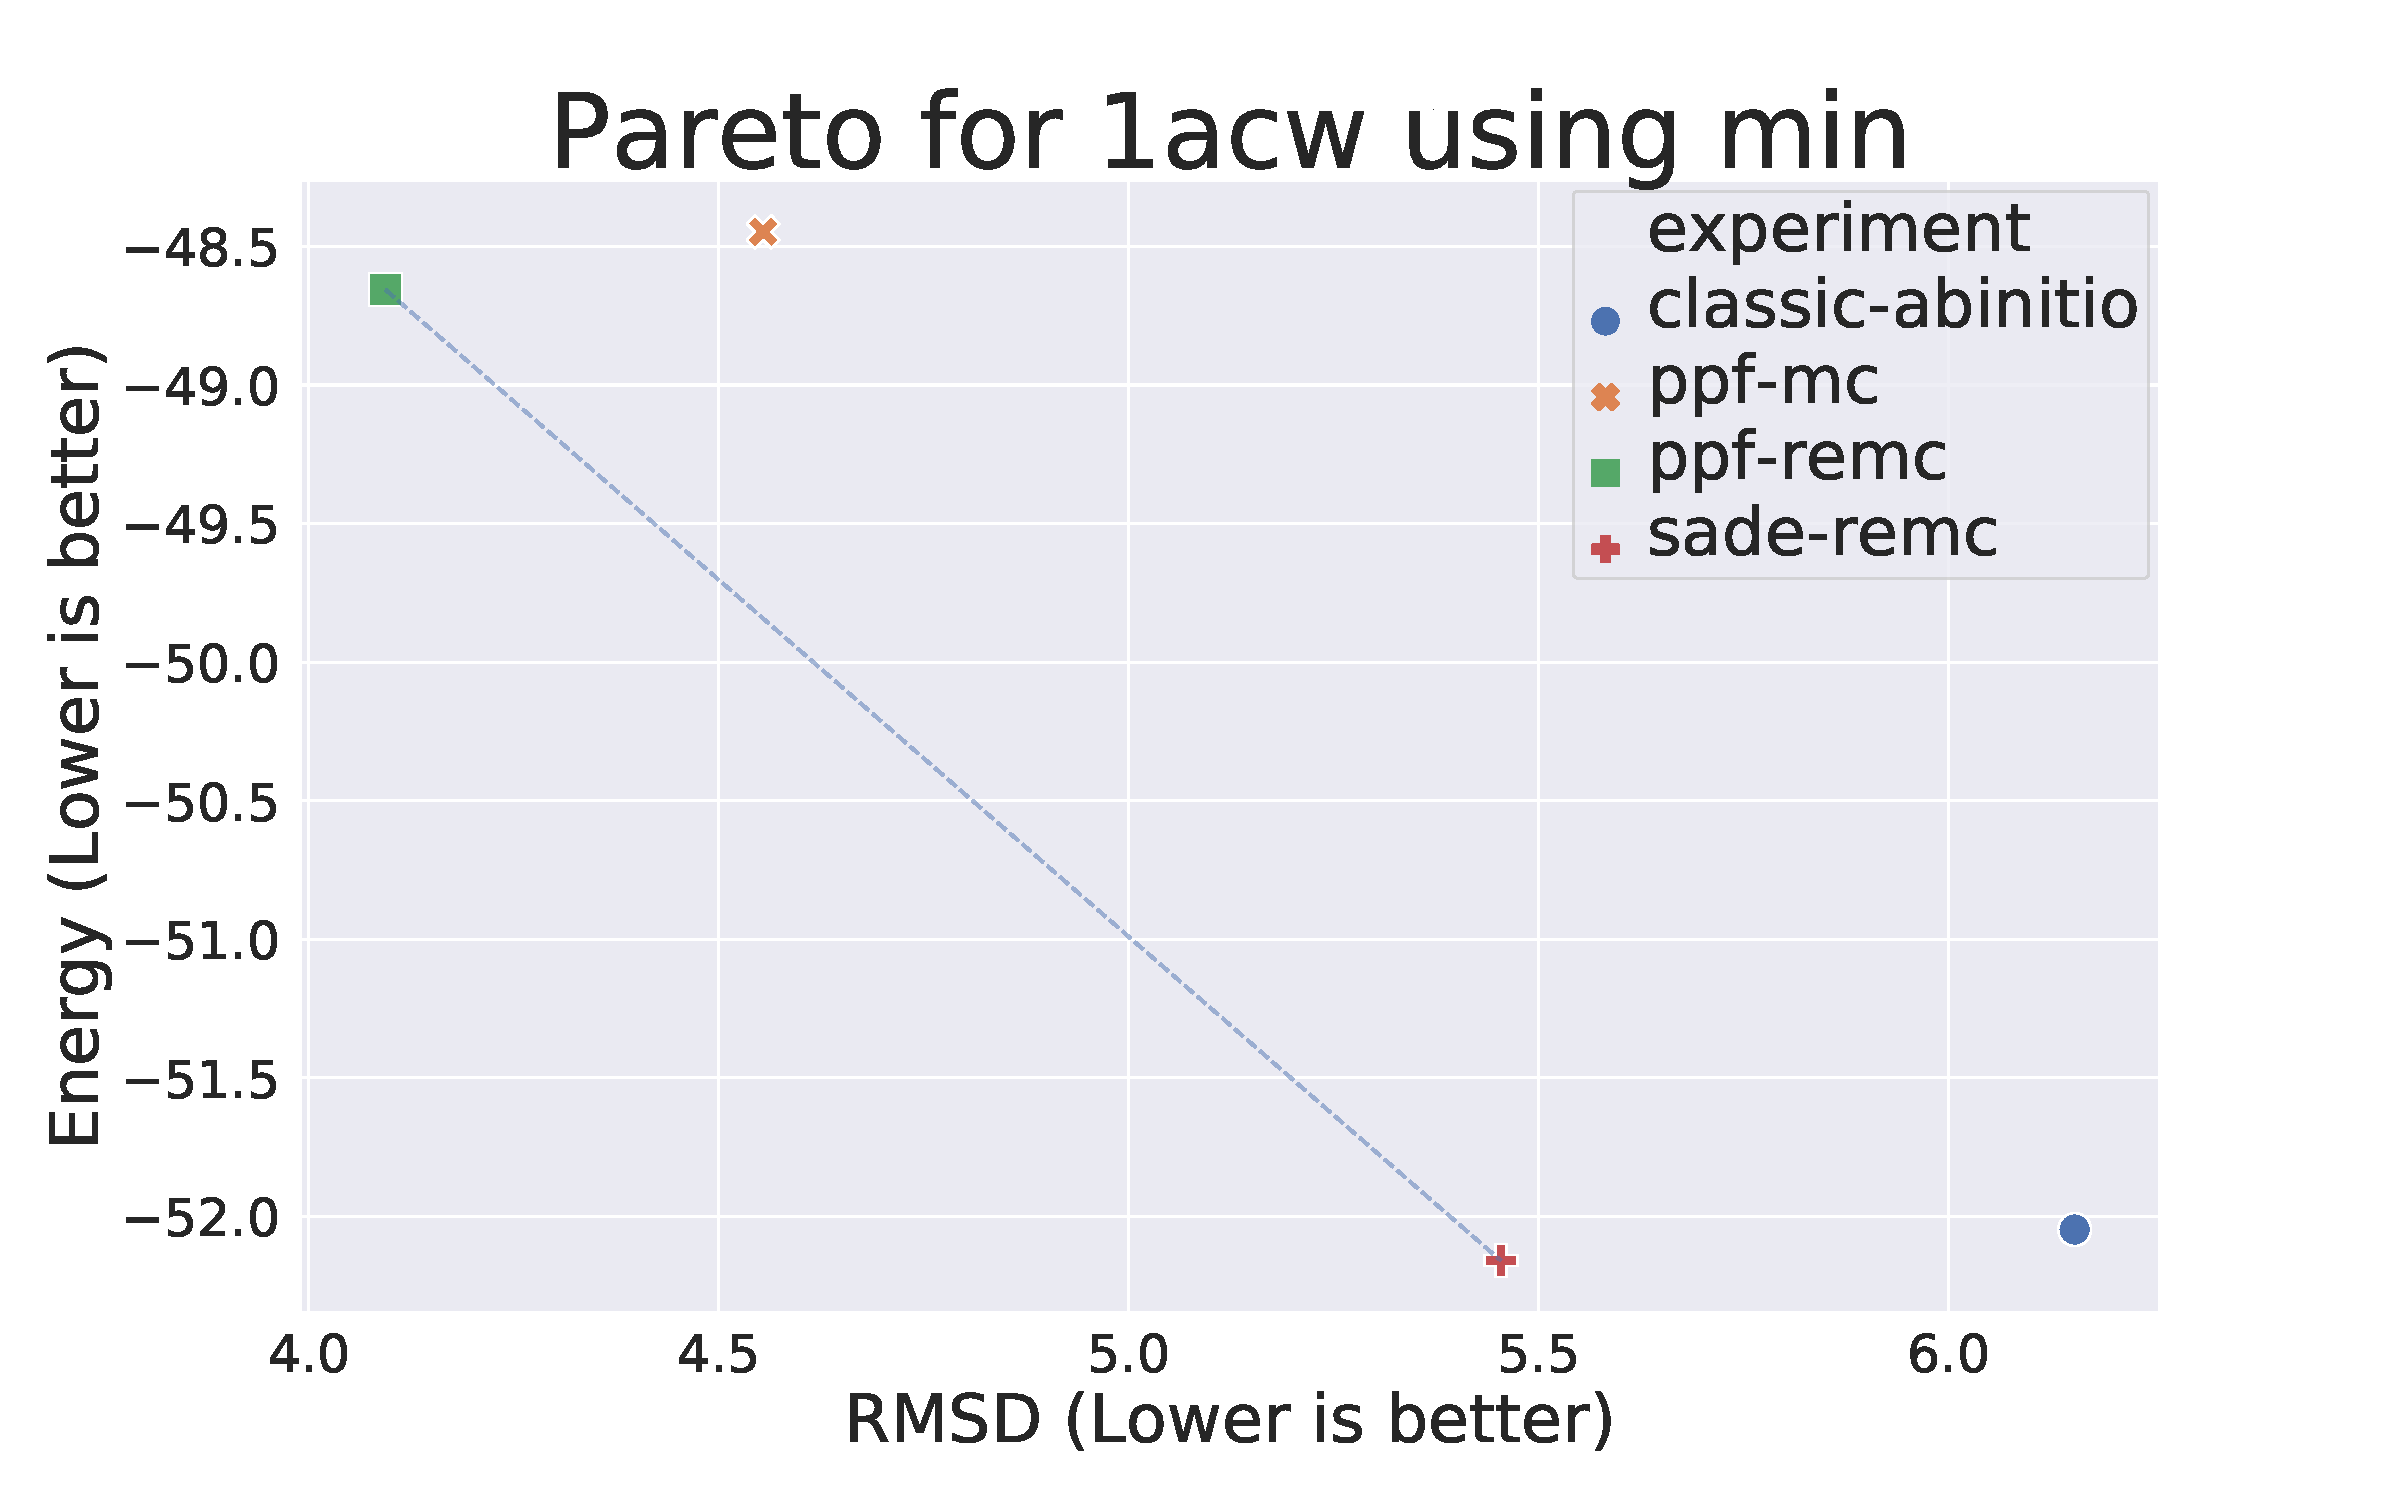
\includegraphics[width=1\linewidth]{Figuras/pareto/1acw_best_by_rmsd_min.pdf}
  \end{subfigure}
%
  \begin{subfigure}{0.49\linewidth}
    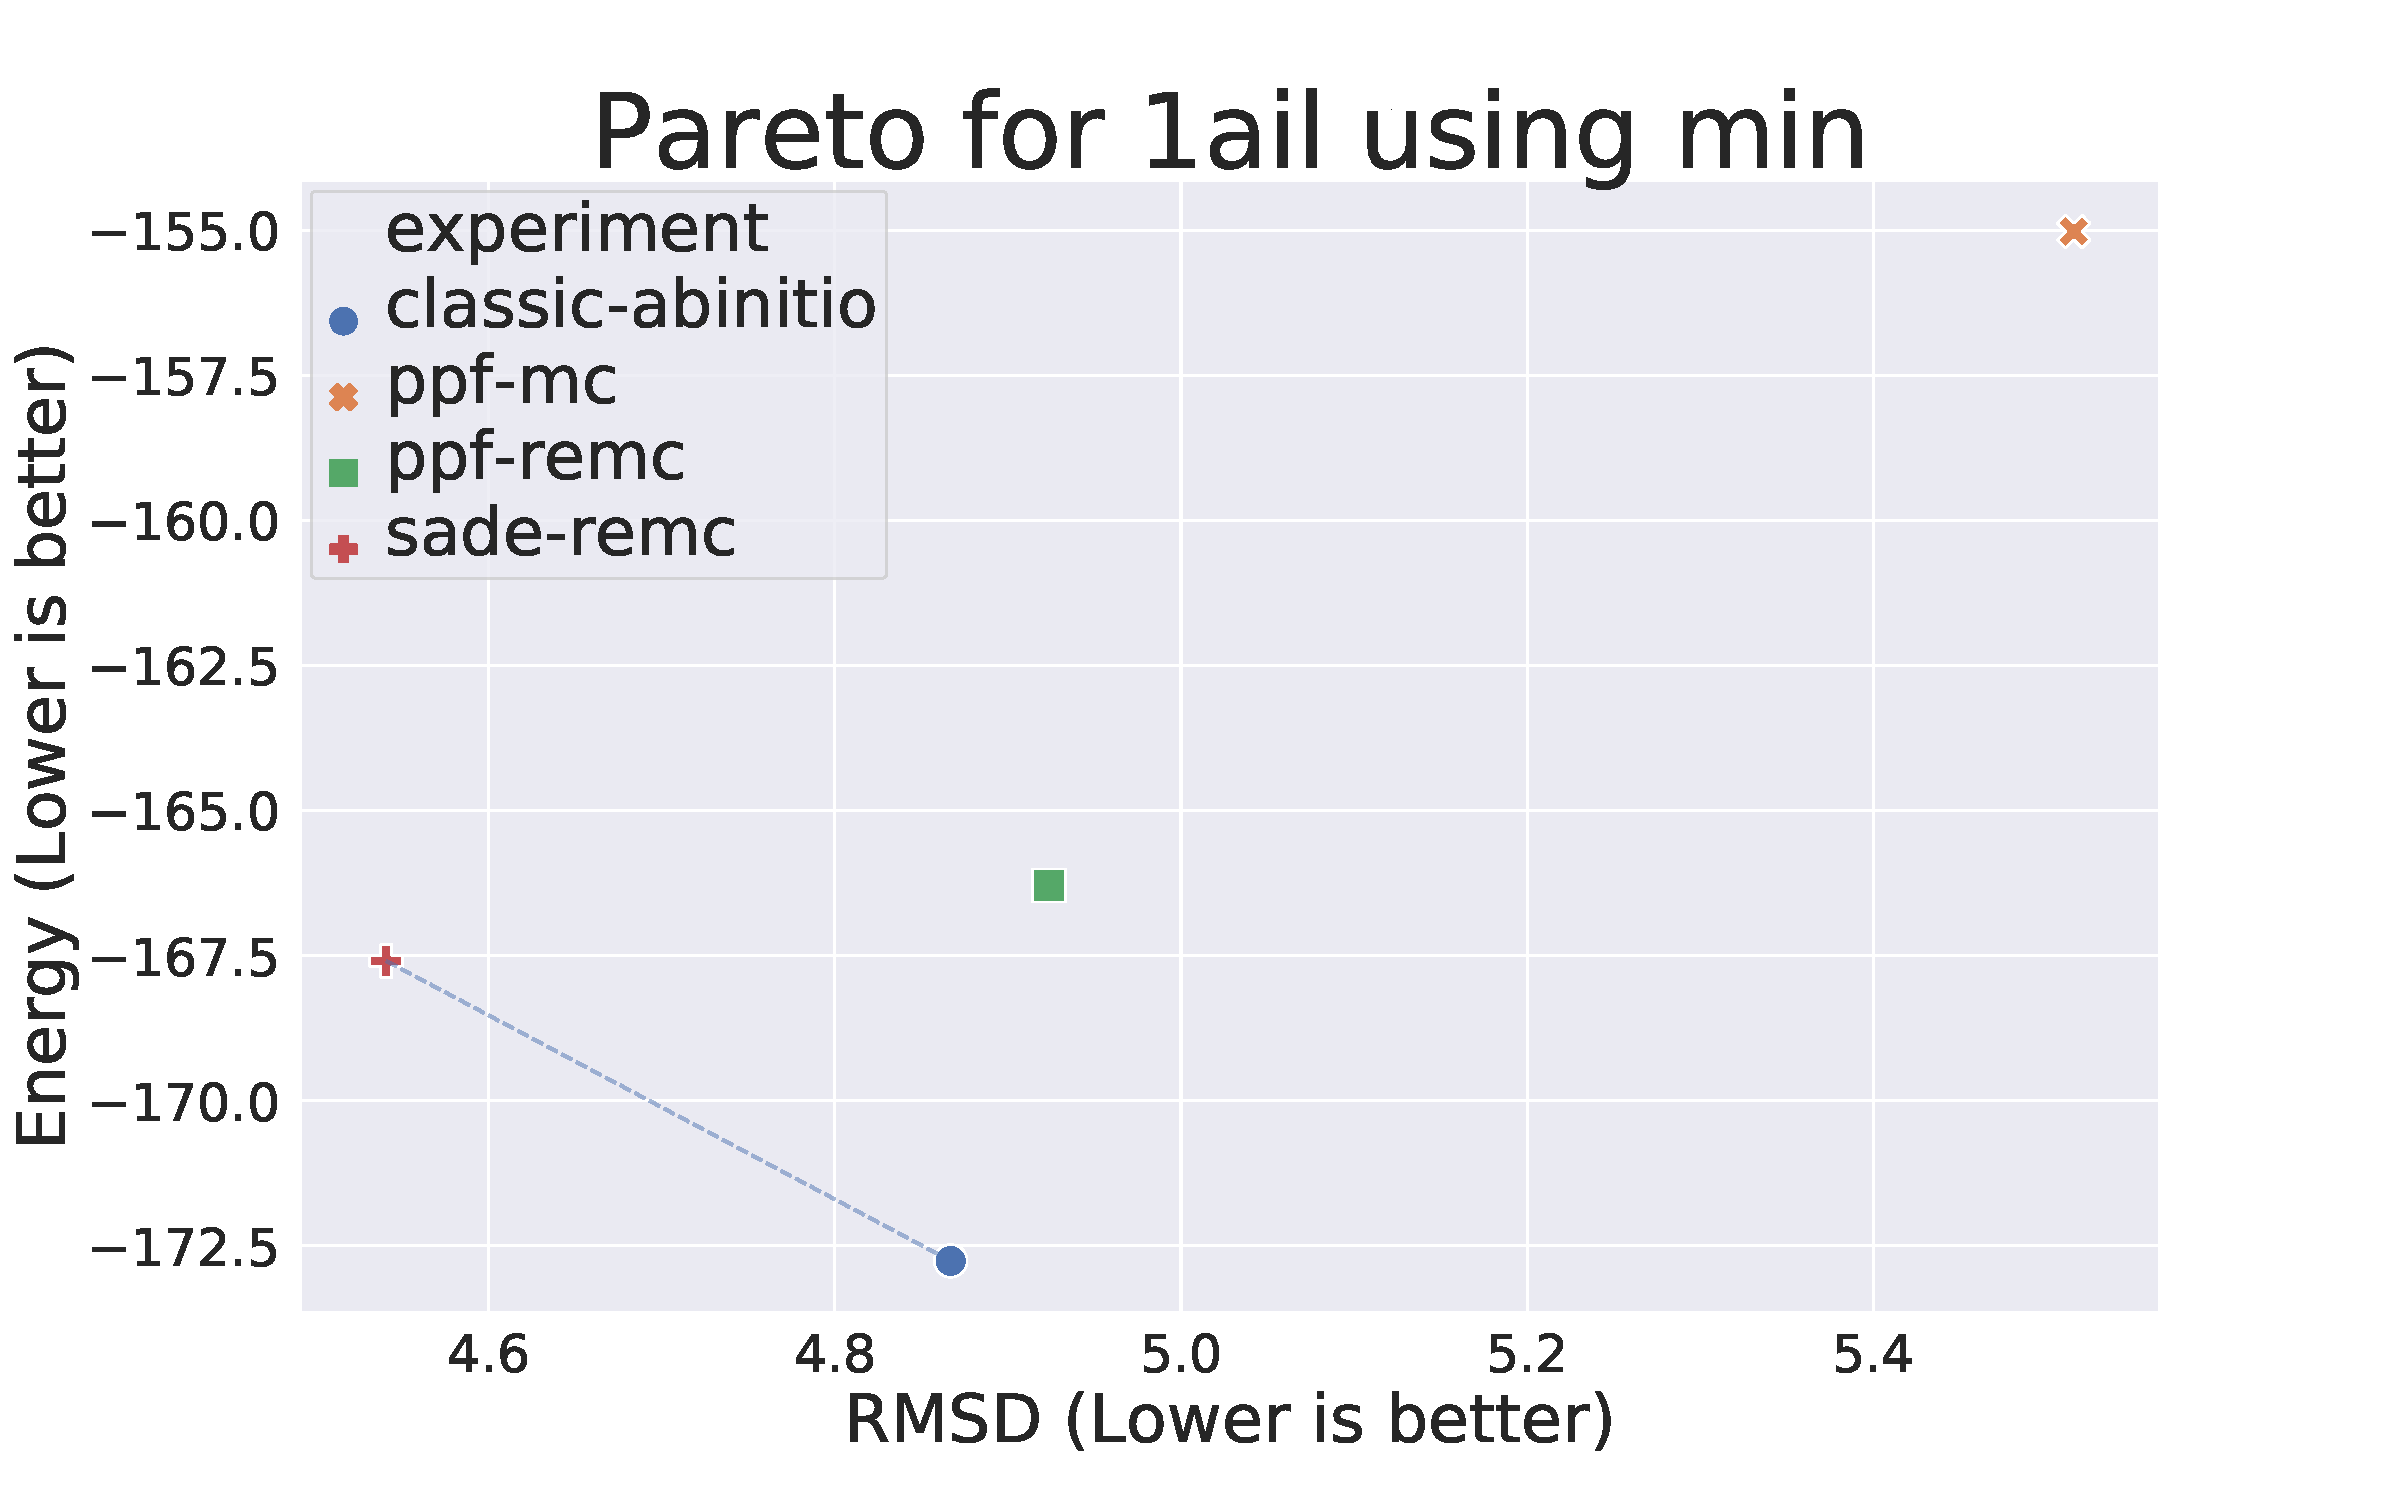
\includegraphics[width=1\linewidth]{Figuras/pareto/1ail_best_by_rmsd_min.pdf}
  \end{subfigure}
%
  \begin{subfigure}{0.49\linewidth}
    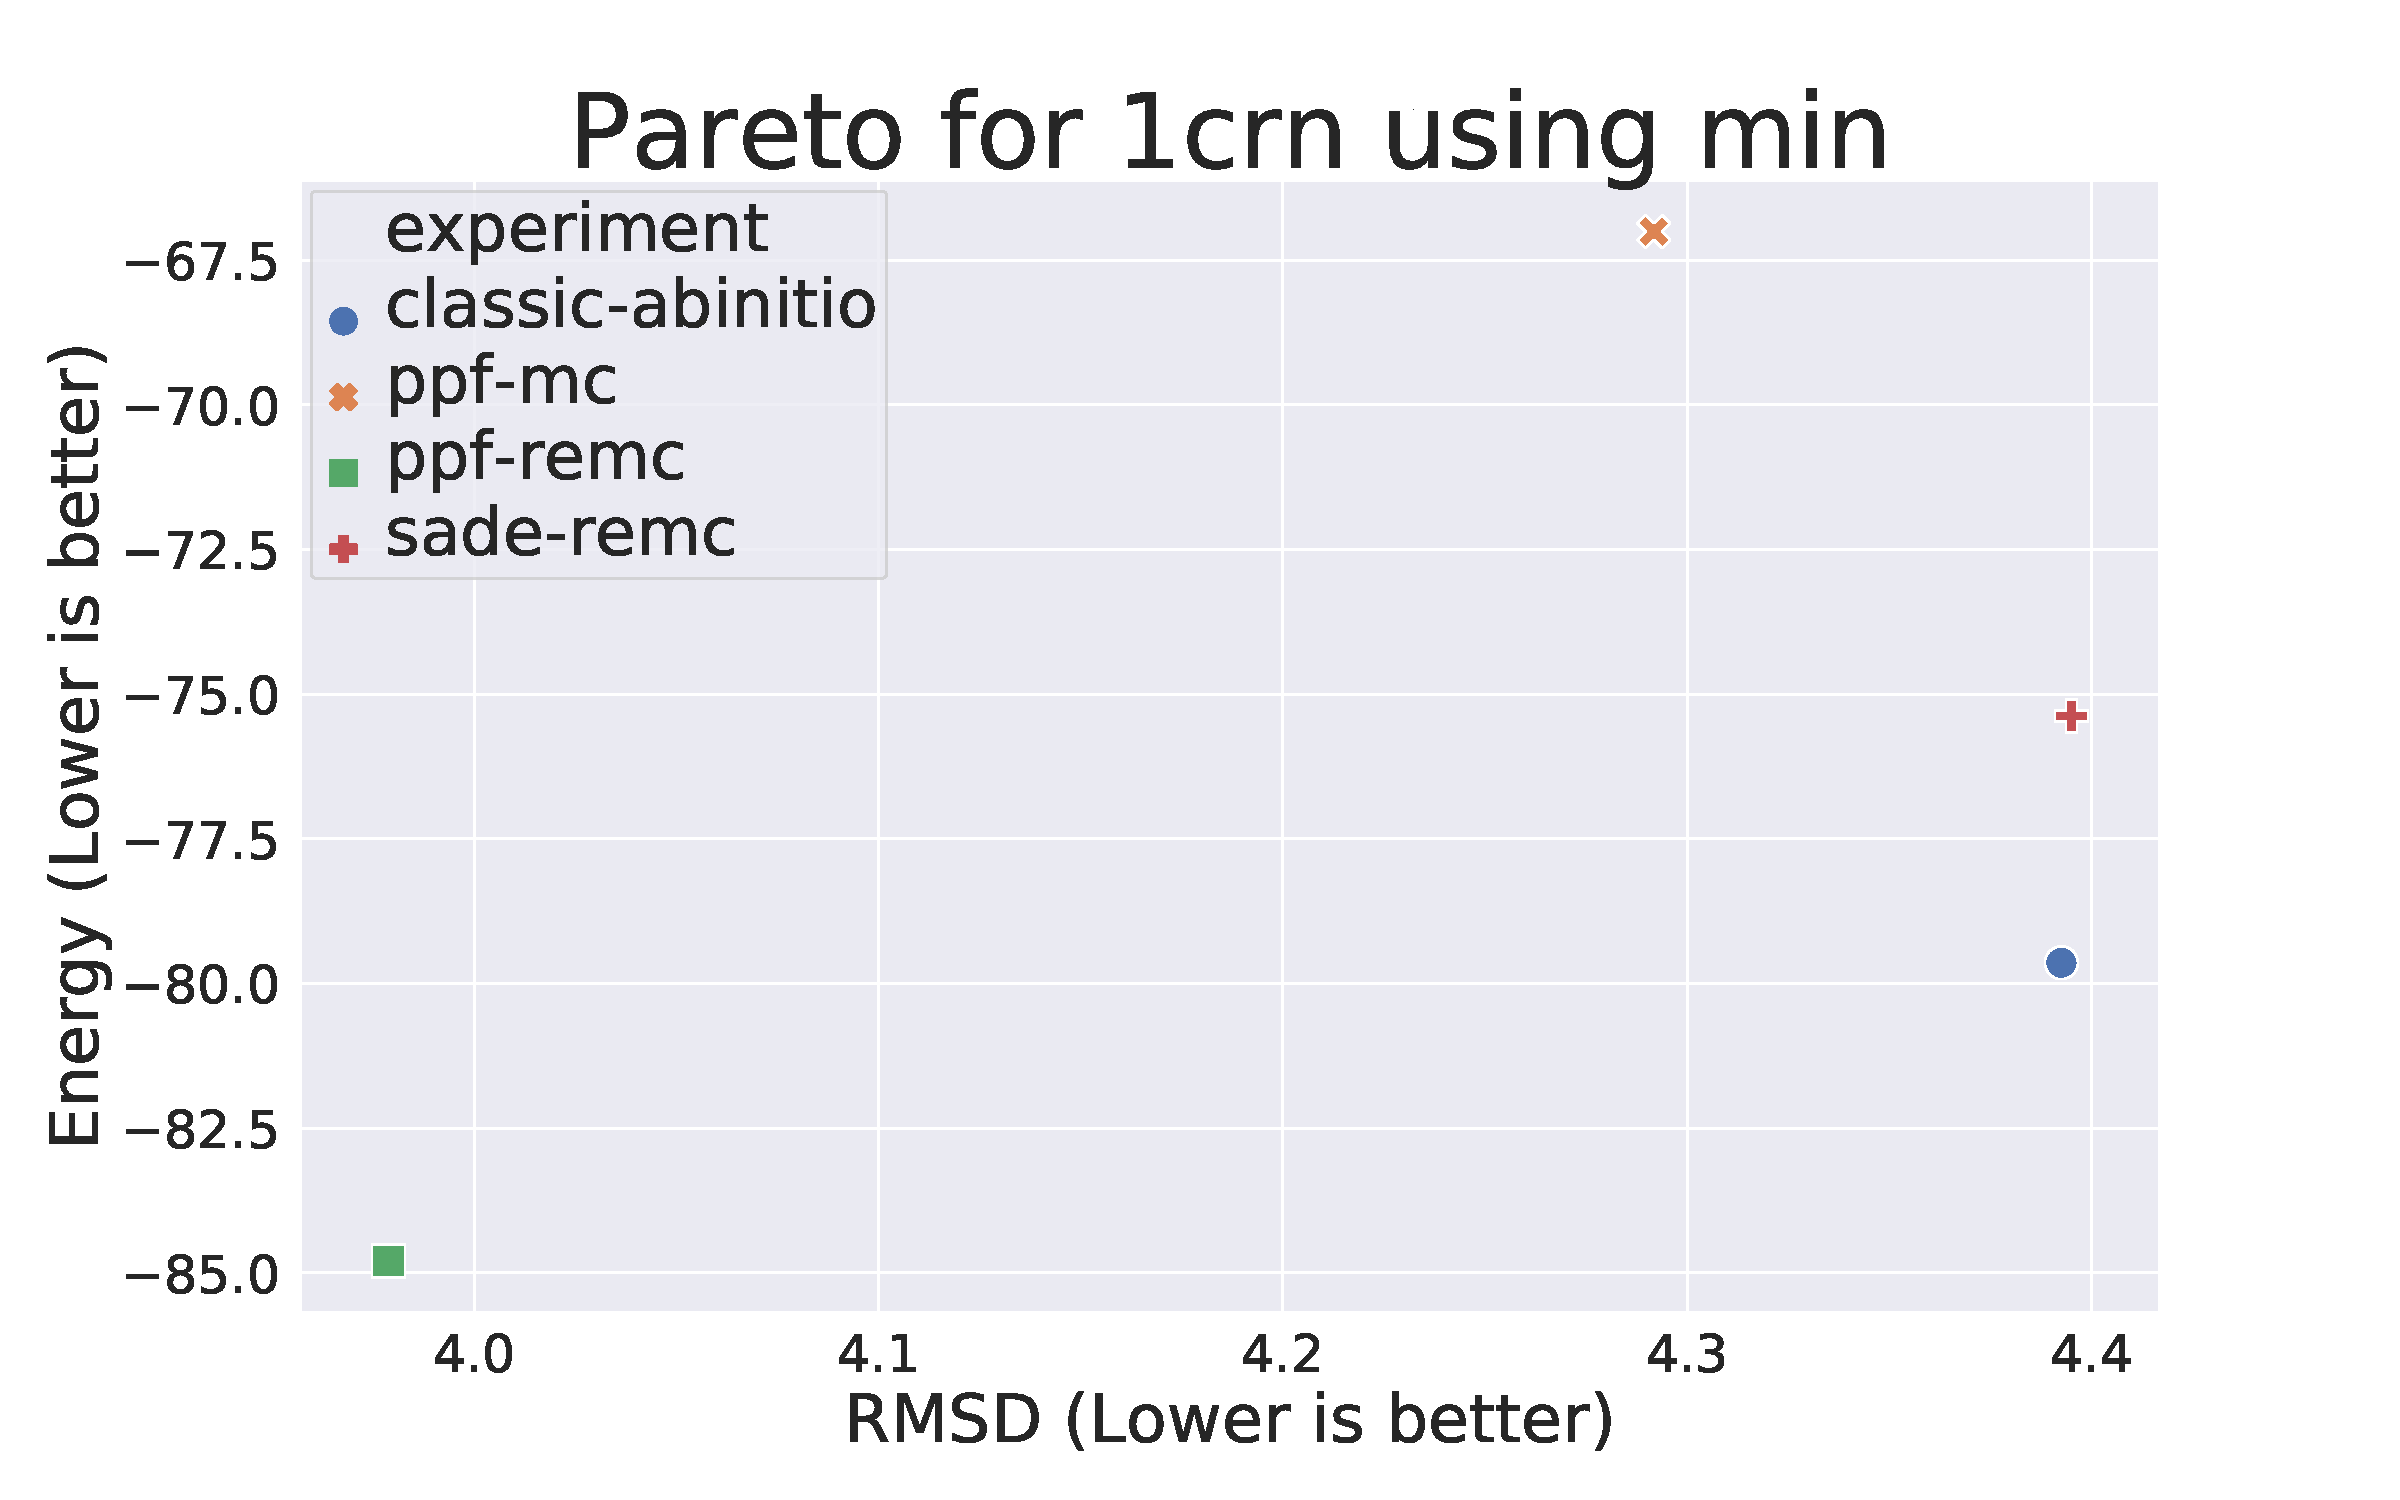
\includegraphics[width=1\linewidth]{Figuras/pareto/1crn_best_by_rmsd_min.pdf}
  \end{subfigure}
%
  \begin{subfigure}{0.49\linewidth}
    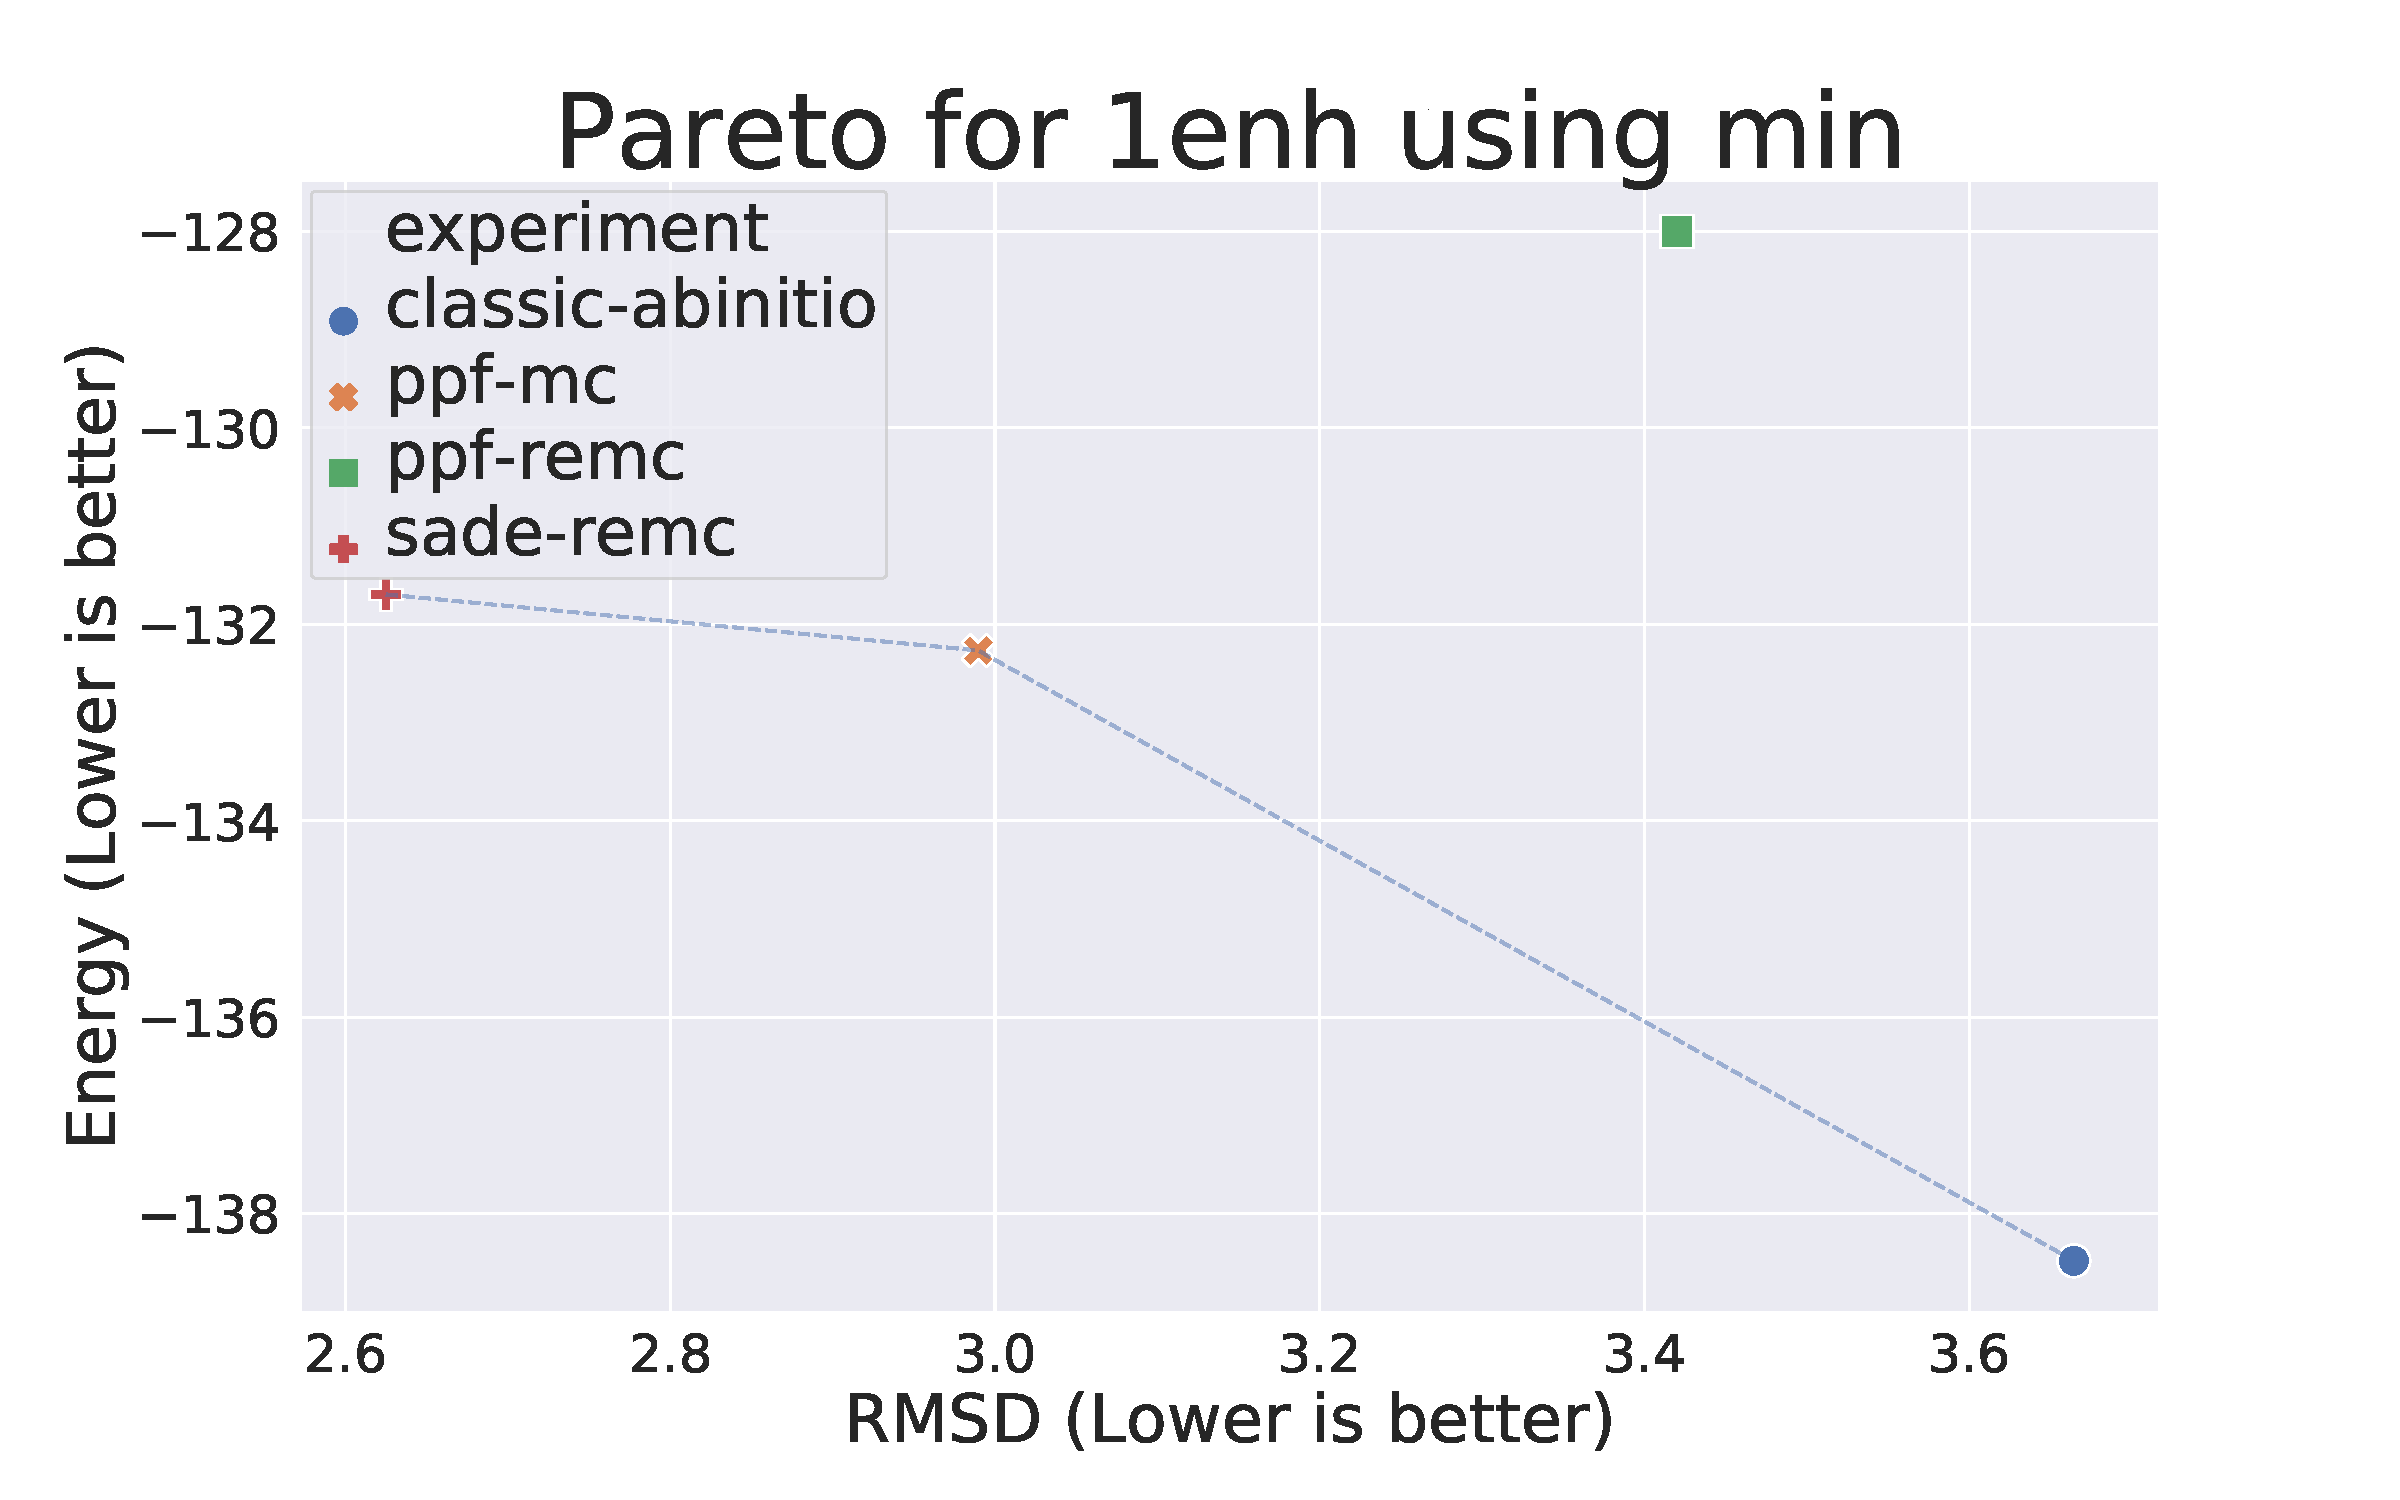
\includegraphics[width=1\linewidth]{Figuras/pareto/1enh_best_by_rmsd_min.pdf}
  \end{subfigure}
%
  \begin{subfigure}{0.49\linewidth}
    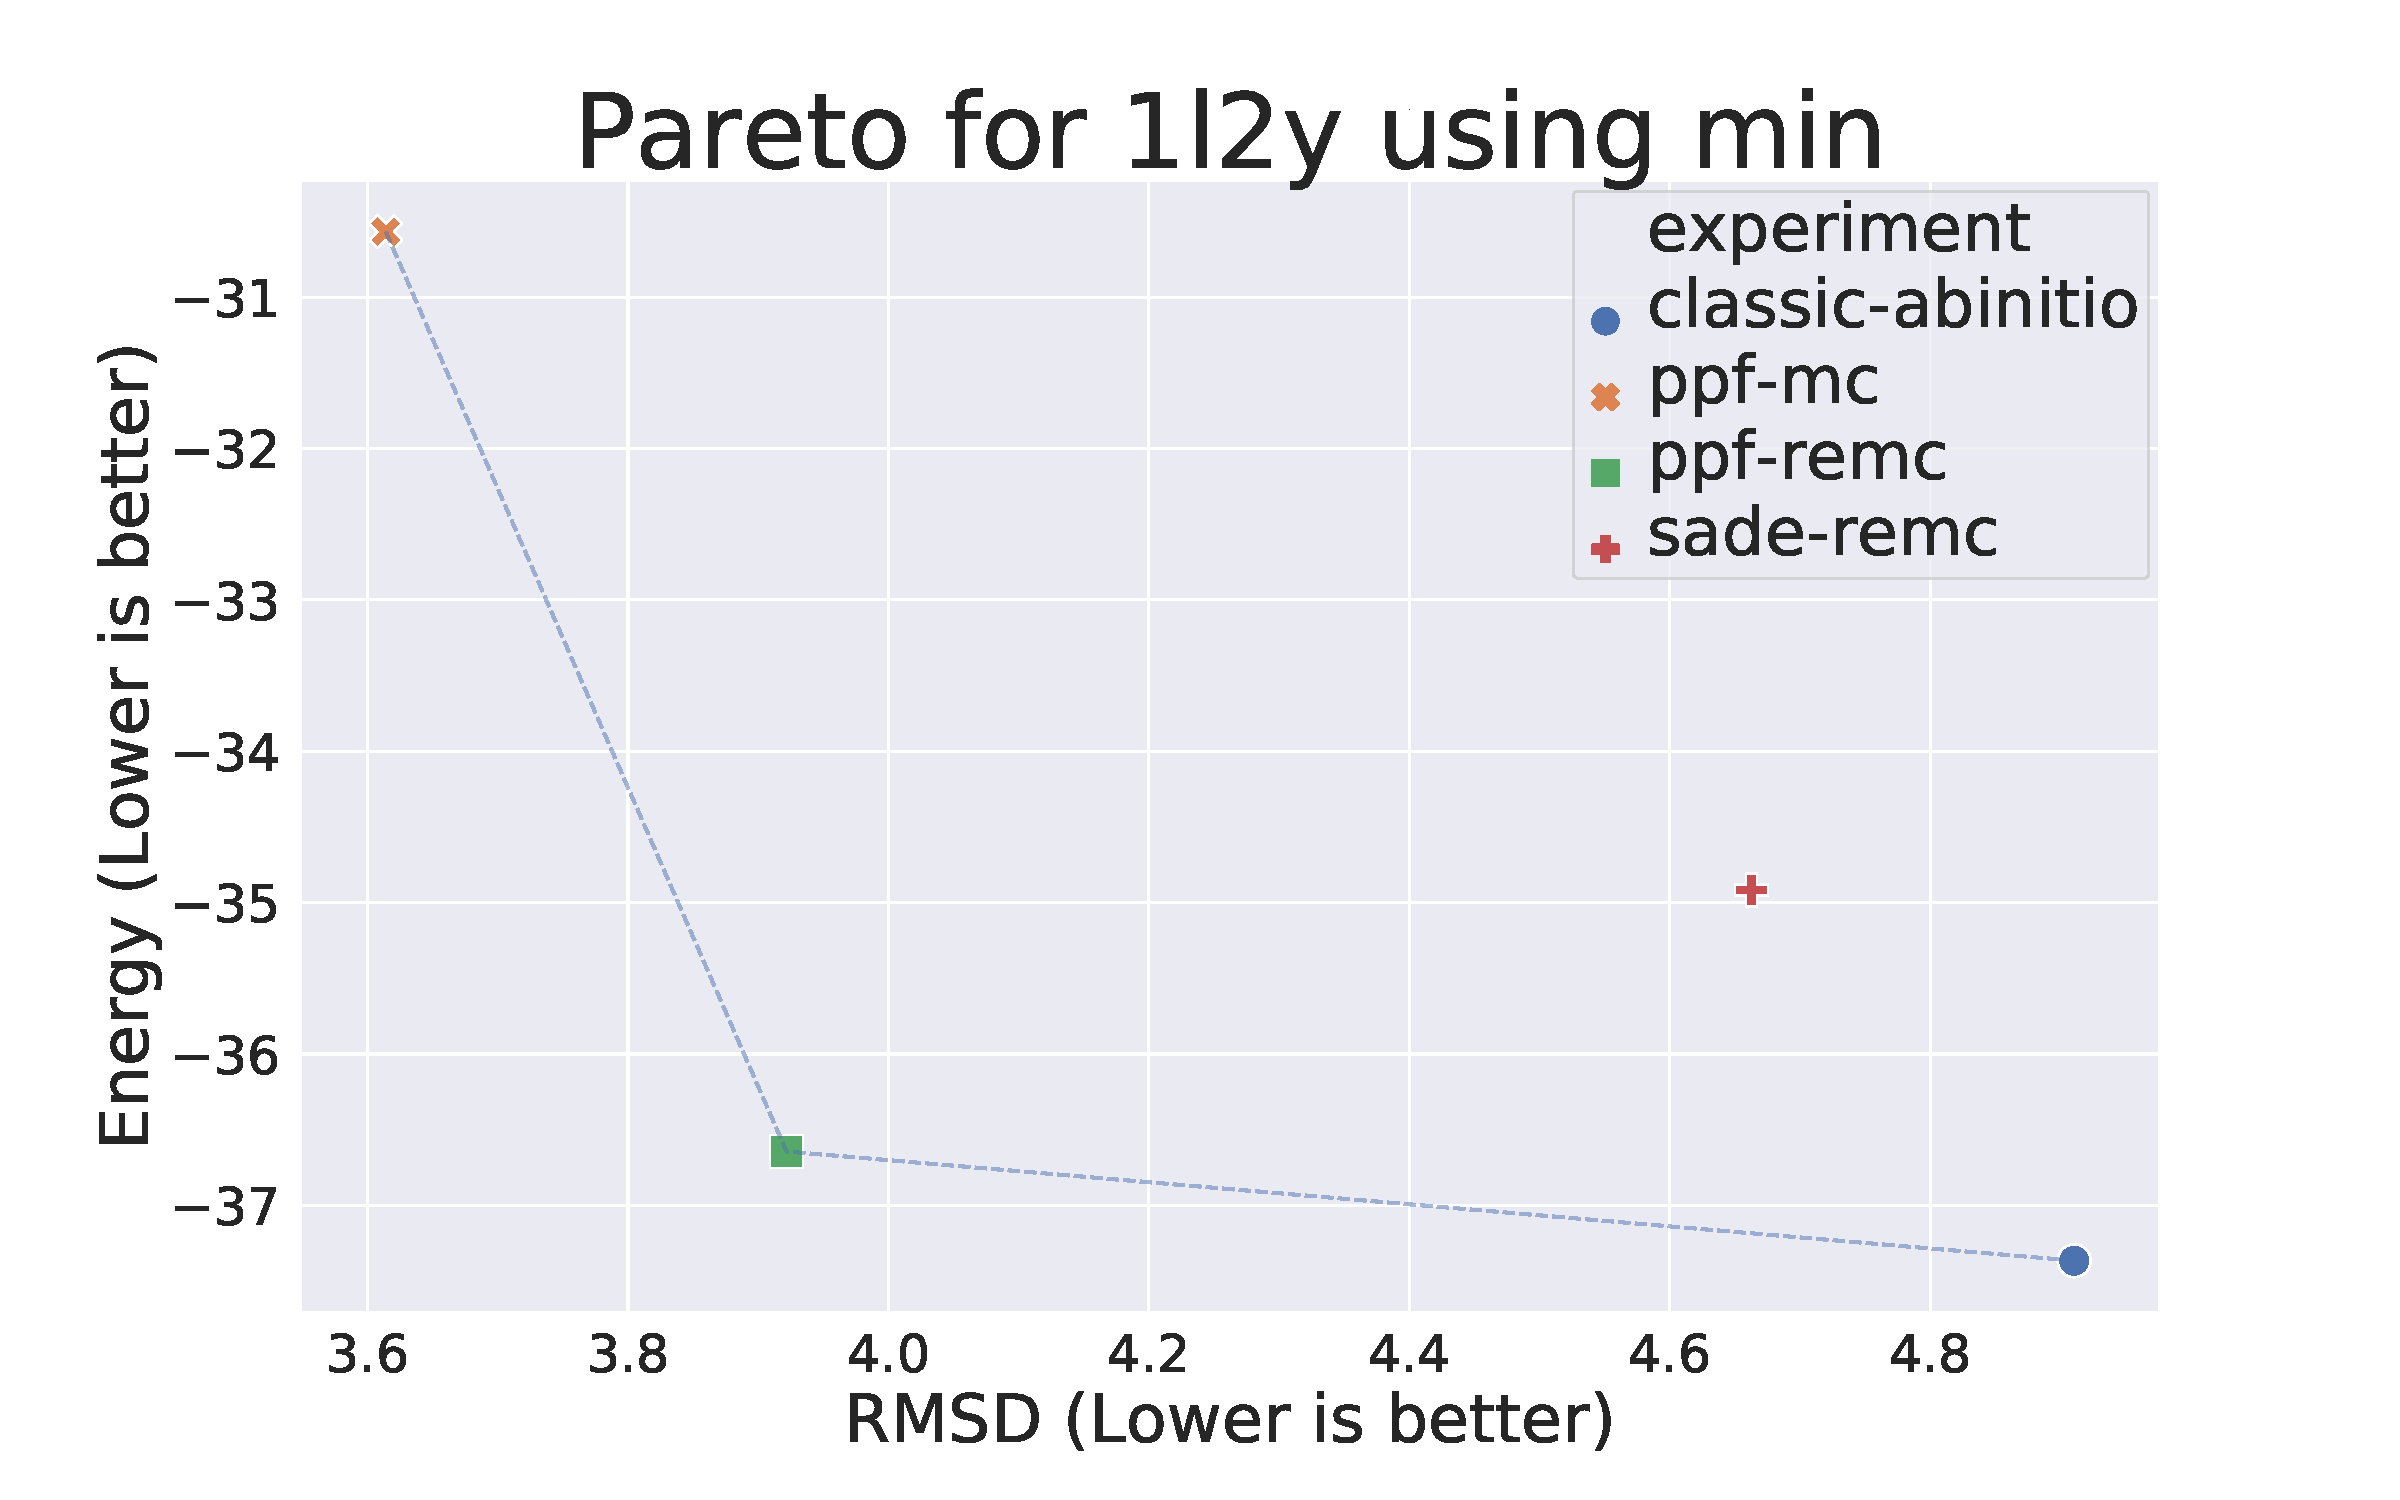
\includegraphics[width=1\linewidth]{Figuras/pareto/1l2y_best_by_rmsd_min.pdf}
  \end{subfigure}
%
  \begin{subfigure}{0.49\linewidth}
    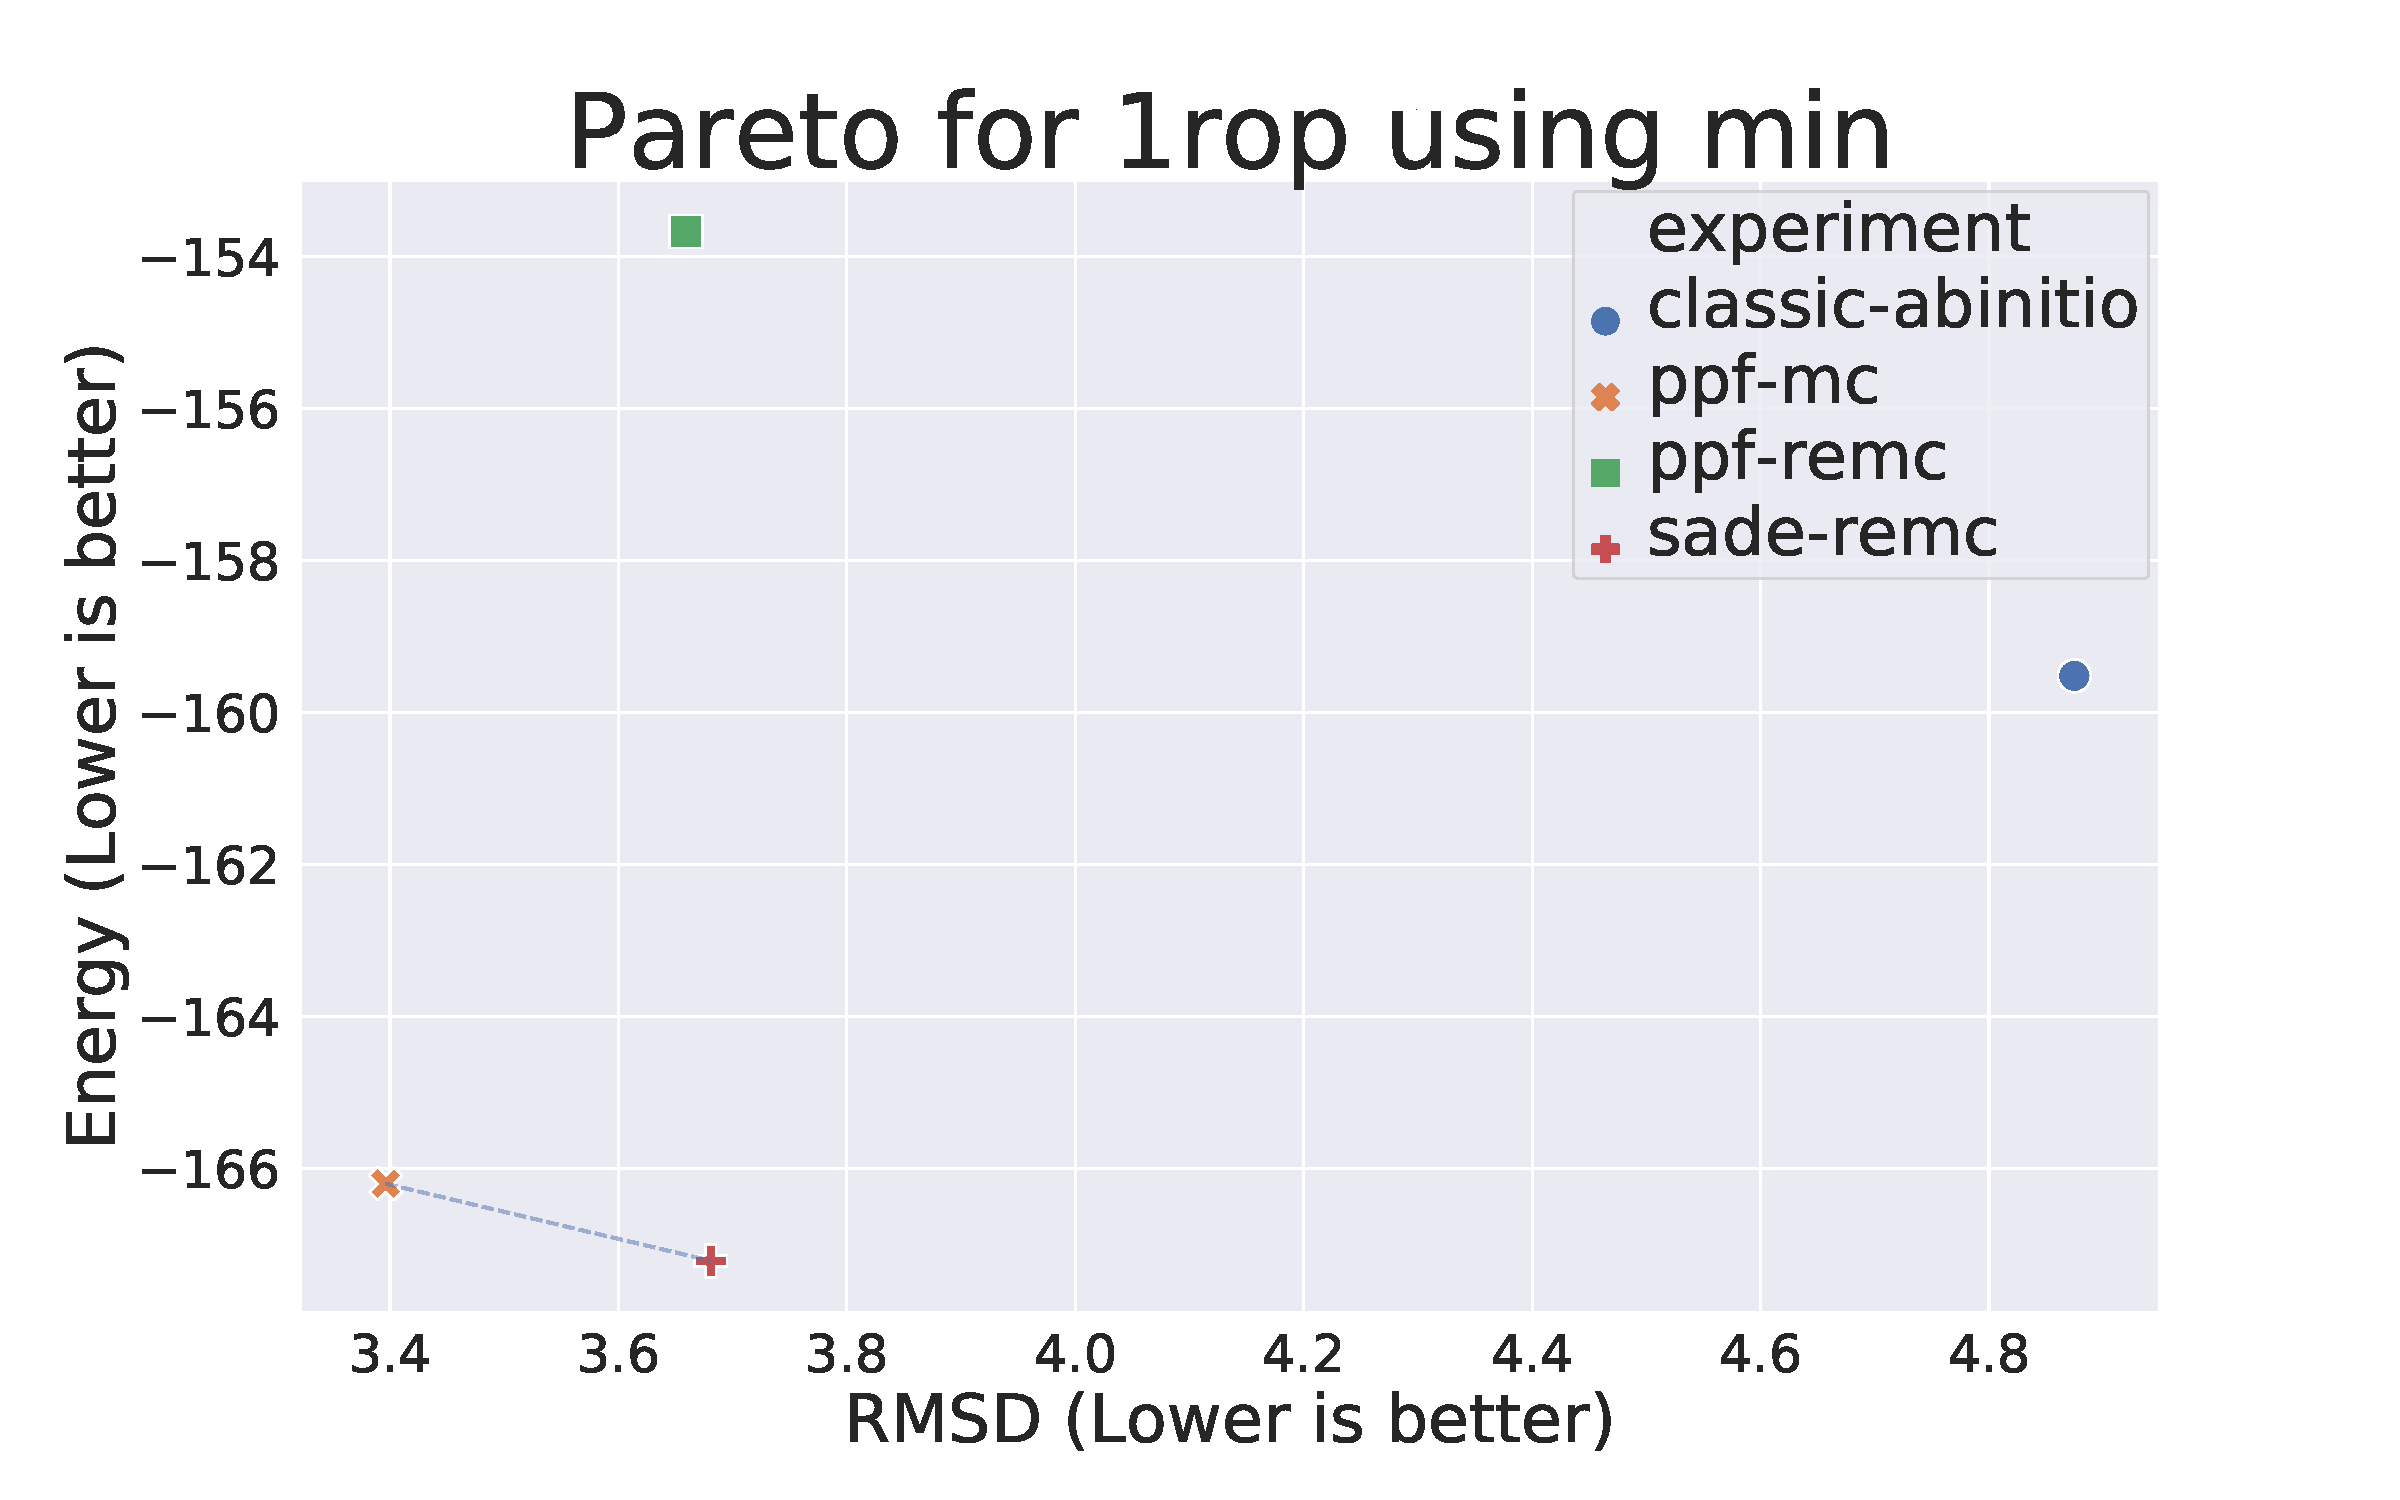
\includegraphics[width=1\linewidth]{Figuras/pareto/1rop_best_by_rmsd_min.pdf}
  \end{subfigure}
%
  \begin{subfigure}{0.49\linewidth}
    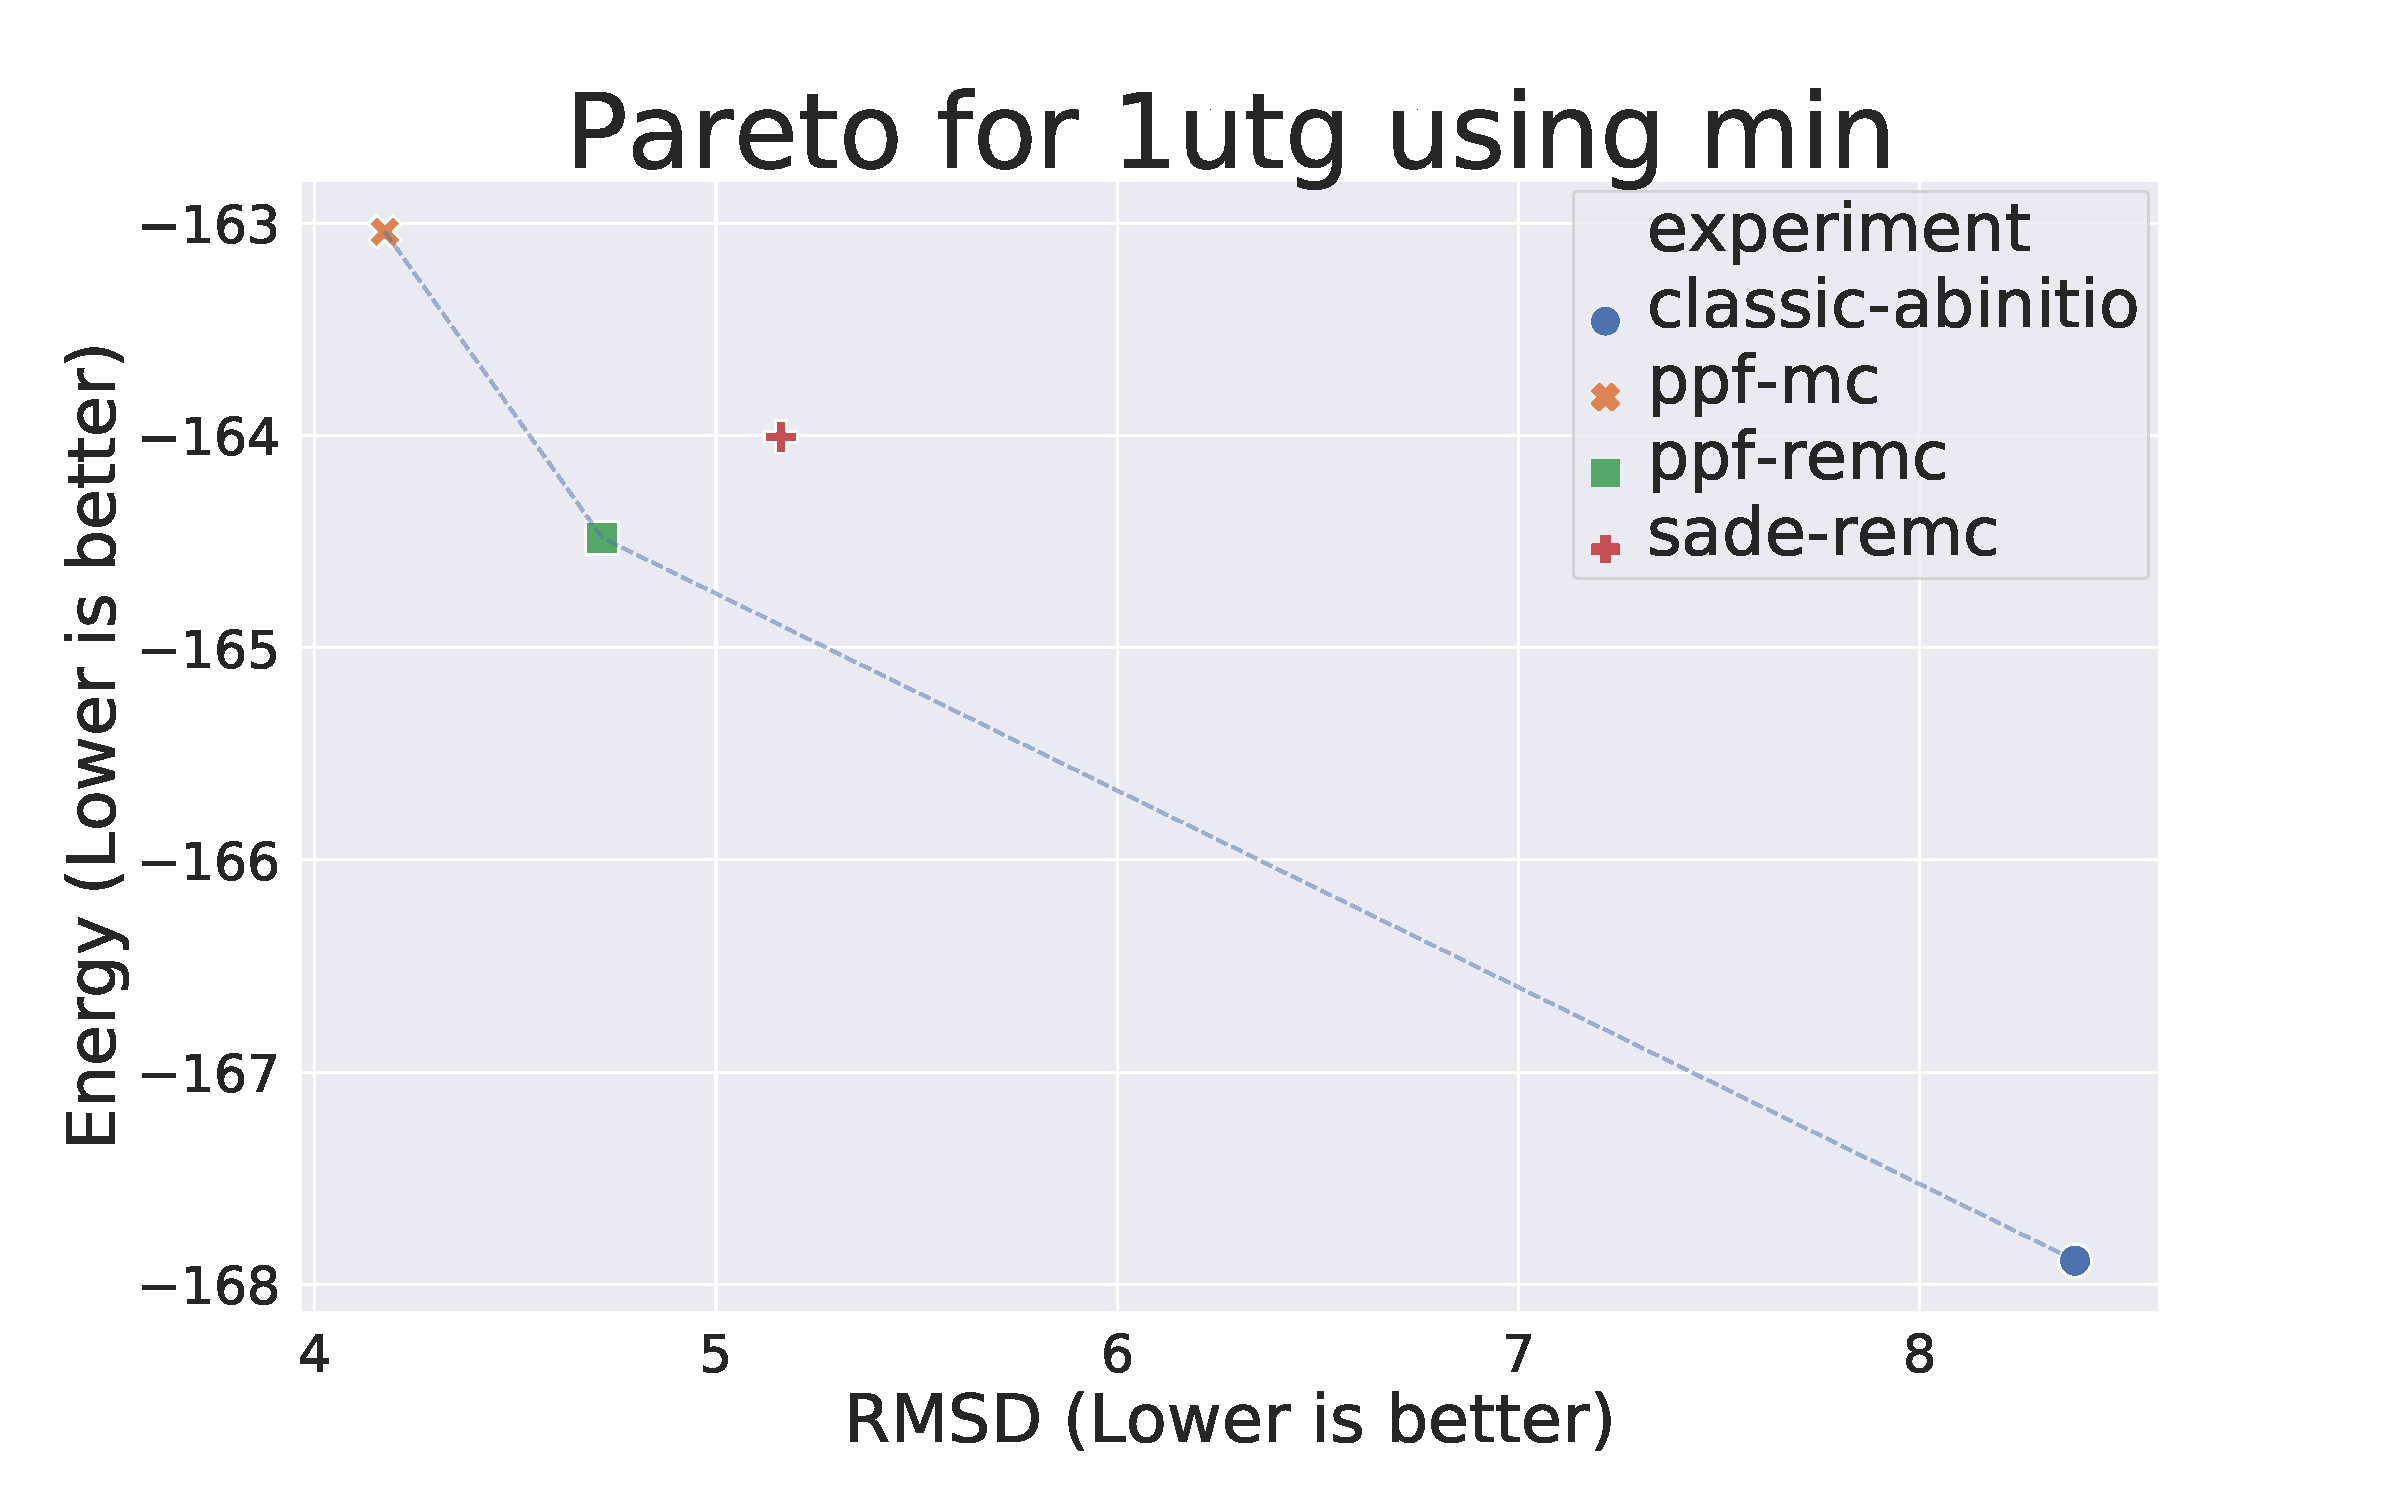
\includegraphics[width=1\linewidth]{Figuras/pareto/1utg_best_by_rmsd_min.pdf}
  \end{subfigure}
%
  \begin{subfigure}{0.49\linewidth}
    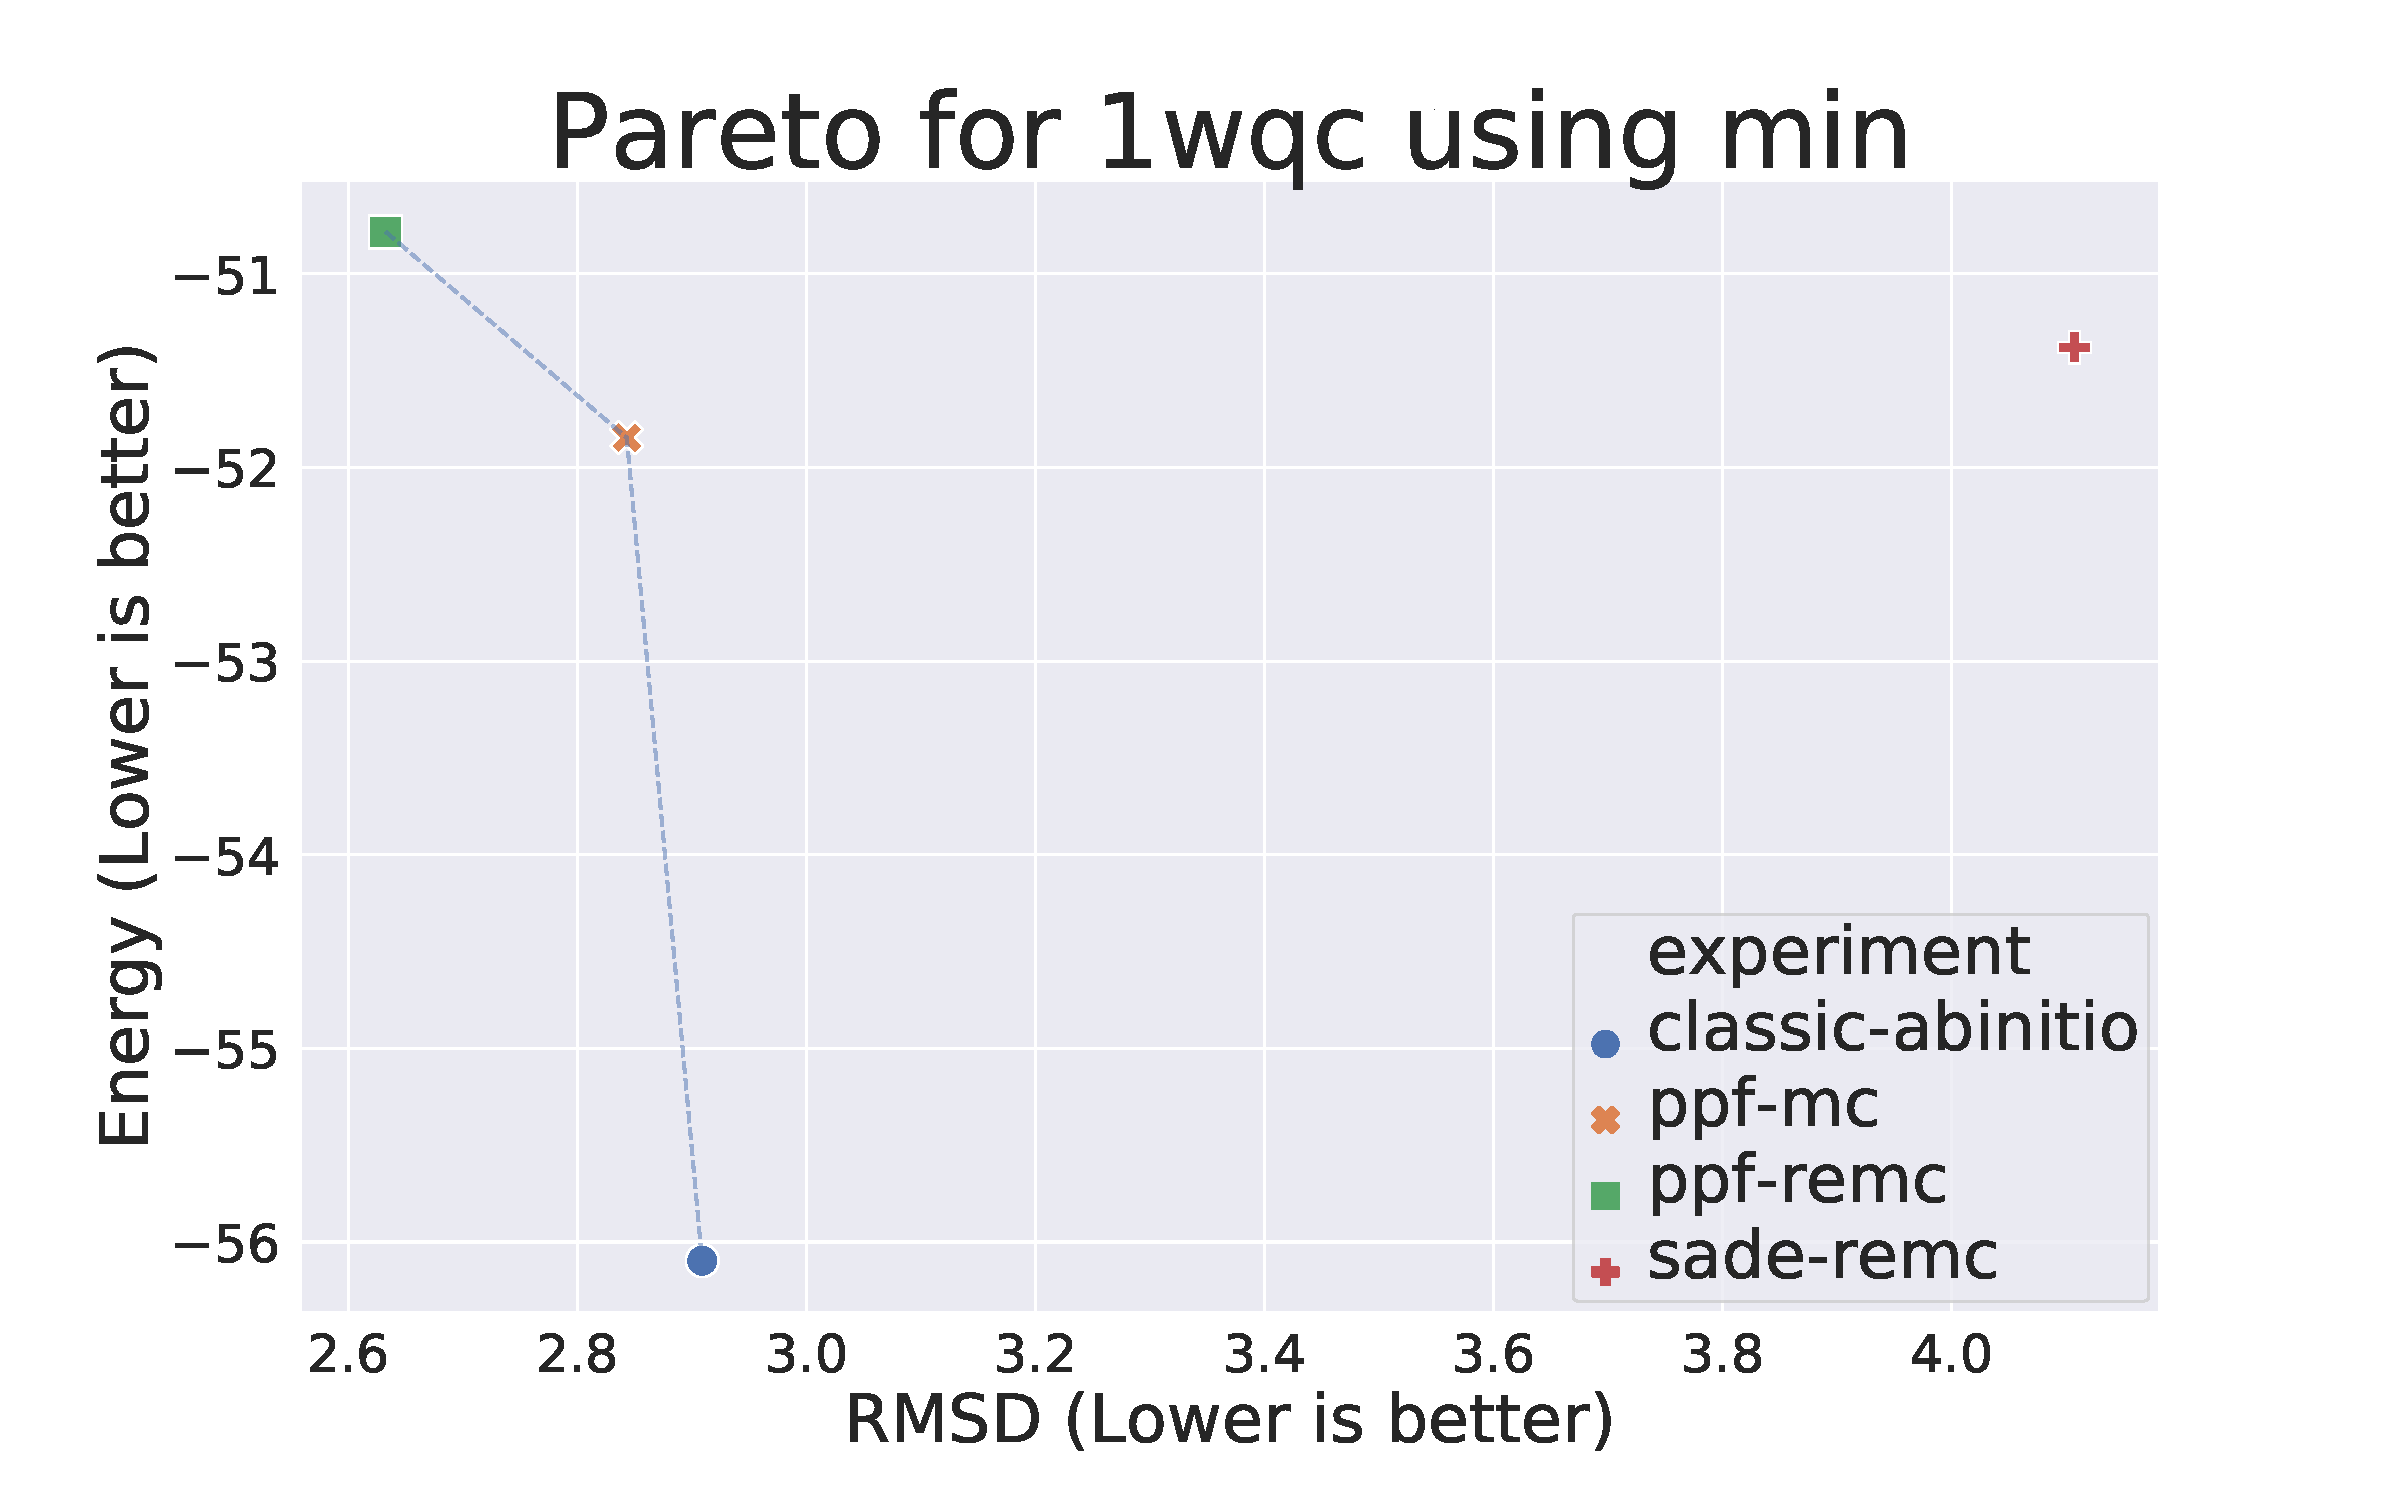
\includegraphics[width=1\linewidth]{Figuras/pareto/1wqc_best_by_rmsd_min.pdf}
  \end{subfigure}
%
  \begin{subfigure}{0.49\linewidth}
    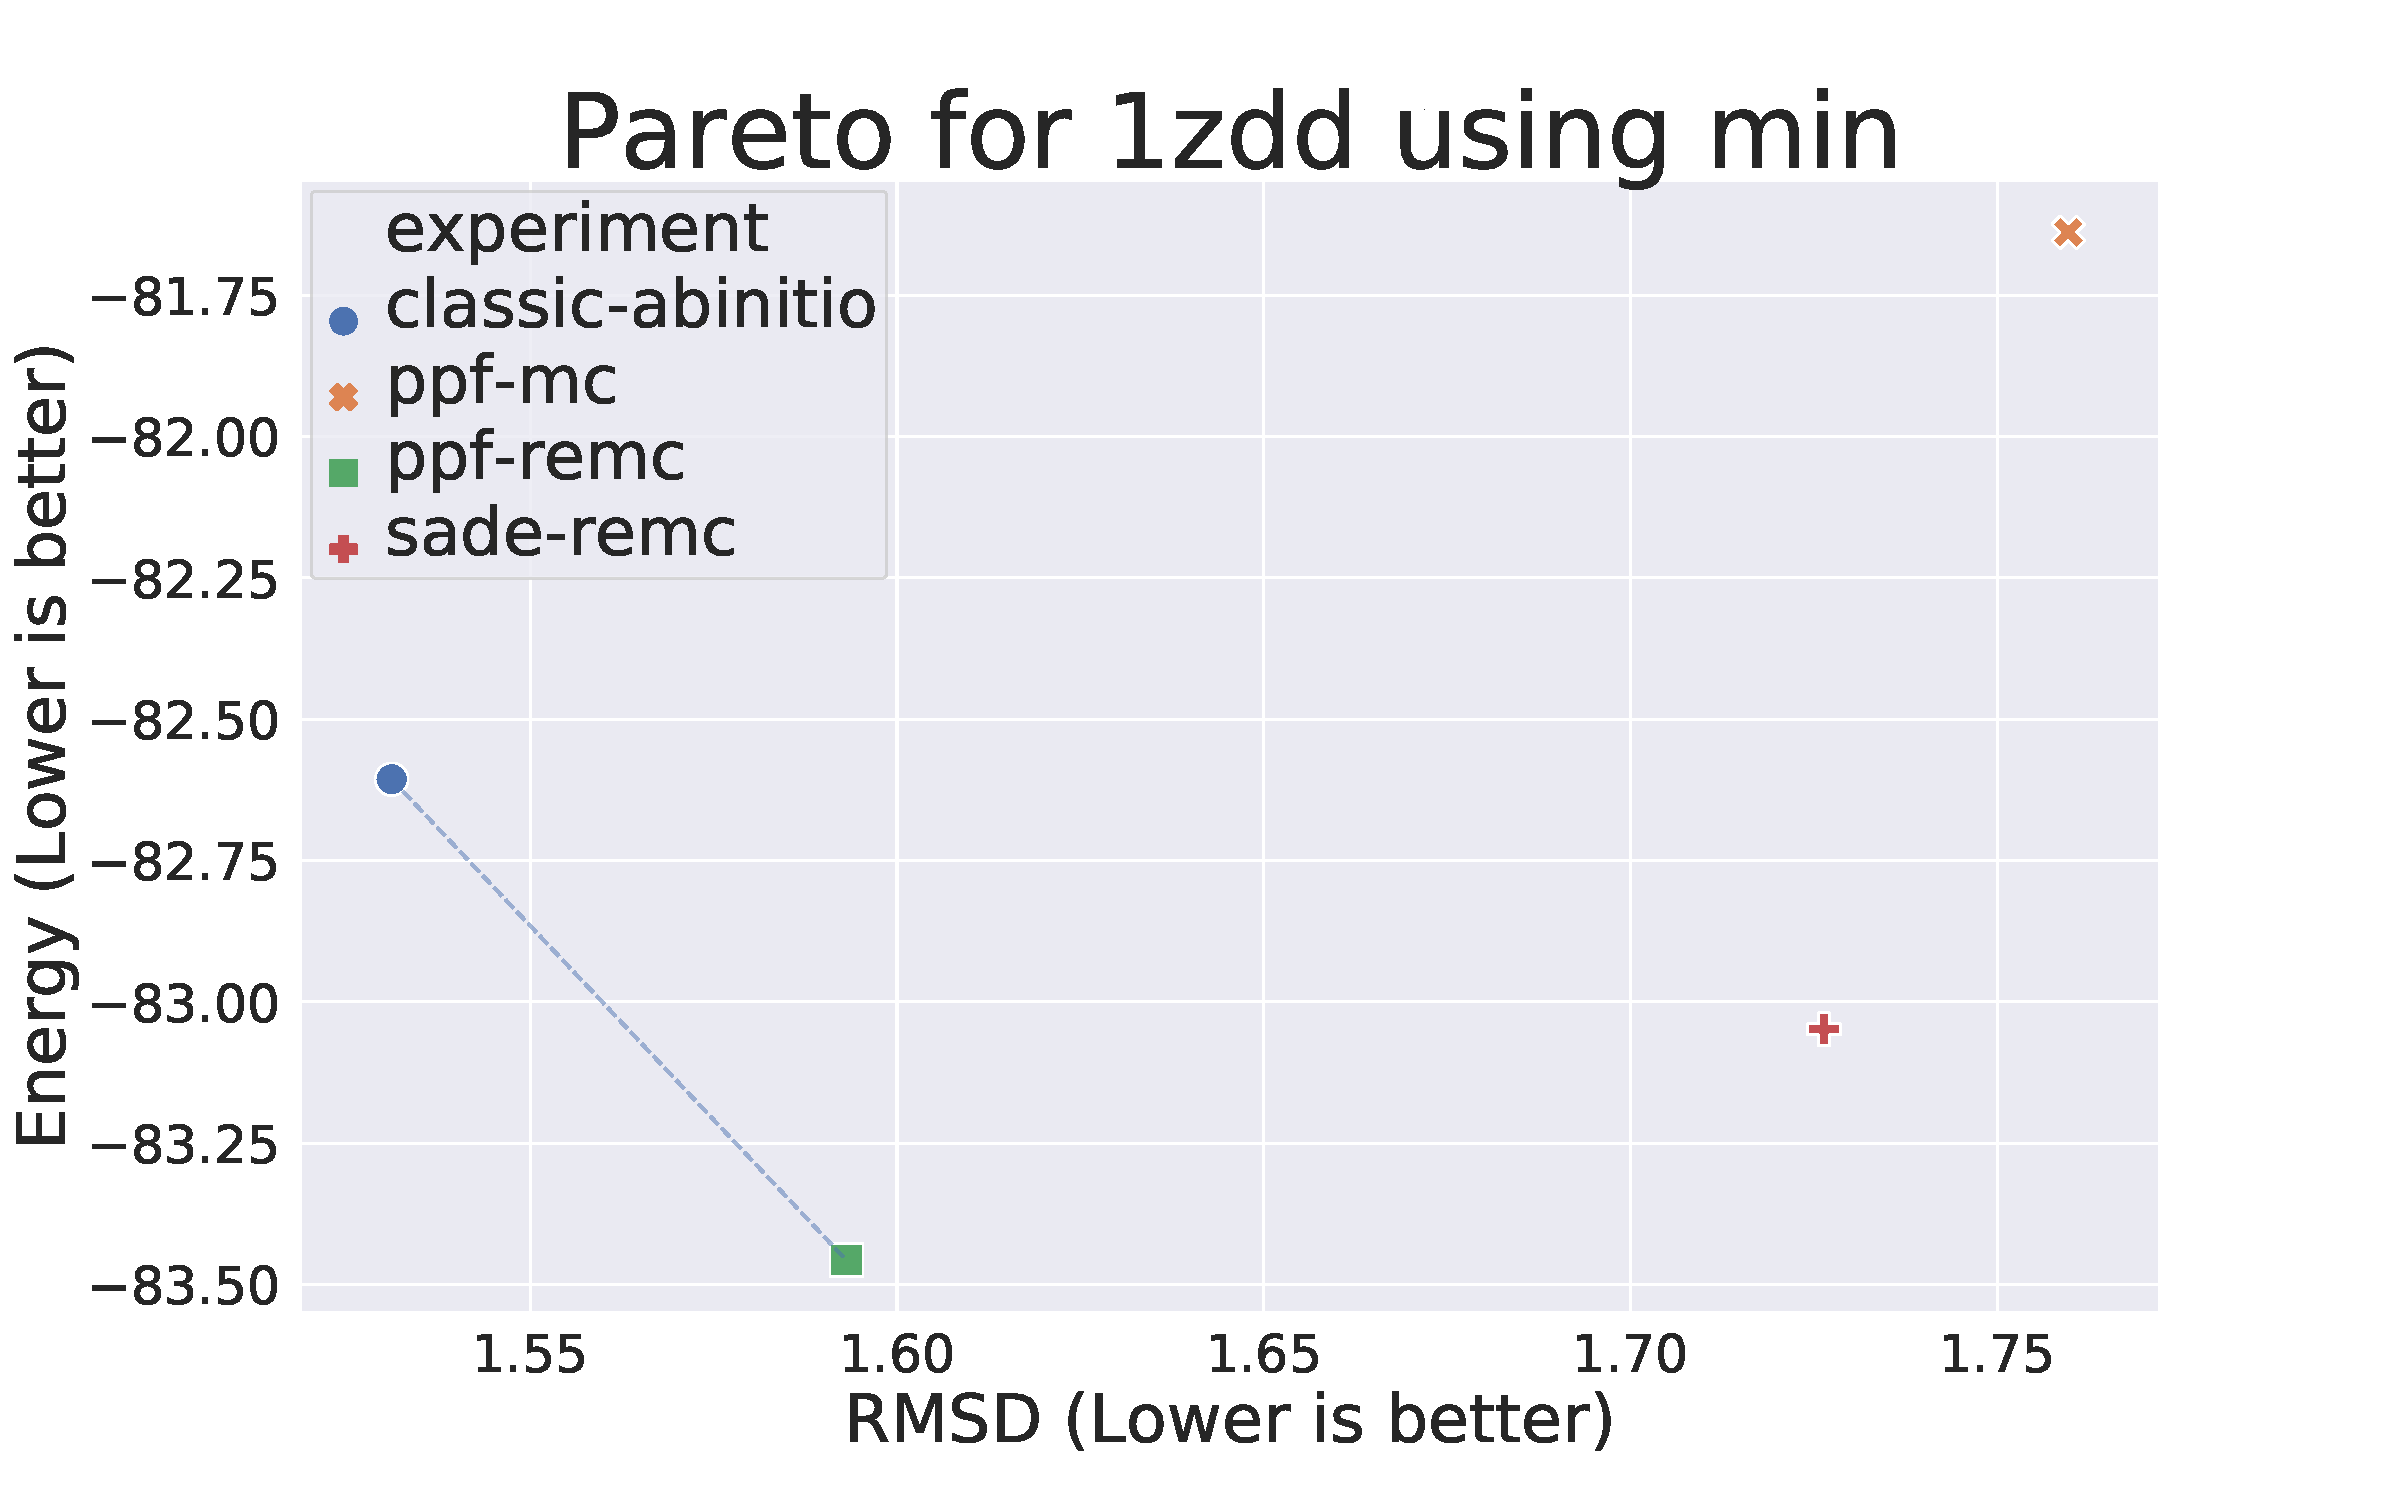
\includegraphics[width=1\linewidth]{Figuras/pareto/1zdd_best_by_rmsd_min.pdf}
  \end{subfigure}
%
  \begin{subfigure}{0.49\linewidth}
    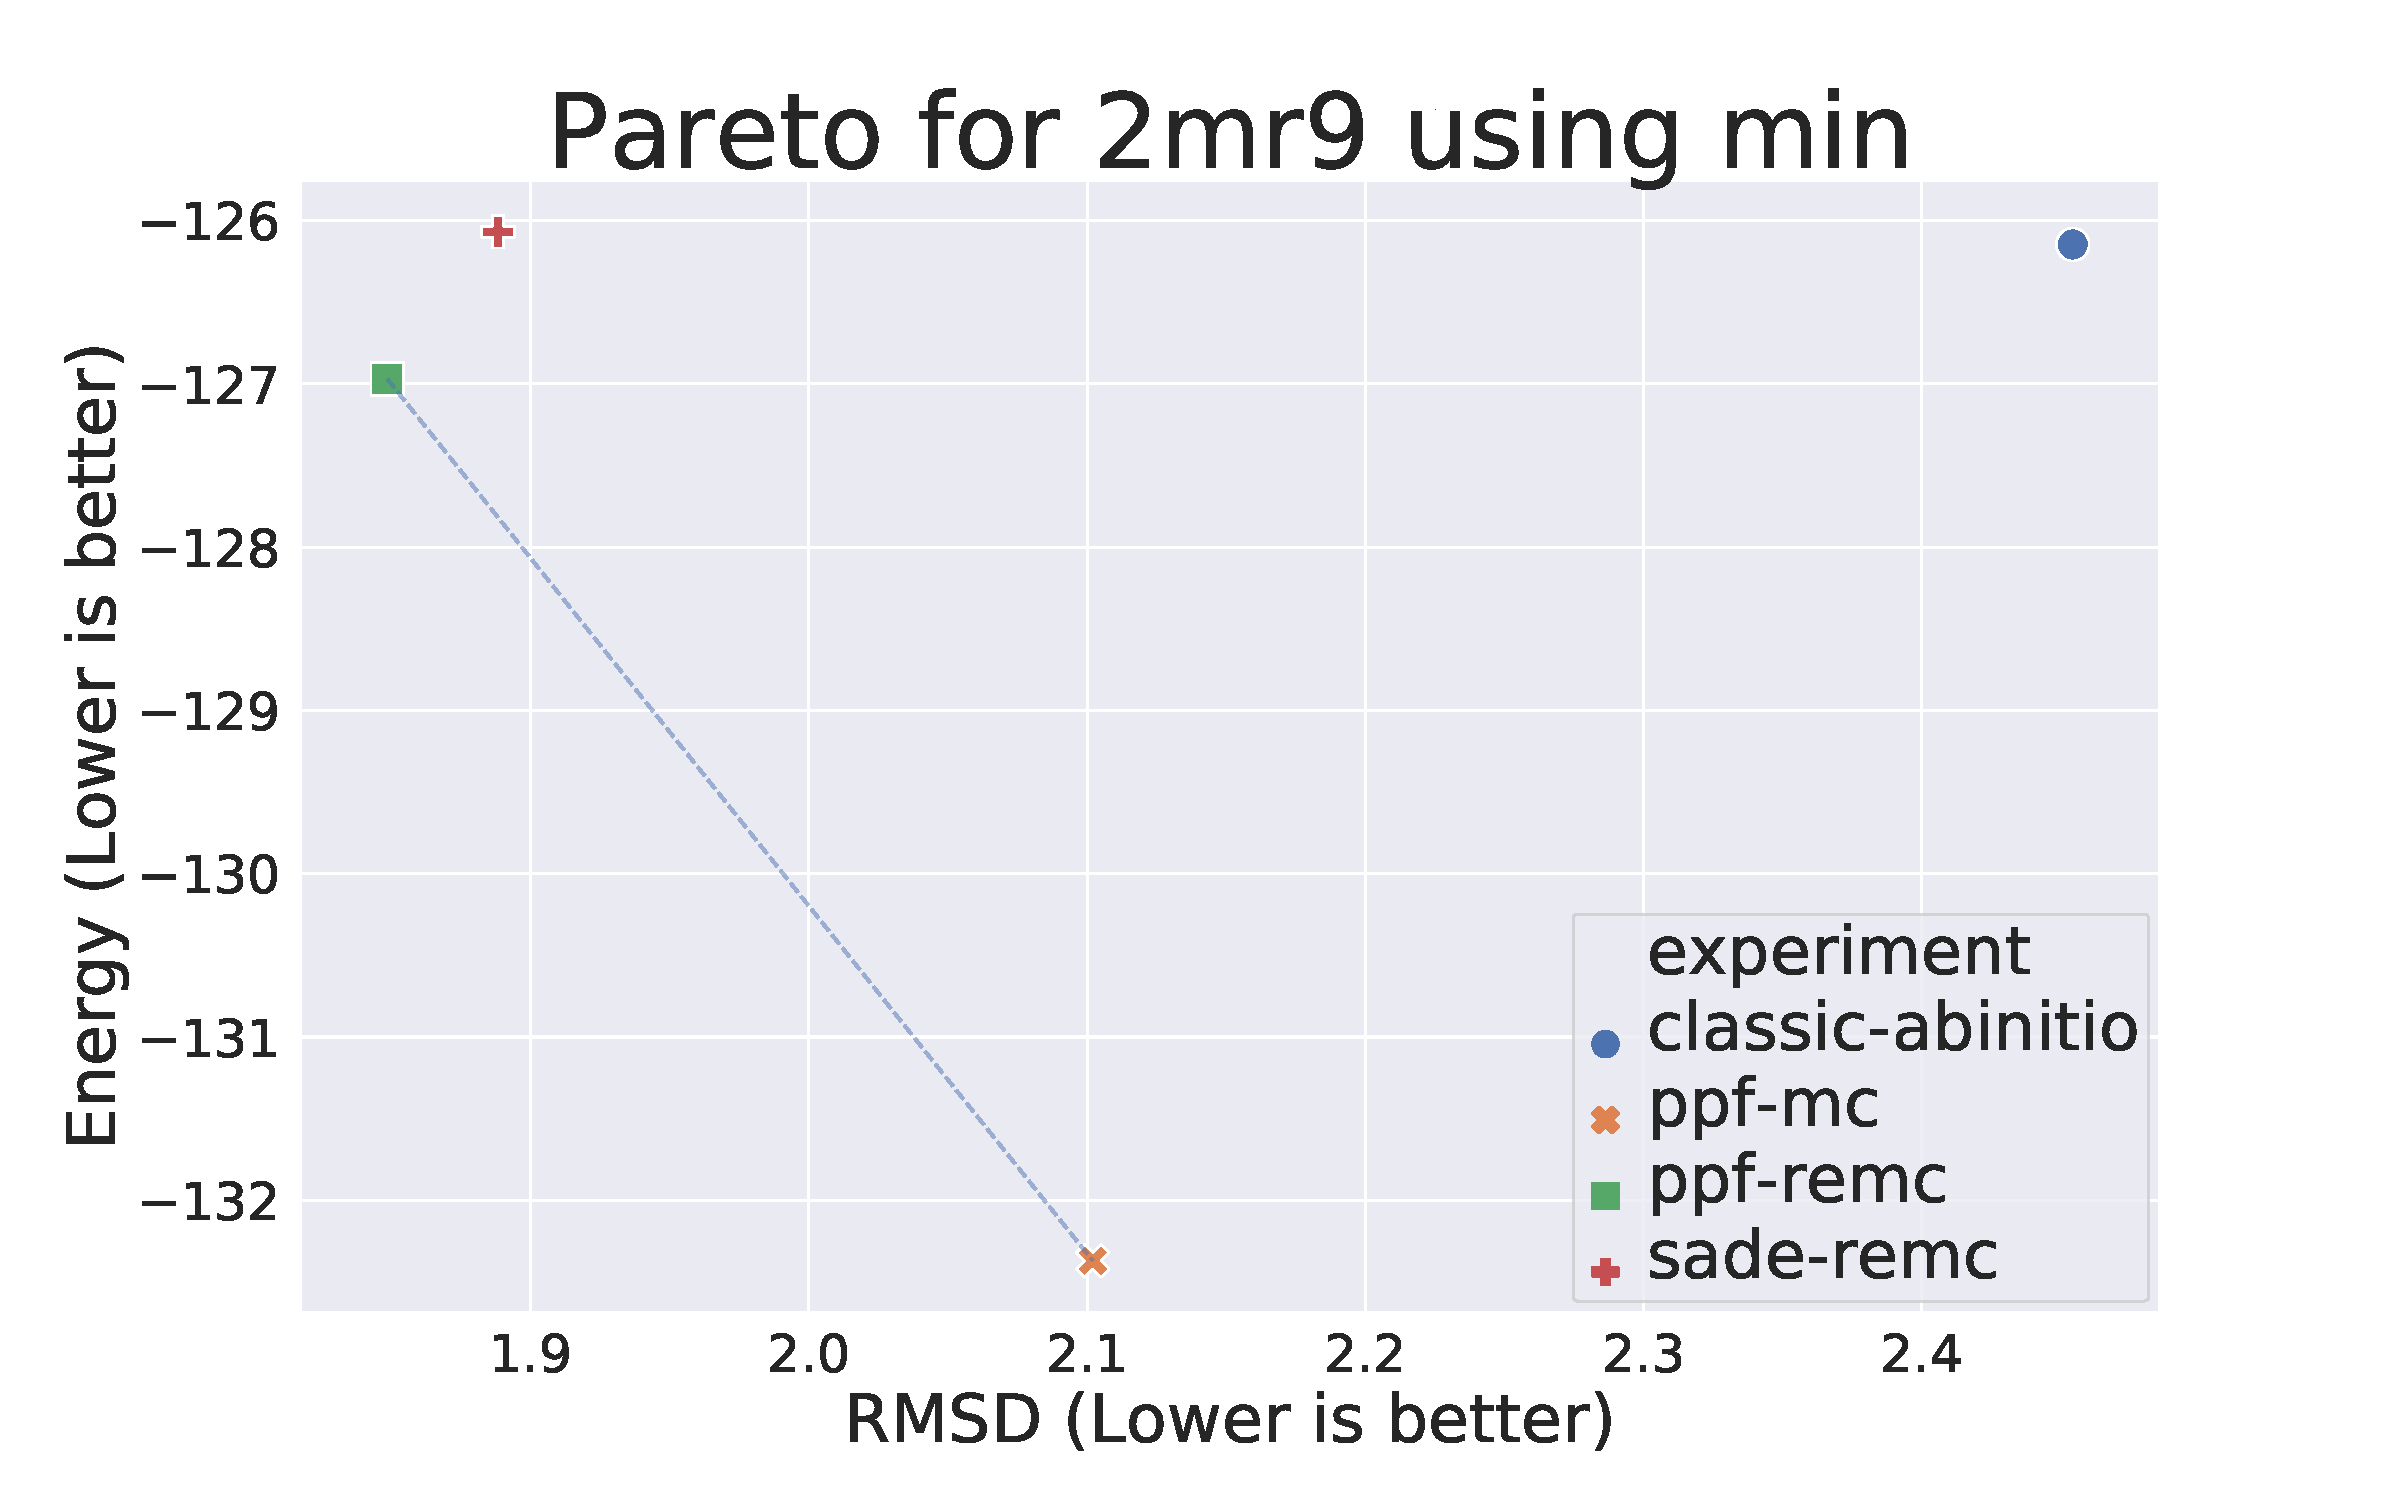
\includegraphics[width=1\linewidth]{Figuras/pareto/2mr9_best_by_rmsd_min.pdf}
  \end{subfigure}
  \caption{Pareto front of the methods using RMSD and Energy}
  \label{fig:pareto-front}
\end{figure}

The Pareto front for all 10 proteins is presented in
Figure~\ref{fig:pareto-front}. Each subfigure represents one protein.
The x-axis contains the RMSD and the y-axis contains the Energy. For proteins 1acw,
1ail, 1rop, 1zdd and 2mr9 there are two methods in the Pareto front. For
protein 1crn, there is one method which dominates all others. The remaining
proteins have three methods in the Pareto front, meaning that there is only one
method being dominated.

A summary of the which methods are present in the Pareto front is presented
in Table~\ref{tab:pareto-front-summary}. Column \textbf{Method} contains the method,
sorted by the number of times it appeared in the front. The second column,
\textbf{Proteins}, contains the proteins in which the method was in the Pareto front.
The third column, \textbf{Total}, contains the number of times the protein appeared in the
front.

\begin{table}
  \centering
  \begin{tabular}{r | r | c}
    Method    & Proteins                           & Total \\ \hline \hline
    ppf-remc  & 1acw 1crn 1l2y 1utg 1wqc 1zdd 2mr9 & 7     \\ \hline
    ppf-mc    & 1enh 1l2y 1rop 1utg 1wqc 2mr9      & 6     \\ \hline
    rosetta   & 1ail 1enh 1l2y 1utg 1wqc 1zdd      & 6     \\ \hline
    SADE-REMC & 1acw 1ail 1enh 1rop                & 4     \\
  \end{tabular}
  \caption{Summary of the method in the Pareto front}
  \label{tab:pareto-front-summary}
\end{table}

One of the proposed methods, ppf-remc, appeared in the Pareto front for $7$ out of 
$10$ proteins. Both rosetta and ppf-mc appeared in $6$ proteins. Finally,
SADE-REMC appeared only in $4$. On 1acw, 1crn, 1rop and 2mr9 at least one of the
proposed methods appeared in the front while rosetta did not. The converse,
rosetta being in the front while none of the proposed methods were, happened
only for 1ail.

Considering these observations, the two proposed methods and rosetta have a
similar performance regarding the Pareto front. However, rosetta was only
able to dominate the two proposed method in one occasion. Meanwhile, rosetta was
dominated in $4$.
\textcolor{red}{
Moreso, with the exception of 1zdd, the proposed methods
always appeared to the left of rosetta in the pareto front, indicating
a lower RMSD.
}
Taking this into account, it can be concluded that the two
proposed methods are able to give good conformations with varying properties
where an human expert can choose from.

\section{Convergence and Diversity Analysis}
\label{sec:convergence-analysis}

In this Section, the behaviour of the two proposed methods is analysed. The
analysis is divided in a genotipic and a phenotypic convergence analysis. The
genotipic analysis is related to how diverse the conformations are. This is
measured as the mean pairwise RMSD between all $100$ conformations in the
population. The phenotypic analysis is made considering both the energy of
the best individual and the mean energy in the population. Considering that
$50$ independent runs of each method were ran, the data to be analysed is
the mean over all runs. That is, the data on the following graphs are
the mean of mean pairwise rmsd, the mean of the best individual and the mean
of the mean population energy. Moreover, there are $20$ convergence graphs. As such,
a few select proteins are selected for analysis.
Appendix~\ref{appendix:convergence-plots} contains the plots for all 10
proteins.

\begin{figure}[ht]
  \begin{subfigure}{0.499\linewidth}
    \centering
    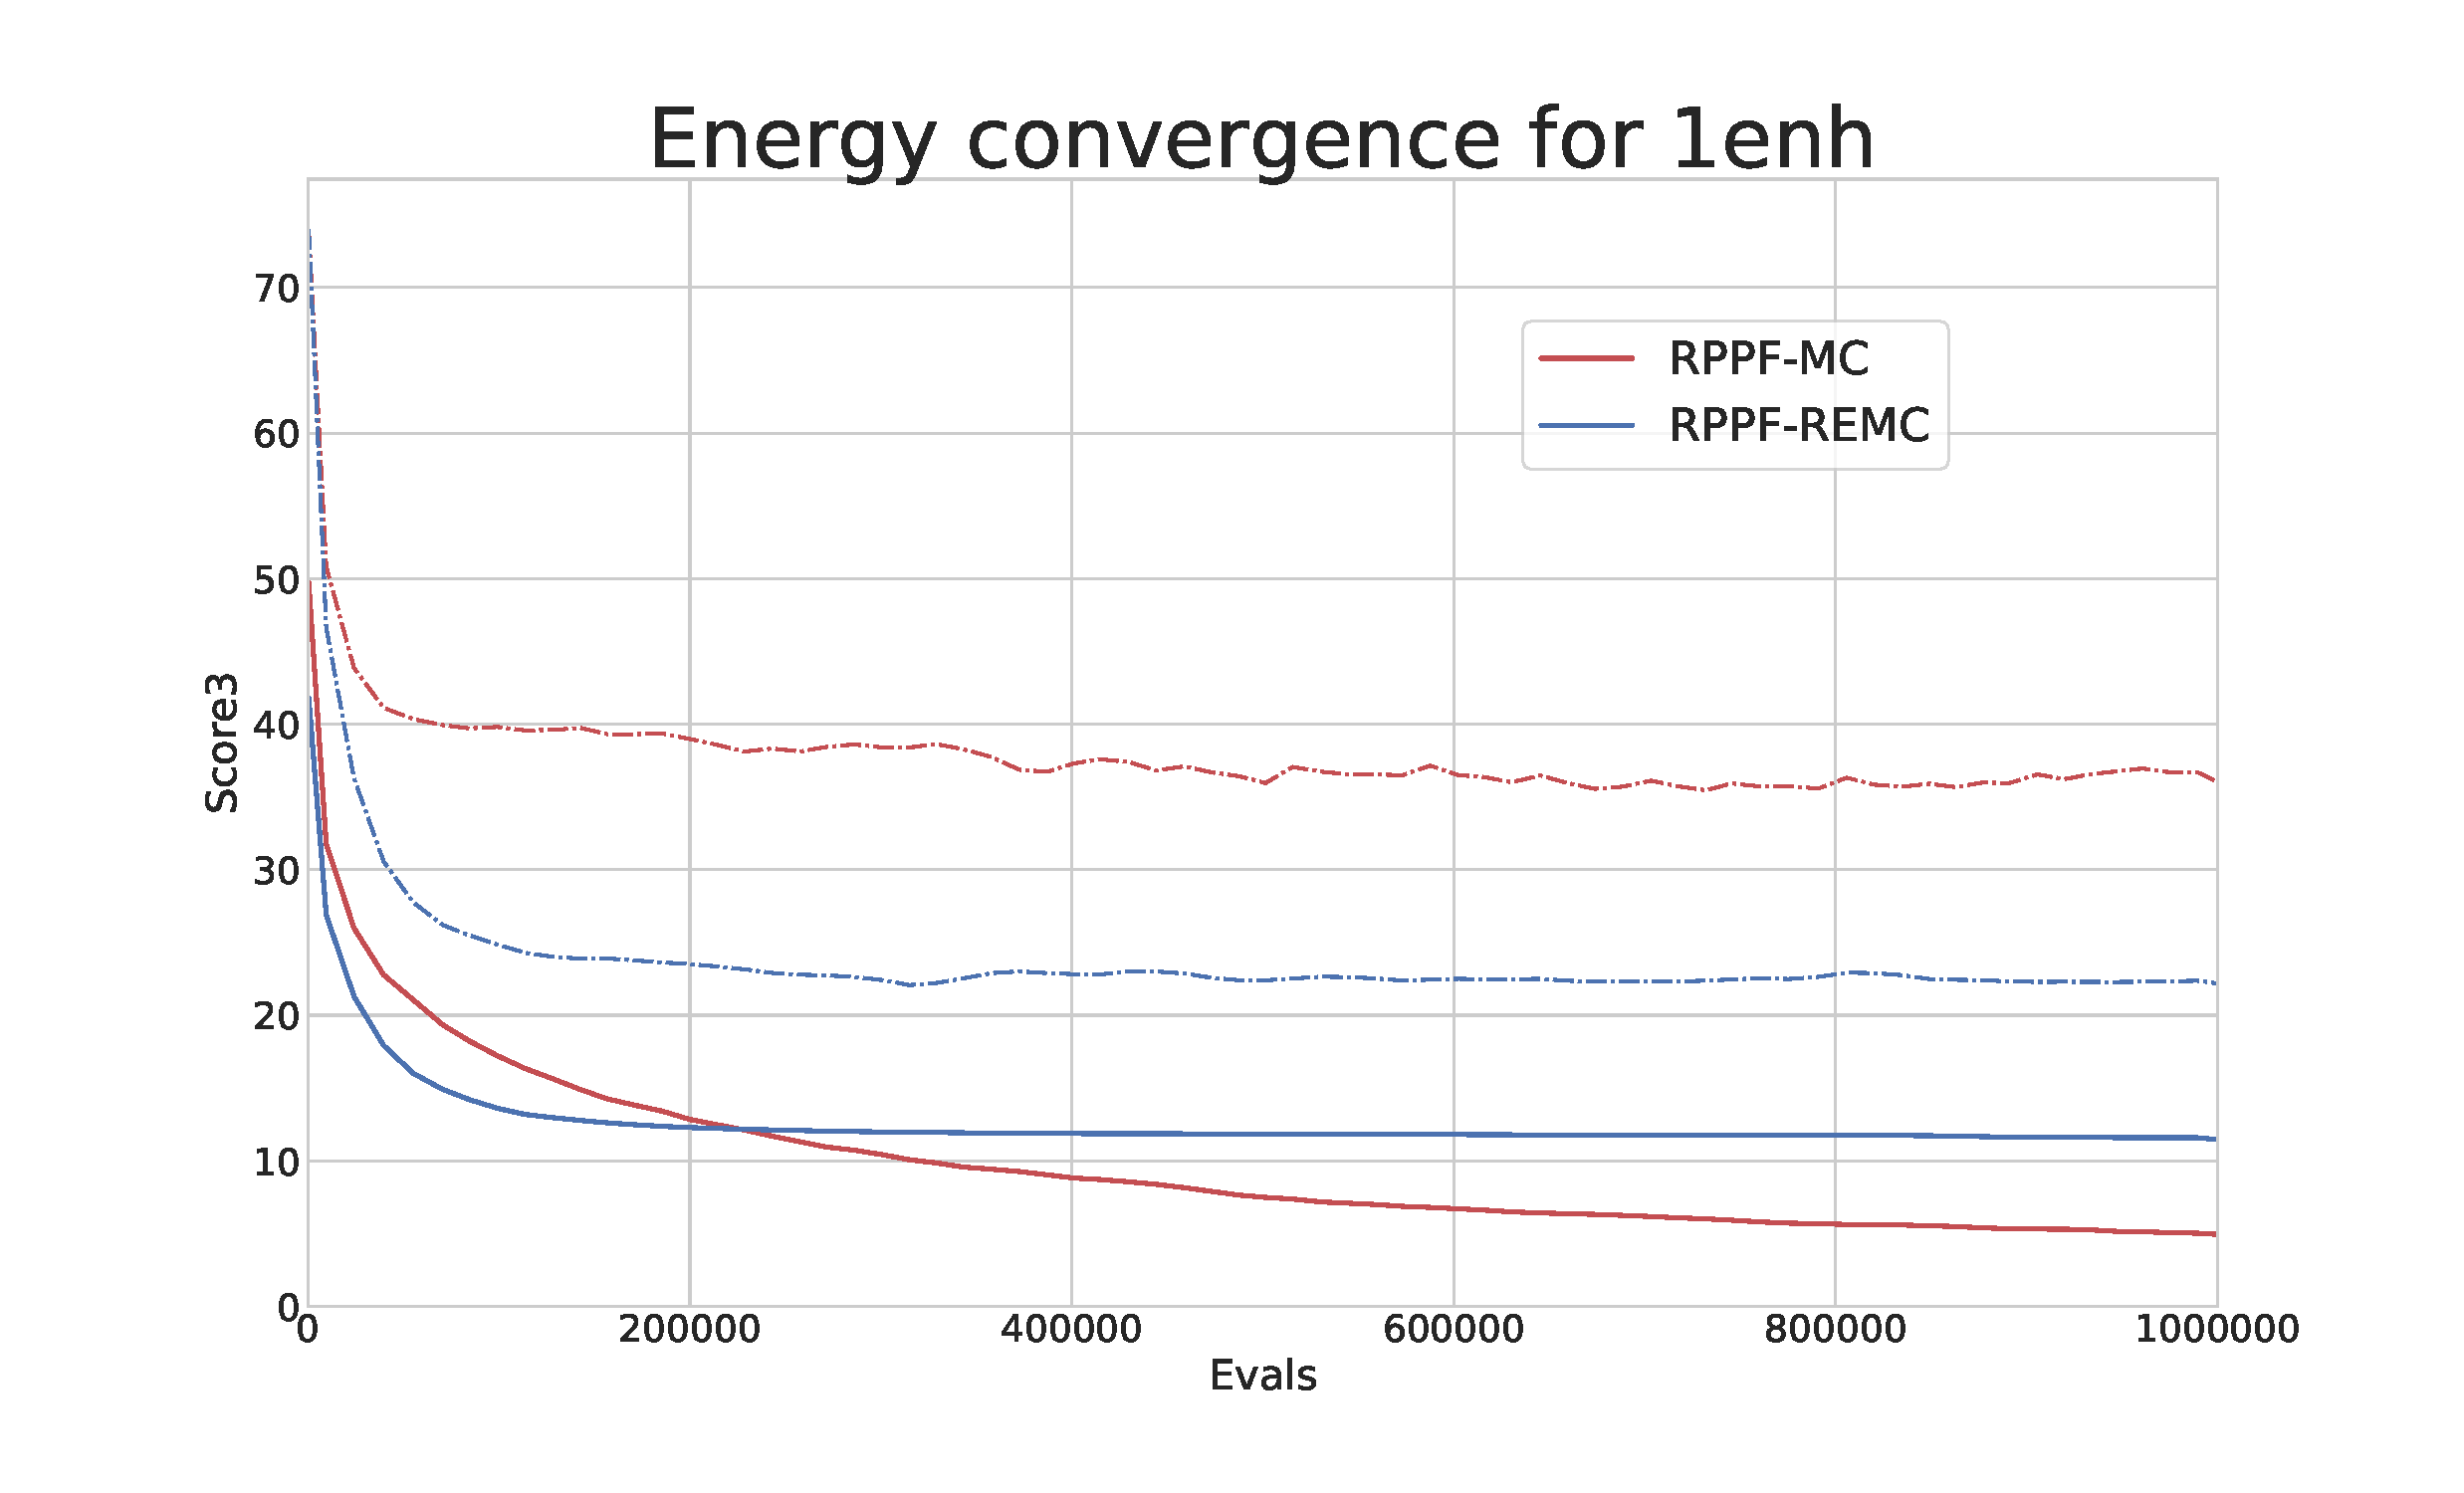
\includegraphics[width=1\linewidth]{Figuras/plots/energy_convergence/energy_convergence_1enh.pdf}
    \caption{1enh}
    \label{fig:1enh-energy-convergence}
  \end{subfigure}
%
  \begin{subfigure}{0.499\linewidth}
    \centering
    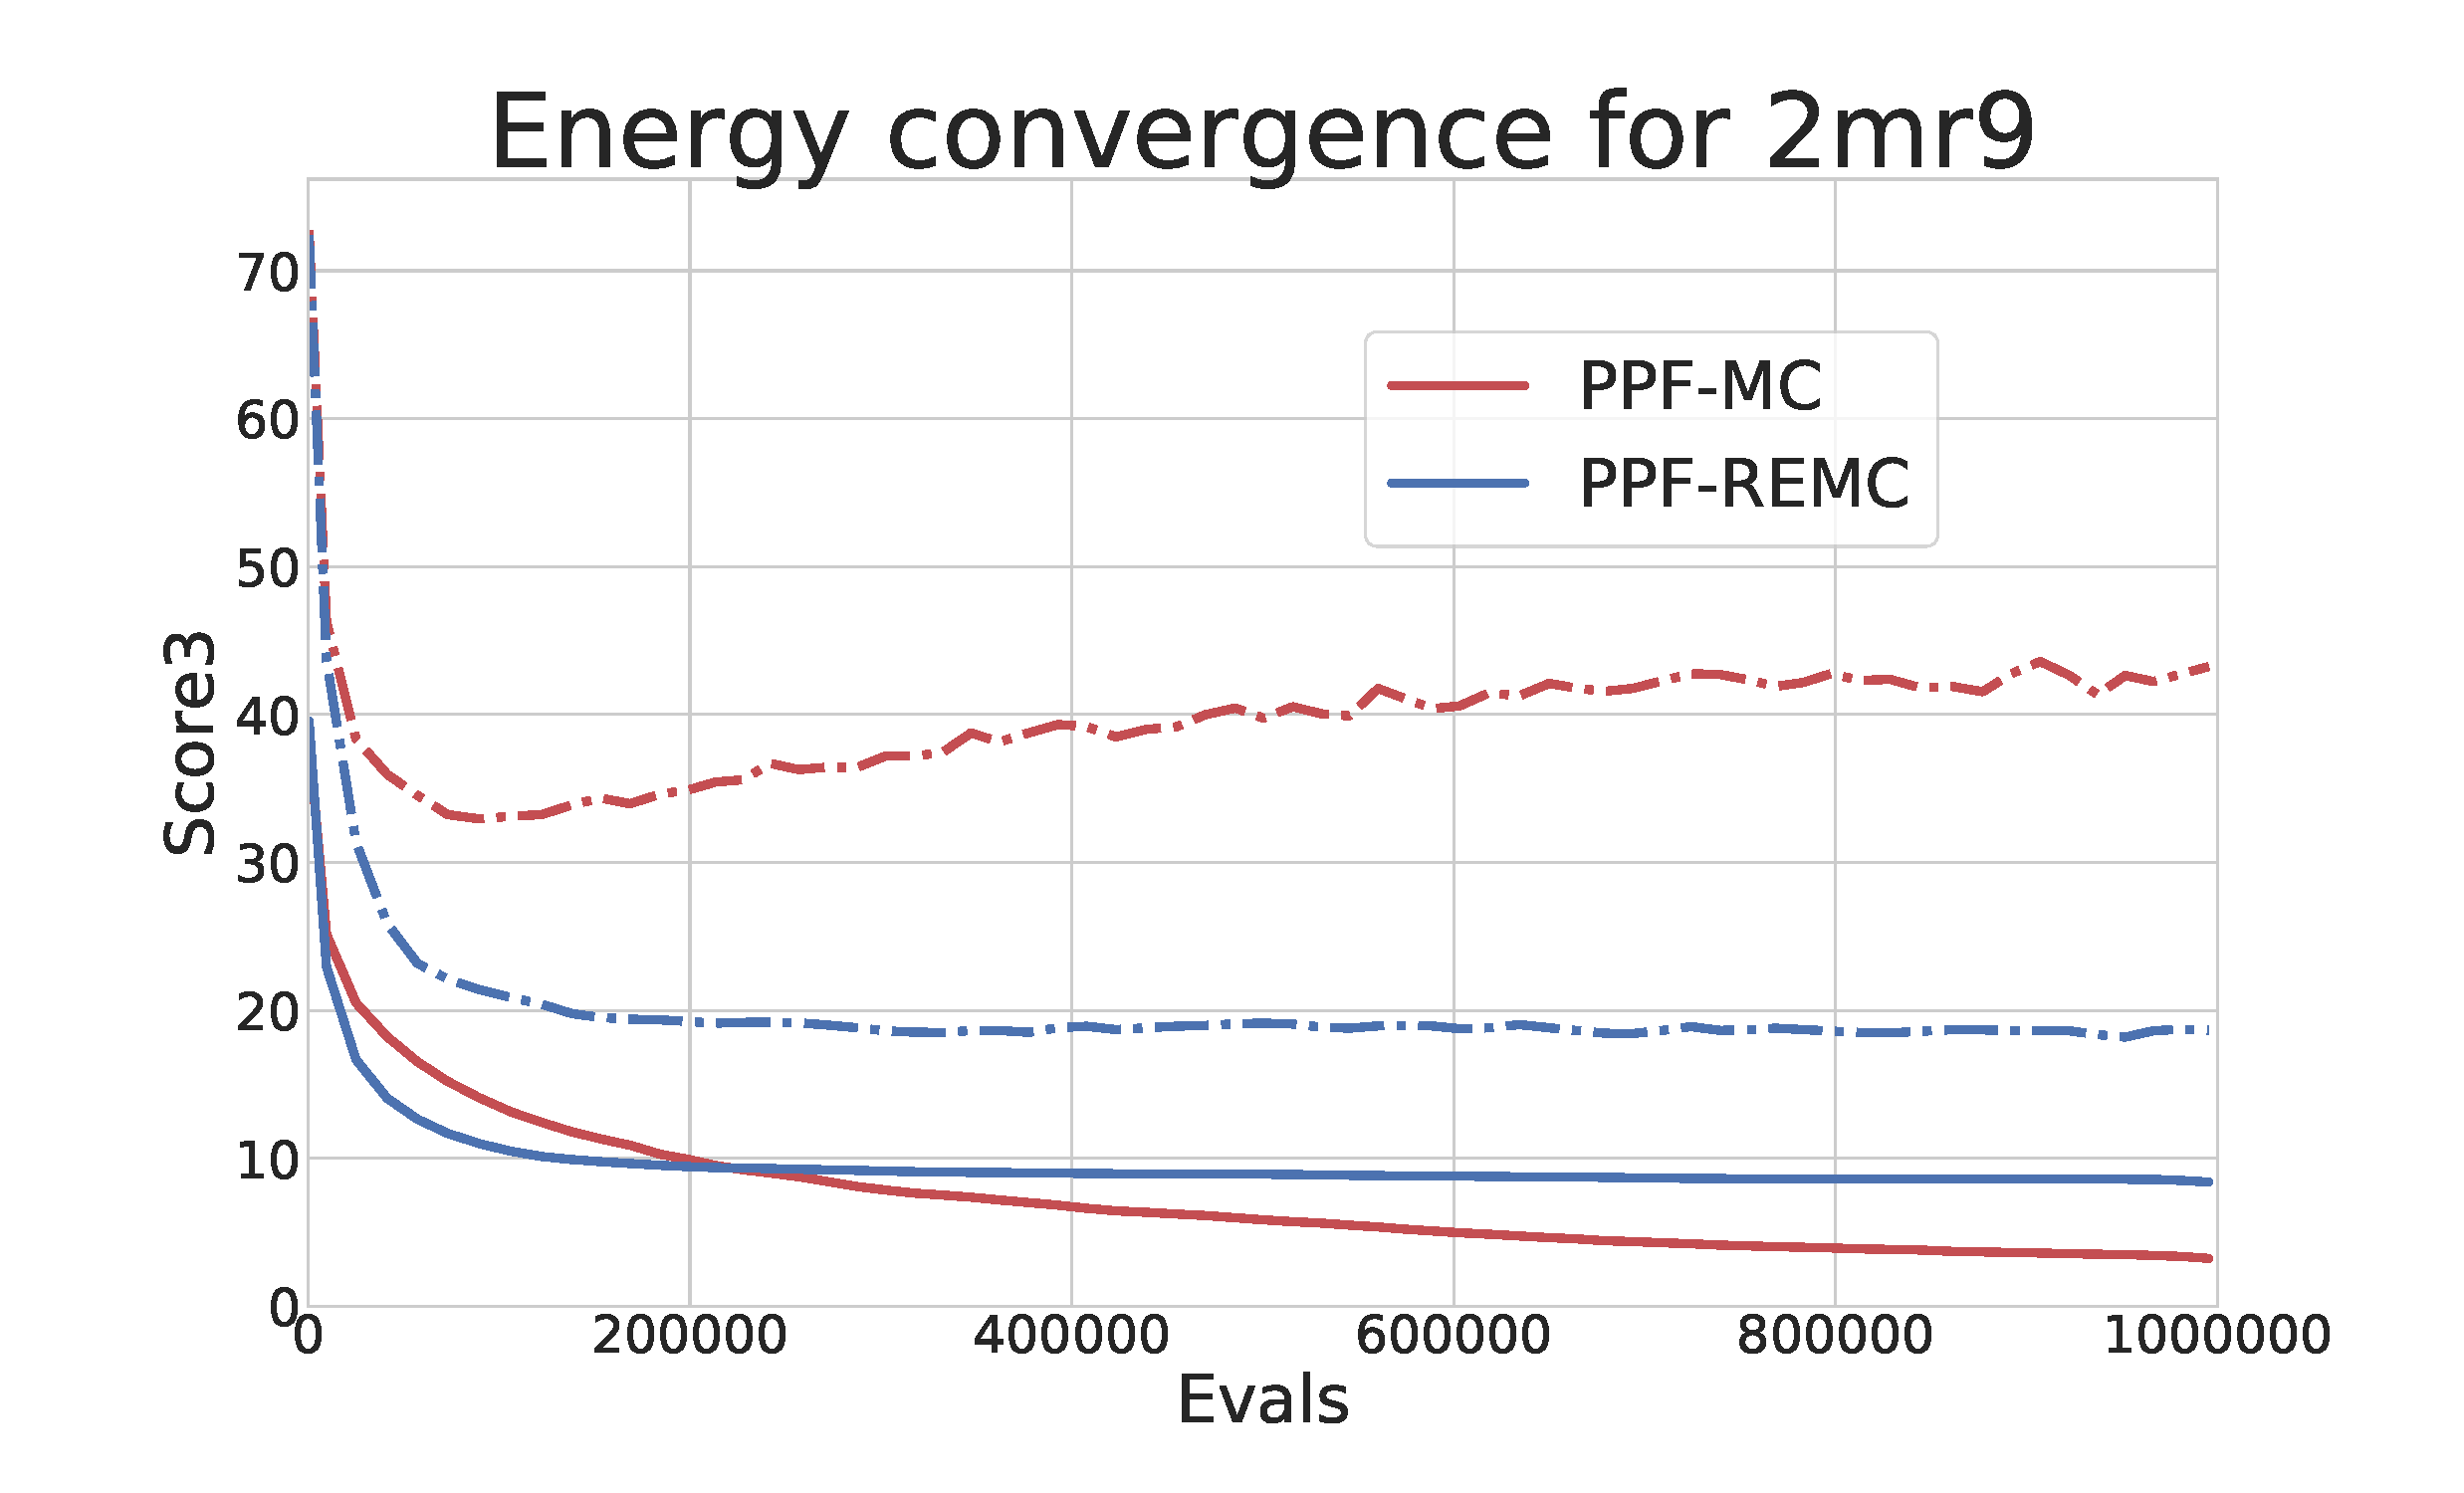
\includegraphics[width=1\linewidth]{Figuras/plots/energy_convergence/energy_convergence_2mr9.pdf}
    \caption{2mr9}
    \label{fig:2mr9-energy-convergence}
  \end{subfigure}
  \caption{The best energy and average energy for proteins 1enh and 2mr9. The
  continuous line represents the best energy. The dashed line represents the
  average of the population. The X Axis represents the function evaluations and
  the Y Axis indicates the value of the \texttt{score3} energy function being
  optimized.}
  \label{fig:energy-convergence-1enh-2mr9}
\end{figure}

In Figure~\ref{fig:energy-convergence-1enh-2mr9} the behaviour of the two
proposed methods is displayed. Protein 1enh was chosen as a representative
of standard behaviour.
There are seven other proteins with the same overall characteristics. That is,
the conclusions drawn from 1enh are also found in the other proteins.
In blue, it is possible to see that ppf-remc has a very fast
convergence during the first 50 thousand function evaluations. After that, it
quickly comes down to a halt in convergence. This, is a classic symptom of
premature convergence. With the dashed lines, representing the average of the
population, the same overall behaviour is observable. It is worth noting that
the line is not smooth. The small "bumps" presents are caused by FFI, which
can disrupt the mean energy of the population. For ppf-mc the convergence
starts slower than for ppf-remc, however, the best energy keeps improving
for more than three fifths of the available budget of functions evaluations.
Furthermore, on the dashed line representing the average energy, it is possible
to see that the the average improved over time as well.

When comparing ppf-mc and ppf-remc, by looking at the best energy of the two
methods, there is a lead for ppf-remc during the first 50 thousand function
evaluations. However, eventually ppf-mc achieves a best result and keeps
improving for the bigger part of the process. For all 10 proteins this can be
observed. Furthermore, when considering the average, ppf-remc had the best
results in all cases.

Two of the proteins had an increase of the average populational energy over time.
This happened only for protein 2mr9 with ppf-mc. This is the reason that this
protein was selected for analysis. The best energy for both methods and the
average energy for rppc-remc shows the same behavior as 1enh. However, the
average energy for ppf-mc, after approximately 70 thousand function iterations
starts to increase until reaching a point of equilibrium at 700 thousand
function evaluations, where it starts relatively stable. This behaviour is
caused by FFI. FFI has a $2\%$ chance of being applied before any other operator
is applied. For this particular protein, FFI managed to destroy more information
than the MC fragment insertion could recover.

A similar situation happened on 1l2y, however, for the best energy for
rppc-remc. There, the best energy eventually started to increase and continued
to steadily decrease until the optimization stopped. This can also be explained
by FFI.

\begin{figure}[ht]
  \begin{subfigure}{0.499\linewidth}
    \centering
    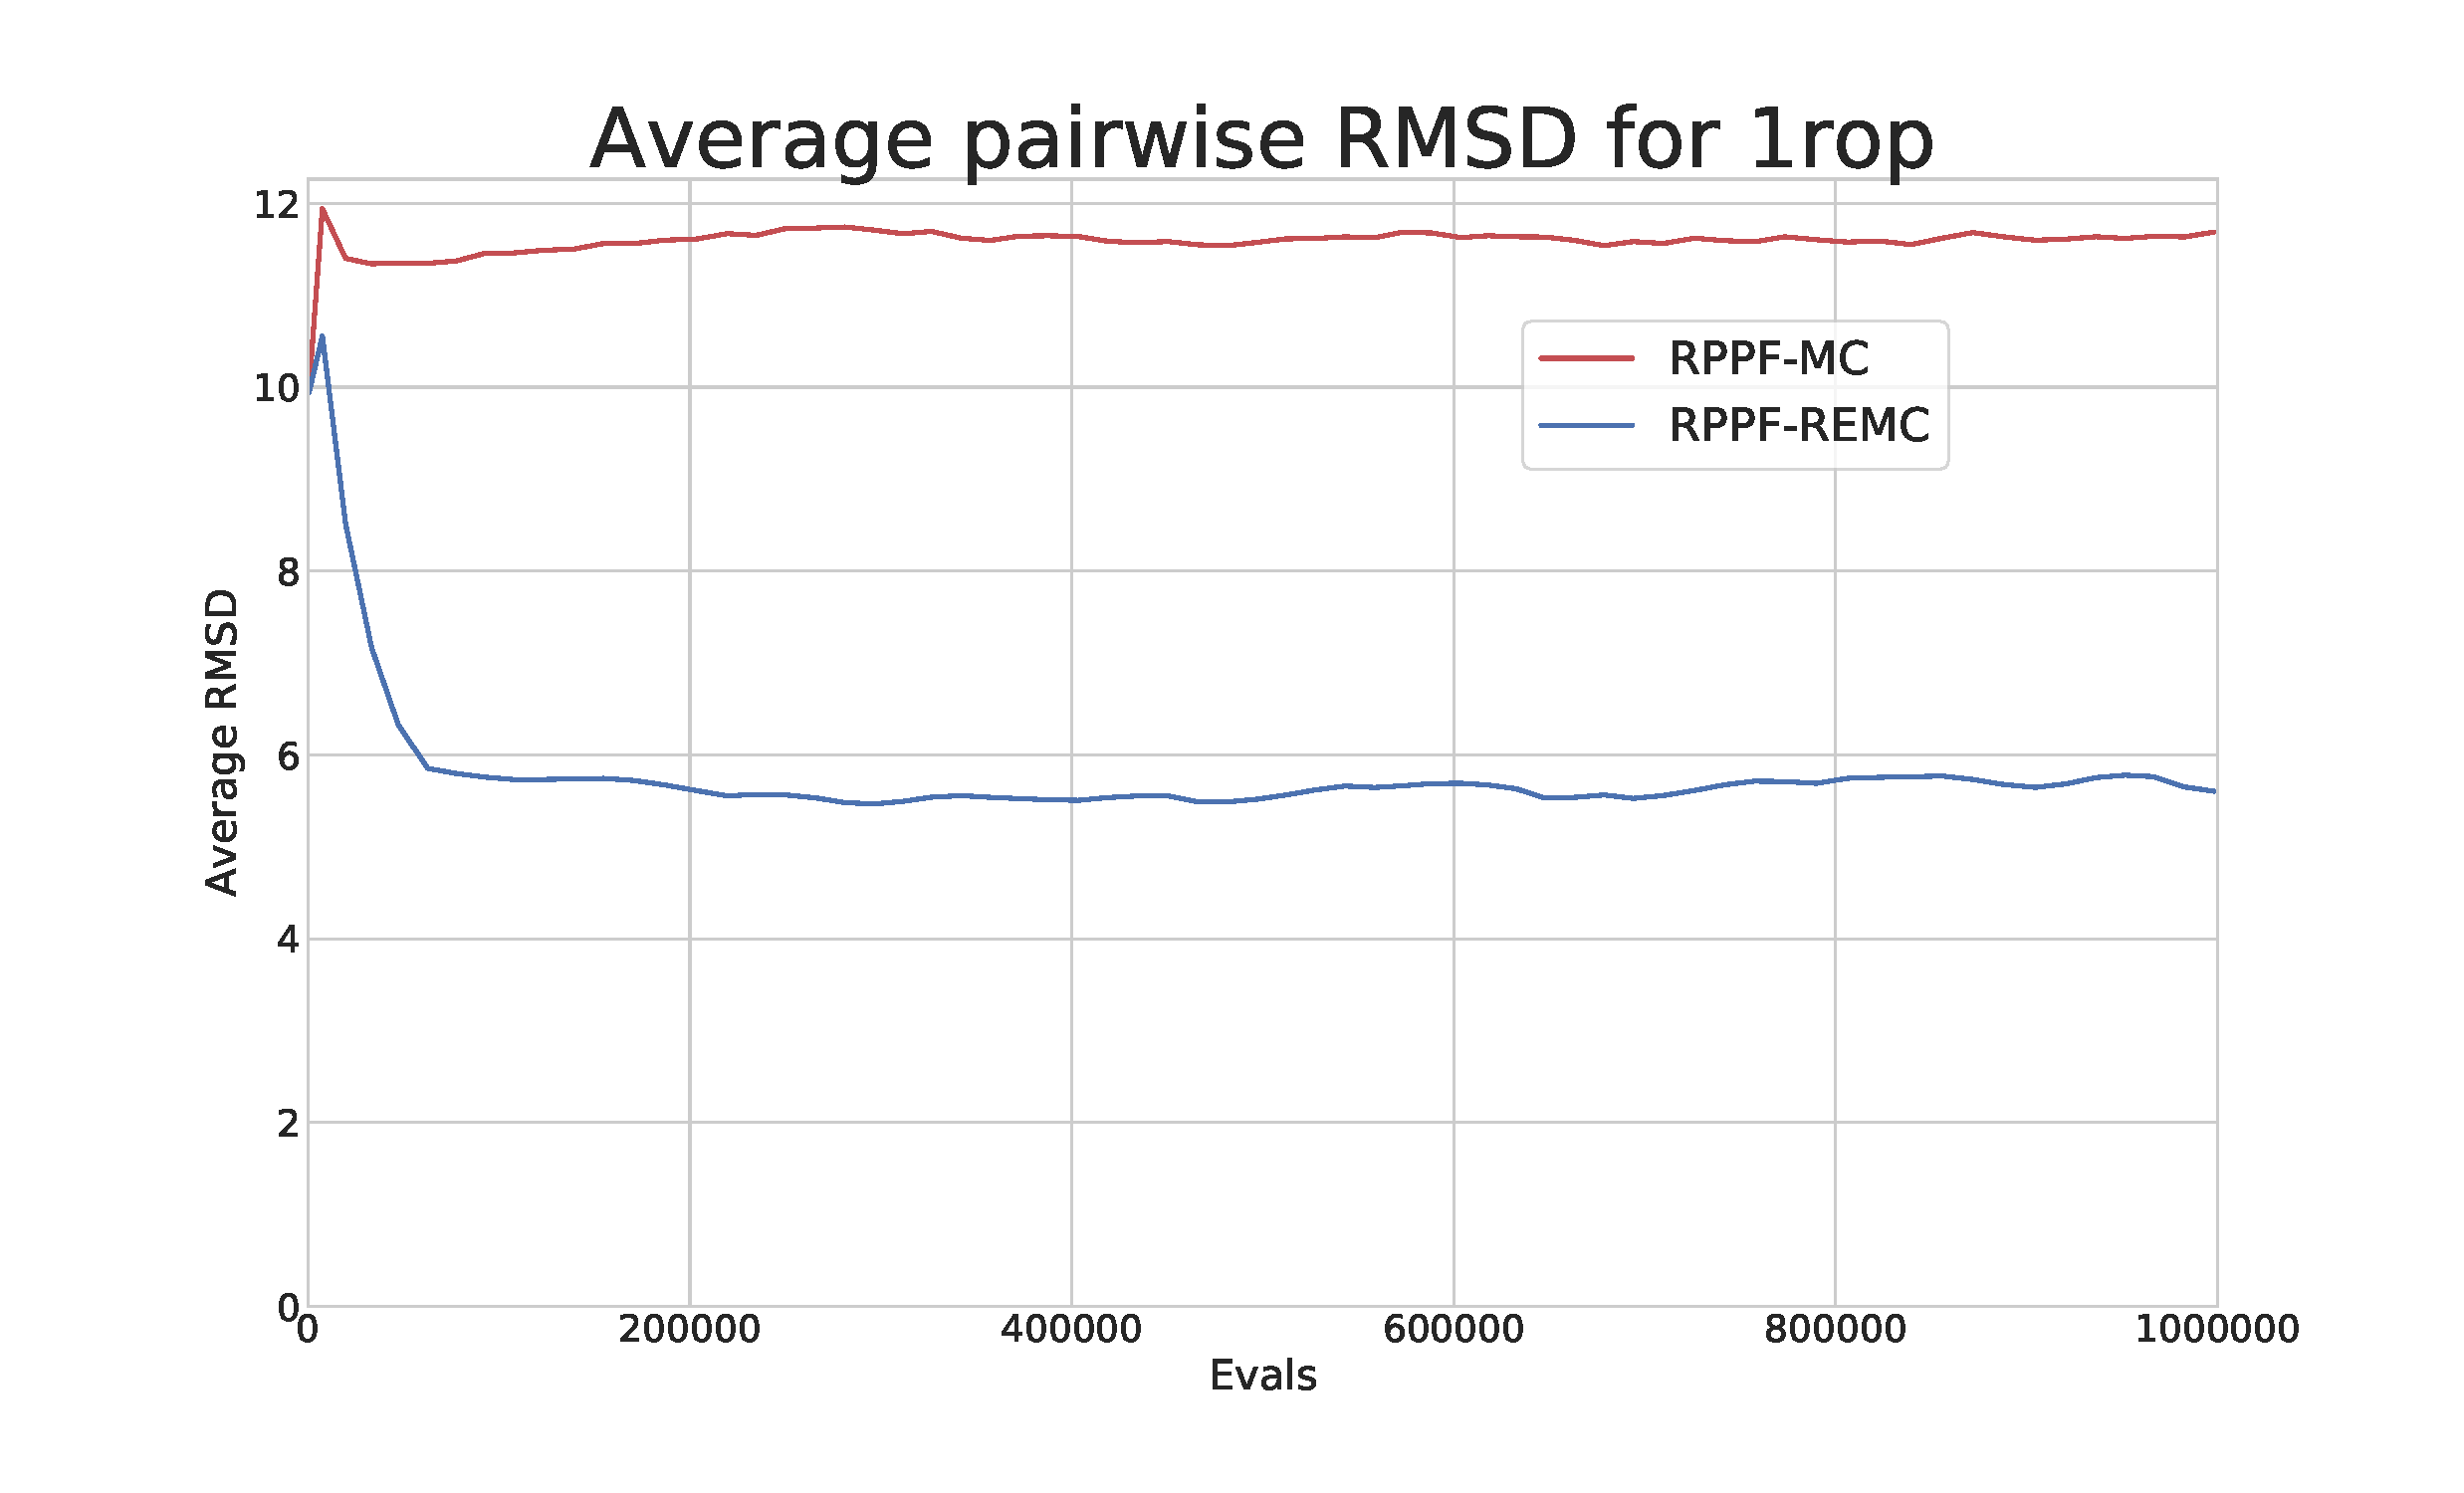
\includegraphics[width=1\linewidth]{Figuras/plots/rmsd_convergence/avg_rmsd_1rop.pdf}
    \caption{1rop}
    \label{fig:1rop-rmsd-convergence}
  \end{subfigure}
%
  \begin{subfigure}{0.499\linewidth}
    \centering
    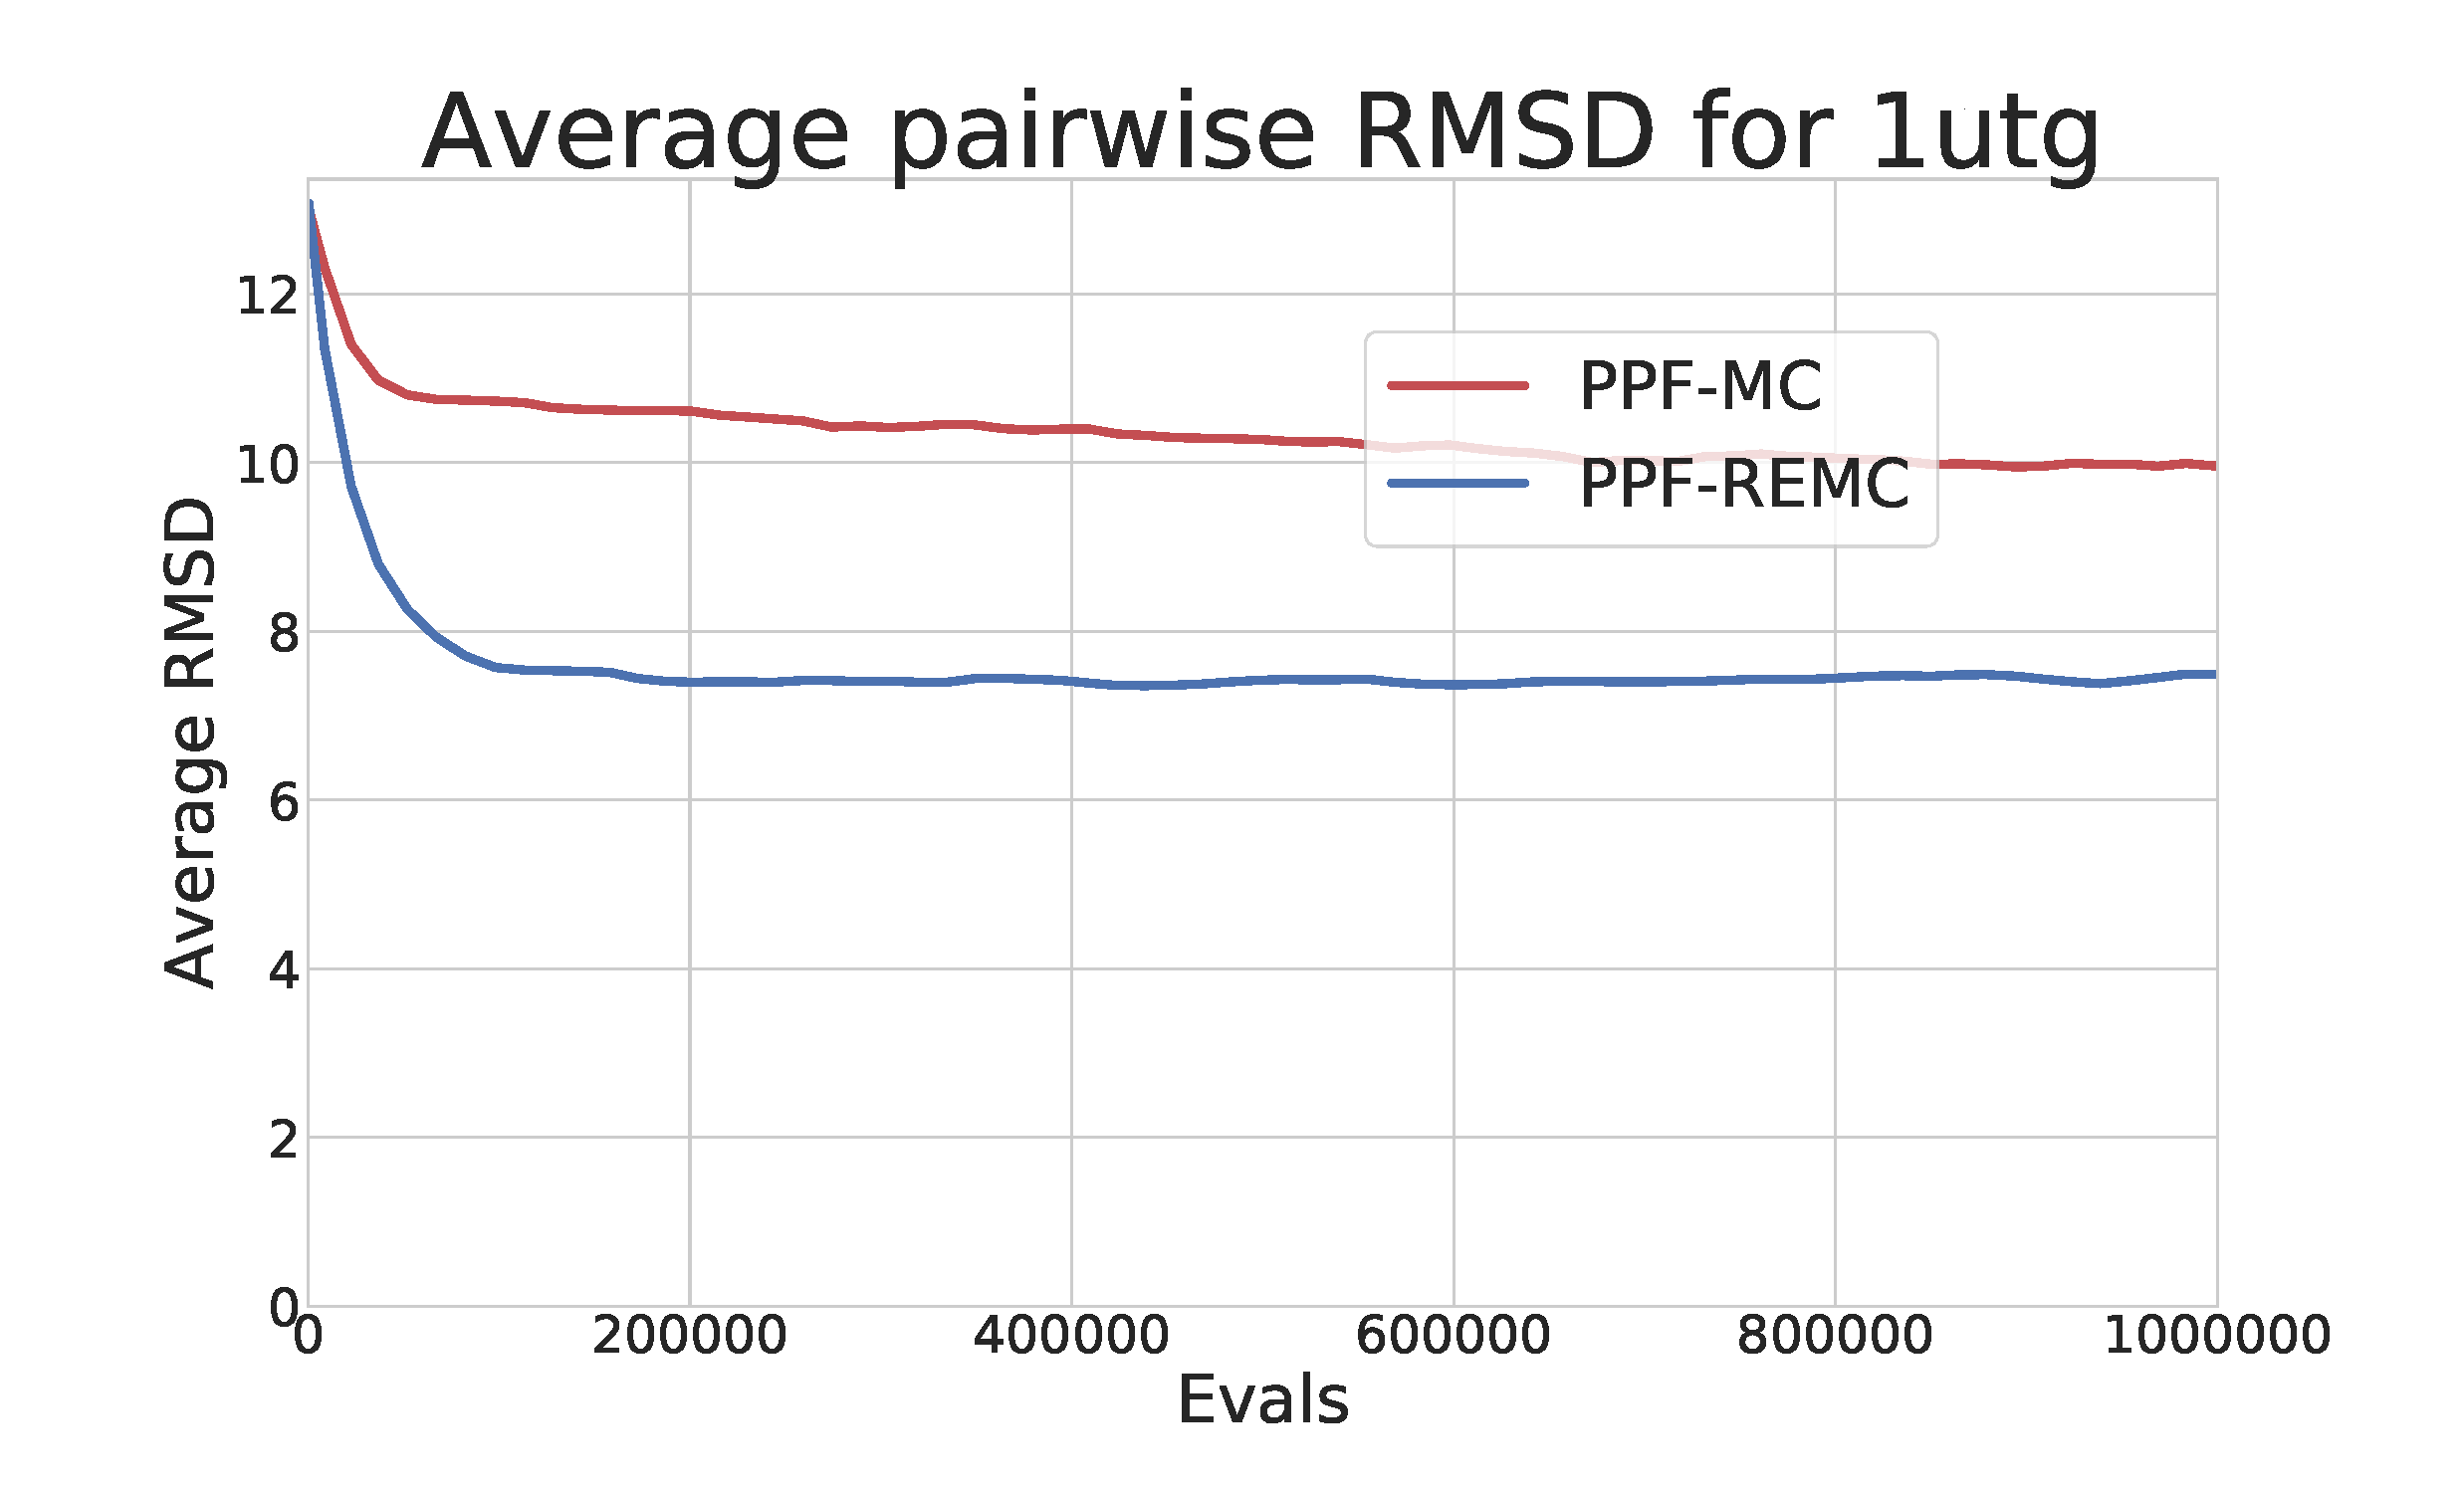
\includegraphics[width=1\linewidth]{Figuras/plots/rmsd_convergence/avg_rmsd_1utg.pdf}
    \caption{1utg}
    \label{fig:1utg-rmsd-convergence}
  \end{subfigure}
  \caption{The average pairwise RMSD for proteins 1rop and 1utg.
  The X Axis represents the function evaluations and
  the Y Axis indicates the value of the \texttt{score3} energy function being
  optimized.}
  \label{fig:rmsd-convergence-1rop-1utg}
\end{figure}

The genetopic convergence of the methods is presented in
Figure~\ref{fig:rmsd-convergence-1rop-1utg}, where the average pairwise RMSD of
the population is measured. Two proteins were selected as representatives.
Both proteins, 1rop and 1utg, have the same overall behavior as the other 8.
In both Figures~\ref{fig:1rop-rmsd-convergence}
and~\ref{fig:1utg-rmsd-convergence} ppf-remc has a lower diversity. For 9 of
the then proteins this distance is around 2 or less. Both methods sharply
decrease the diversity during the first few thousands function evaluations.
After that, it stays relatively stable. For ppf-mc, in some proteins, such as
1utg, the diversity slowly decreases. Since there is no exchange of information
between trajectories in this method, this indicates that the whole population
is slowly converging to the same direction. The sharp decrease in diversity for
ppf-remc is explained by its Replica Exchange mechanism, where one trajectory
can be compied to another, replacing it.

The protein where rppc-remc has the worst performance was 1rop, where it was
statistically worst than the other methods analysed. Comparing the average
diversity of both ppf derived methods, it is possible to see that there is a
gap of about $6$\AA, where the other proteins had a gap of $2$\AA  or less.
Since the population feeds the repacking stage with information, a low diversity
for such a big protein, might have lead to too many conformations being to close.
This, in turn generated clusters that are too close together.

With this analysis, is possible to detect that ppf-mc has better
convergence for the best individual than ppf-remc. However, when considering
the average energy of the population, ppf-remc has the best results.
Nevertheless, ppf-mc would be an interesting candidate for expanding the
budget of function evaluations available, since it keeps improving for a
longer period of time than ppf-remc and contains a bigger overall diversity in
the population.

\section{Monte Carlo vs Replica Exchange Monte Carlo}
\label{sec:methods-duel}
% Compare ppf-mc and ppf-remc

In this Section the two proposed methods are compared against each other, with
the goal of assessing if there is a method with a better performance. If that is
the case, then determing which one. For this, an initial visual inspection
using boxplots is first realized. Figures~\ref{fig:duel-boxplot-rmsd}
and~\ref{fig:duel-boxplot-energy} presents a direct comparison of the two
proposed methods. By inspecting the RMSD, in Figure~\ref{fig:duel-boxplot-rmsd},
it is possible to see that the two proposed methods closely match each other for
most of the proteins. For 1rop, was noticed in previous analysis, ppf-remc was
outmatched for all other methods being analysed. In fact, as confirmed by
Kruskal–Wallis (data not shown), 1rop is the only protein where there was
a statistical significance between the two proposed method.

\begin{figure}
  \centering
  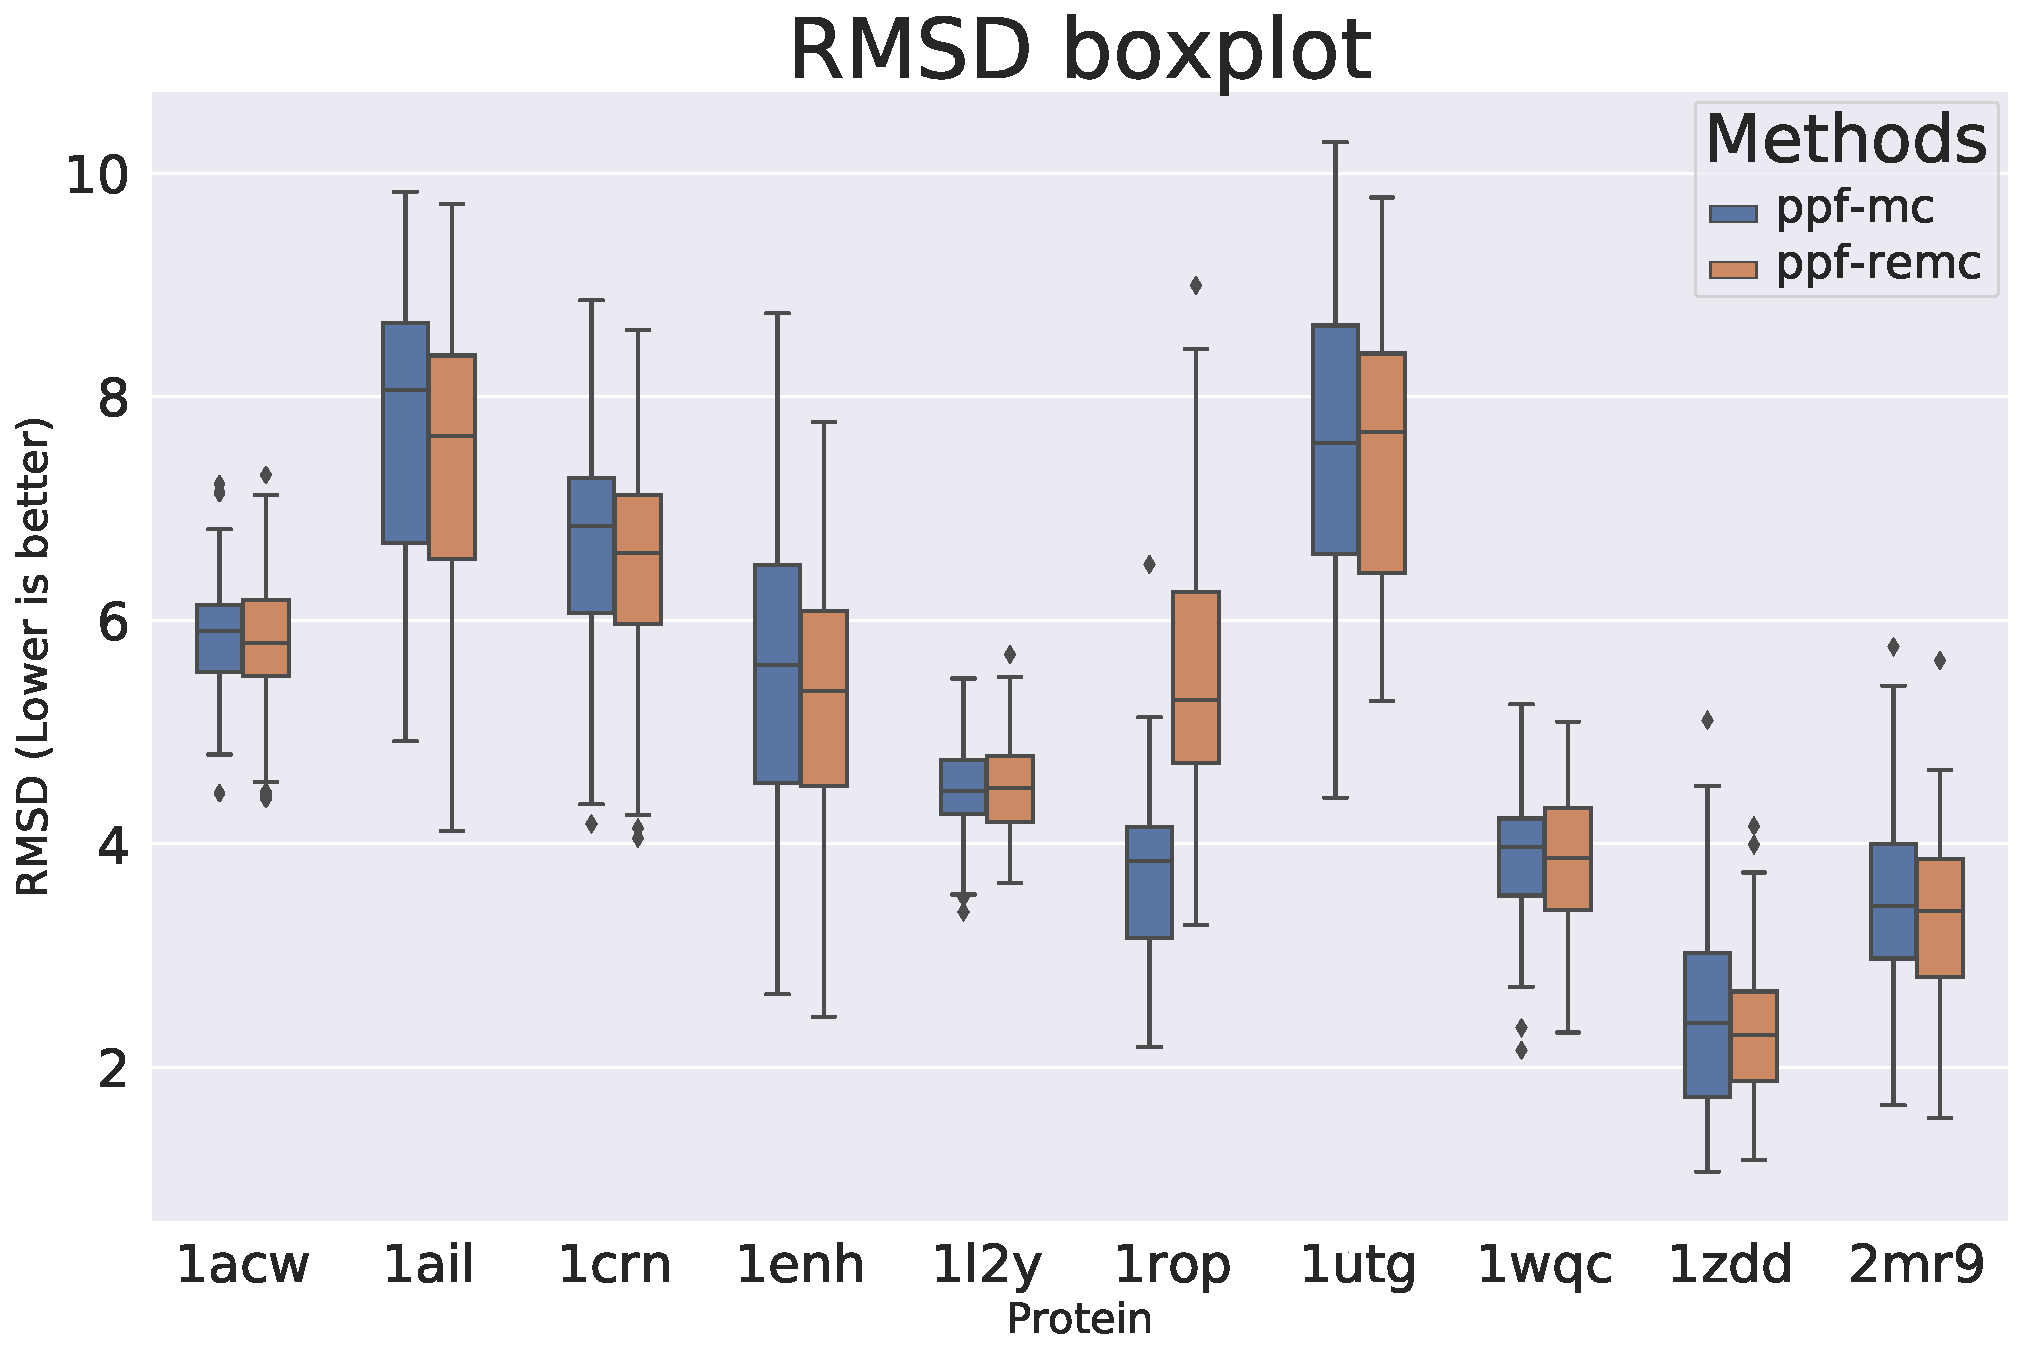
\includegraphics[width=1\textwidth]{Figuras/boxplots/duel_boxplot_best_by_rmsd_rmsd_after.pdf}
  \caption{RMSD comparison of PPF-MC and PPF-REMC.}
  \label{fig:duel-boxplot-rmsd}
\end{figure}

By analysing the Energy data, as displayed in
Figure~\ref{fig:duel-boxplot-energy}, it is possible to see that the performance
of the two proposed methods varied more than when RMSD was analysed. For protein
1rop, as expected, there is a clear difference in performance. However, for
several other proteins ppf-mc appears to have consistently reached lower
energies. In fact, by applying the Mann-Whitney test, ppf-mc outperformed
ppf-remc for proteins 1acw, 1ail, 1enh, 1rop and 2mr9.

\begin{figure}
  \centering
  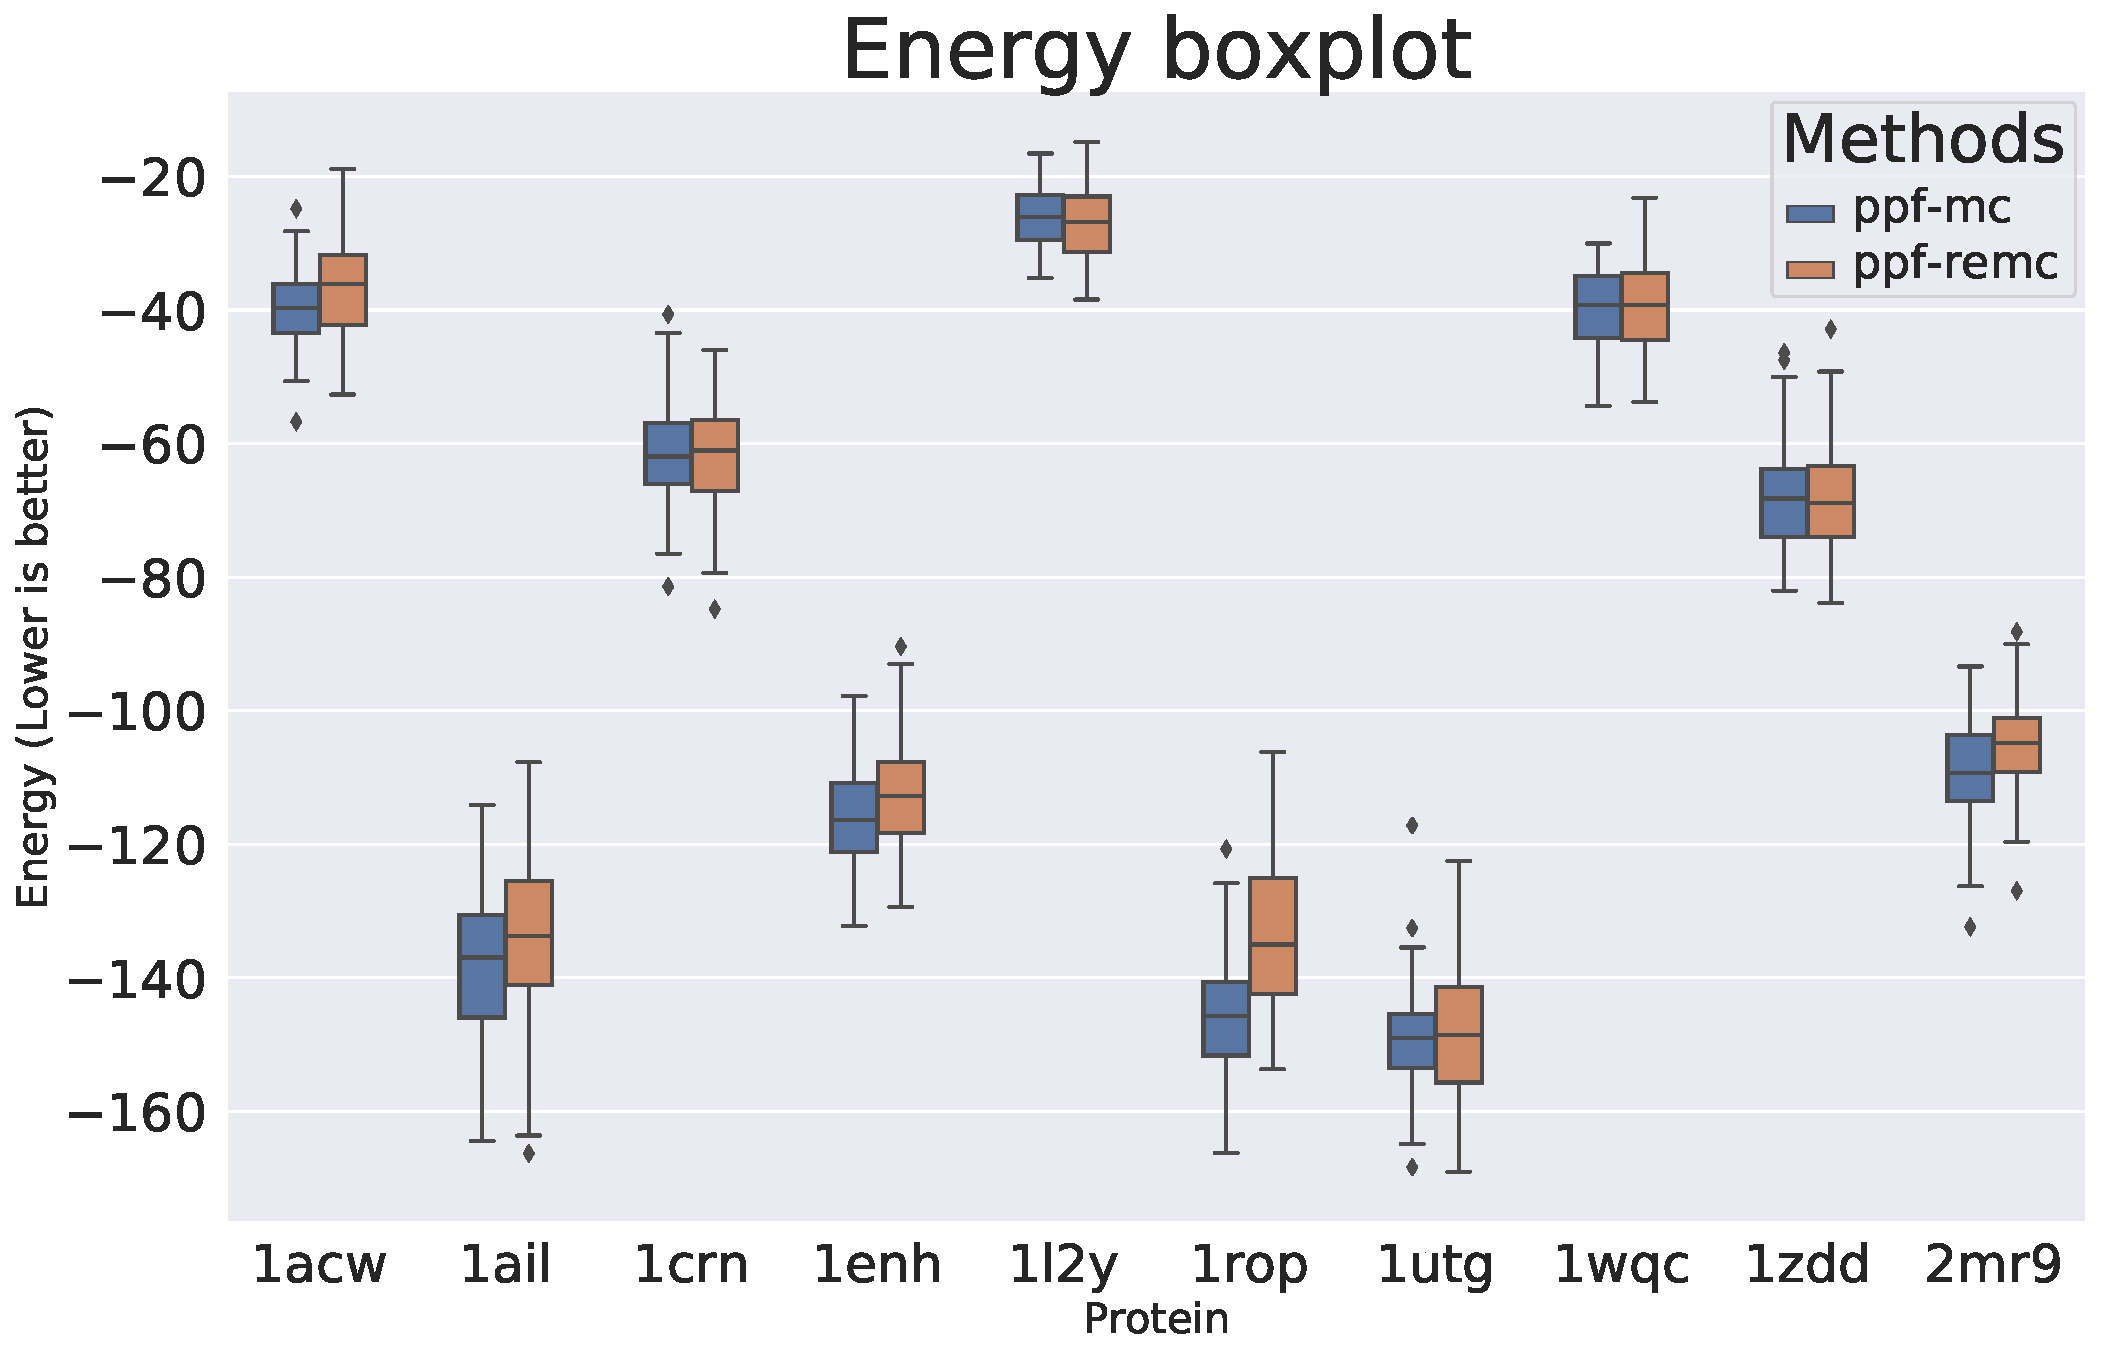
\includegraphics[width=1\textwidth]{Figuras/boxplots/duel_boxplot_best_by_energy_scorefxn}
  \caption{Energy comparison of PPF-MC and PPF-REMC.}
  \label{fig:duel-boxplot-energy}
\end{figure}

Interestingly, while ppf-mc outperformed ppf-remc for 1 protein considering
the rmsd and on 5 proteins, it also had the best conformation prediction
prediction in 5 of proteins too (data shown in Appendix~\ref{appendix:table-results}).
Furthermore, by combining this analysis with the one
from Section~\ref{sec:convergence-analysis}, where ppf-mc had a higher
diversity, a desirable property to match with clustering, it is safe to consider
ppf-mc as the better method of the two.

\section{Repacking Impact} \label{sec:repacking-impact}
% How much does the rmsd change before after
% If ranked by energy, does the ranking change before/after repacking

A major component of the proposed methods is the use of repacking. It allows for
the method to operate on a simplified model, with side chain represented as
centroids, that has a more smooth energy landscape and is fast to evaluate. On
the other hand, this model has reduced biological plausibility. As such,
repacking allows for this centroid model to be converted to a full atomic
representation of the protein. As such, investigating the impact that repacking
has is crucial in order to understand the performance of the proposed methods.
In order to understand it, two analysis must be made, one of the RMSD, which is
straight forward. The other, for the energy, is more complex. The energies before
and after the repacking are essentially different units of measure. Therefore, a
more careful analysis is required.

\begin{table}
  \centering
  \begin{tabular}{r|r|c||r|c||r|c}
            & \multicolumn{2}{c}{classic-abinitio} & \multicolumn{2}{||c}{ppf-mc} & \multicolumn{2}{||c}{ppf-remc} \\ \hline
    protein & mean      & stddev   & mean      & stddev   & mean      & stddev   \\ \hline \hline
    1acw    & $-0.1656$ & $0.3372$ & $0.2616$  & $0.4944$ & $0.2589$  & $0.5765$ \\ \hline
    1ail    & $-0.1113$ & $0.4629$ & $0.2470$  & $0.7731$ & $0.2379$  & $0.7278$ \\ \hline
    1crn    & $-0.0620$ & $0.4203$ & $-0.0297$ & $0.5865$ & $-0.1128$ & $0.4368$ \\ \hline
    1enh    & $-0.0558$ & $0.4854$ & $-0.1277$ & $0.5577$ & $-0.1380$ & $0.6081$ \\ \hline
    1l2y    & $0.2505$  & $0.3773$ & $0.3856$  & $0.5036$ & $0.6653$  & $0.7176$ \\ \hline
    1rop    & $0.8336$  & $0.4484$ & $0.7814$  & $0.9170$ & $1.2214$  & $1.3530$ \\ \hline
    1utg    & $-0.3506$ & $0.4712$ & $0.1346$  & $0.5762$ & $0.1793$  & $0.7202$ \\ \hline
    1wqc    & $-0.2543$ & $0.4381$ & $0.1729$  & $0.5624$ & $0.2160$  & $0.6377$ \\ \hline
    1zdd    & $0.2283$  & $0.4144$ & $0.7429$  & $0.6098$ & $0.7470$  & $0.9897$ \\ \hline
    2mr9    & $-0.2667$ & $0.6094$ & $0.2190$  & $0.5679$ & $0.1875$  & $0.6957$ \\ \hline
  \end{tabular}
  \caption{RMSD change caused by repacking}
  \label{tab:repack-impact-rmsd}
\end{table}

Table~\ref{tab:repack-impact-rmsd} presents the RMSD delta from before and after
the repacking. A negative delta value indicated that repacking increased the RMSD,
i.e. made it worse. Conversely, a positive value indicates that the RMSD decreased,
i.e. improved.
Since the proposed methods are mainly compared against rosetta,
it was included here as well. With this, it is possible to detect if repacking
gave unfair advantage to any of the three methods. A few patterns are detected
in the results. Firstly, both 1crn and 1enh had a increase of RMSD. While
relatively small, specially for rosetta, it is interesting that it happened for
the two proteins for all three methods. No other protein has this happen.
Another interesting point is that with the exception of 1l2y, 1rop and 1zdd,
rosetta had an increase of RMSD for all the remaining seven proteins. The
biggest mean difference was on 1utg, with a value of $-0.3506$. Comparing these
results with the medians from Table~\ref{fig:boxplot-rmsd} shows that the
impact of repacking for the RMSD has no impact in the statistical tests. Rosetta,
for 1utg, had a median above $10$, while the two proposed methods had a median
below $8$. Finally, the third noteworthy aspect of the results is that the only
mean above $1$ was on 1rop for ppf-remc, which had the worst performance
on that protein. This result could be explained due to the method having poor
optimization performance for this particular case. As such, repacking had more
room for improvement.

The energy impact of using repacking is more complex to conduct. As an
alternative of doing a direct delta of the values before and after, it is
possible to apply the same statistical analysis from
Section~\ref{sec:methods-analysis}. The results can then be compared
against Table~\ref{tab:mann-whitney-summary-rosetta-best-by-energy-scorefxn}.
If the repacking procedure had an unfair advantage to any of the methods
it will be detectable.

\begin{table}
  \centering
  \begin{tabular}{r|r|r|r}
  Protein & Wins & Loses & Draws \\ \hline \hline
   1acw &  2 &  0 &  0 \\ \hline
   1ail &  0 &  0 &  2 \\ \hline
   1crn &  1 &  1 &  0 \\ \hline
   1enh &  1 &  0 &  1 \\ \hline
   1l2y &  2 &  0 &  0 \\ \hline
   1rop &  2 &  0 &  0 \\ \hline
   1utg &  2 &  0 &  0 \\ \hline
   1wqc &  2 &  0 &  0 \\ \hline
   1zdd &  2 &  0 &  0 \\ \hline
   2mr9 &  2 &  0 &  0 \\ \hline
  \end{tabular}
  \caption{Summary of Mann-Whitney using score3, using the energy before repacking.
  The two proposed methods are compared agaisnt rosetta.}
  \label{tab:mann-whitney-summary-best-by-energy-score3}
\end{table}

The same sequence of statistical tests from
Section~\ref{sec:methods-analysis} were applied again, but now, only
considering the energy from before repacking, as scored by~\texttt{score3}.
In order to keep the analysis short, yet complete, only a summary of the
results is provided, presented in
Table~\ref{tab:mann-whitney-summary-best-by-energy-score3}.
This table can directly be compared against
Table~\ref{tab:mann-whitney-summary-rosetta-best-by-energy-scorefxn}.
It is worth noting that the results from Kruskal–Wallis (not shown) returned that there is
statistical difference for all the proteins, therefore, all proteins are
considered this time.

With the energy data from after the repacking, there were $2$ proteins,
2mr9 and 1utg, where the
two proposed methods outperformed rosetta. Using the data from before, there are
$7$ proteins (1acw, 1l2y, 1rop, 1utg, 1wqc, 1zdd and 2mr9).
A clear indicator that repacking had a considerable impact in the
energy of the final conformations. Furthermore, with \texttt{scorefxn} there
were two times were rosetta outperformed one of the proposed methods, with
\texttt{score3} there is only one. The number of draws between rosetta and the
proposed methods was also reduced. With \texttt{scorefxn} there were $12$
occurrences, while for \texttt{score3} here are $3$.

With these results, it is clear that repacking had a significant impact in the
energy of the final predicted conformations. By applying repacking, which is
essentially another optimizer, the results of the proposed methods and rosetta
reached close energy distributions several times. Nevertheless, even with
repacking the proposed methods were able to outperform rosetta in multiple
occasions. With this, it can be concluded two main points. Firstly, using
repacking did not benefit only the proposed methods. Secondly, repacking
appears to impact more the energy than RMSD.

\section{Processing time and functions evaluations} \label{sec:time-and-evals}

In Table~\ref{tab:processing-times} the processing times for the two proposed
methods are displayed. The first column shows the protein name, the second and
third column show the data for each of the methods. Each sub-column for the
methods contains the mean time and its standard deviation, measured in seconds.
The total processing time of the method does not include the preprocessing
steps, i.e. secondary structure prediction, the fragment picker, etc. The total
time considered is the sum of several steps of the algorithm. The time starts
counting for the main optimization phase when the initial population is
generated and it stops when the defined 1 million function evaluations is
spent. Then, the post processing phase starts, which is divided into three
sub steps. The first is the clustering, which overall averages less than a
second by itself. The second step is running Hooke-Jeeves for all the
conformations nearest to the cluster centroids. The final step is applying
repacking to the resulting conformations from Hooke-Jeeves. The final
processing time is the sum of all these steps.

\begin{table}
  \centering
  \begin{tabular}{r|c|c||c|c}
            & \multicolumn{2}{c}{ppf-mc} & \multicolumn{2}{||c}{ppf-remc} \\ \hline
    protein & mean & stddev & mean & stddev \\ \hline \hline
    1acw & $ 381.8566$ & $ 76.8664$ & $ 397.3399$ & $ 39.2449$ \\ \hline
    1ail & $1141.1461$ & $142.2935$ & $1127.3899$ & $139.9729$ \\ \hline
    1crn & $ 721.0492$ & $118.6126$ & $ 696.0591$ & $ 78.4302$ \\ \hline
    1enh & $ 763.7677$ & $ 86.2599$ & $ 783.4028$ & $ 95.5297$ \\ \hline
    1l2y & $ 252.8980$ & $ 19.1262$ & $ 252.7463$ & $ 18.8516$ \\ \hline
    1rop & $ 963.2695$ & $124.7610$ & $ 940.5557$ & $203.5212$ \\ \hline
    1utg & $1010.0412$ & $142.8927$ & $1018.6922$ & $193.5863$ \\ \hline
    1wqc & $ 341.4484$ & $ 35.1510$ & $ 346.3862$ & $ 36.6248$ \\ \hline
    1zdd & $ 462.3010$ & $127.2581$ & $ 483.3383$ & $ 50.8998$ \\ \hline
    2mr9 & $ 702.5817$ & $ 95.6492$ & $ 695.9580$ & $189.4521$ \\ \hline
  \end{tabular}
  \caption{Processing times, in seconds, for ppf-mc and ppf-remc}
  \label{tab:processing-times}
\end{table}

As expected, there is a direct correlation between the number of residues in a
given protein and the time required to predict its structure. The two smallest
proteins, 1l2y and 1wqc, had the faster processing times, while the bigger proteins,
1utg and 1ail, had the
highest times. The prediction times on average range from about 4 minutes up to
20 minutes per run.

For the majority of proteins, both methods had very close means. One interesting
difference noticed was the standard deviation for 1rop. For ppf-mc,
which had a relatively good prediction performance, on this protein it had
a standard deviation around $124$. The other method, ppf-remc, had a
standard deviation around $203$. There might be a correlation between the
poor performance of this method and the more spread out processing times.
For 1utg a similar situation happened, however, the performance of the two
methods was much closer.

Another performance analysis that can be made on top of the proposed methods
is the study of the spent function evaluations. The main optimization phase has
a fixed budged of 1 million function evaluations. The post-processing phase,
however, uses a separate budget, which is non fixed. The Hooke-Jeeves
search procedure is applied multiple times successively, until no improvement
is detected. In order to prevent a single run from running from too long or
using too many evaluations a strategy is employed. If a single call to
Hooke-Jeeves spends more than $5000$ evaluations, it is flagged for termination
at the next iteration. As such, each call spends around $5000$ to $6000$
evaluations. However, multiple calls can be made in succession.

\begin{table}
  \centering
  \begin{tabular}{r|c|c||c|c}
            & \multicolumn{2}{c}{ppf-mc} & \multicolumn{2}{||c}{ppf-remc} \\ \hline
    protein & mean         & stddev       & mean         & stddev \\ \hline \hline
    1acw    & $19894.6690$ & $9323.3251$  & $19818.5598$ & $8795.8194$  \\ \hline
    1ail    & $23215.9890$ & $12096.6411$ & $24927.3000$ & $11983.8881$ \\ \hline
    1crn    & $23704.9947$ & $11297.4331$ & $22657.6200$ & $10469.2788$ \\ \hline
    1enh    & $21141.6667$ & $11922.8046$ & $24419.4684$ & $13052.6594$ \\ \hline
    1l2y    & $16022.7659$ & $7145.3393$  & $15968.0817$ & $6859.0816$  \\ \hline
    1rop    & $21008.9153$ & $11595.2773$ & $23404.5686$ & $11476.0593$ \\ \hline
    1utg    & $23257.8303$ & $13708.3805$ & $26221.2802$ & $20265.7668$ \\ \hline
    1wqc    & $18342.0987$ & $8163.8972$  & $18962.6016$ & $8634.9350$  \\ \hline
    1zdd    & $21848.3618$ & $10229.3850$ & $21914.6842$ & $9503.5863$  \\ \hline
    2mr9    & $22260.8176$ & $11415.6200$ & $24356.2630$ & $31478.7399$ \\ \hline
  \end{tabular}
  \caption{Function evaluations spent on Hooke-Jeeves, for ppf-mc and ppf-remc}
  \label{tab:spent-evals}
\end{table}

Table~\ref{tab:spent-evals} presents the mean spent function evaluations and
the respective standard deviations. For all ten proteins and the two methods,
the mean stays relatively close to $20000$. A manual inspection of the logs
reveals that no methods spent more than $100000$ evaluations, with two rare
exceptions. As can be seem for 1utg and 2mr9, the standard deviation is very
large. The root cause of this value is a single outlier in each of the runs
for these proteins. For 2mr9 there was a single call to Hooke-Jeeves which spent
$803278$ function evaluations. The same happened with 1utg, where a single call
spent $412117$ function evaluations. Nevertheless, by inspection the logs it
was found that all these function evaluations did not impact the energy nor the
RMSD. %In fact, it appears that the root cause of such a high amount of spent energy evaluations was spent due to numeric instability, which caused a fault in the convergence of the method.

\section{Comparison with Competing Methods}
\label{sec:competing-methods}
% Big table here

A comparison against methods in the literature is very difficult to conduct.
Most of the methods in the literature are relatively superficial in their
explanations of how a given algorithm was implemented and what testing
methodology was employed. Paper space seems to be a possible cause for this,
since articles that spans more pages are usually more detailed about the
implementation and methodology. As such, a comparison has to be based on the
data provided in the works, which in most cases is not enough for a proper
rigorous analysis to be conducted. Nevertheless, this work attempts to provide
a simple framework for comparing the proposed methods with works in the
literature. Several works were selected, where the model utilized was the
full atomic model with and ab initio method, and their proteins and the RMSD
of the best prediction was recorded. From these, the proteins which appeared in
more than four works were selected.

\begin{sidewaystable}
  \begin{tabular}{c|l|c|c|c|c|c|c|c|c|c|c} \hline \hline
    Year & Source                            & 1ROP  & 1CRN  & 1UTG  & 1ZDD & 1ENH  & 2MR9 & 1L2Y & 1ACW  & 1AIL  & 1WQC \\ \hline \hline
%
    2019 & sade-remc-final                   & 3.28  & 4.14  & 5.28  & 1.17 & 3.26  & 1.55 & 3.65 & 4.40  & 4.79  & 2.31 \\ \hline
    2019 & sade-mc-final                     & 2.18  & 4.35  & 4.41  & 1.07 & 2.74  & 1.66 & 3.39 & 4.45  & 4.92  & 2.15 \\ \hline
%
    2019 & Rosetta                           & 3.46  & 4.30  & 8.03  & 0.91 & 2.84  & 2.48 & 4.83 & 5.85  & 4.75  & 2.50 \\ \hline
%
    2019 & {\cite{silva2019self}}            & -     & 6.08  & -     & 1.16 & 3.23  & -    & -    & -     & 4.46  & -    \\ \hline
    2019 & {\cite{narloch2019knowledge}}     & 6.02  & 4.53  & 6.38  & 2.35 & 5.56  & 2.49 & -    & 1.67  & -     & -    \\ \hline
    2018 & {\cite{song2018adoption}}         & 2.21  & 5.16  & 5.68  & 1.84 & 5.81  & -    & -    & -     & -     & -    \\ \hline
    2018 & {\cite{borguesan2018genetic}}     & -     & -     & 4.29  & -    & -     & 2.39 & -    & 2.00  & -     & -    \\ \hline
    2018 & {\cite{silva2018multistage}}      & -     & 6.96  & -     & 2.62 & 5.70  & -    & -    & -     & 8.27  & -    \\ \hline
    2017 & {\cite{de2018three}}              & 1.80  & 3.80  & 3.30  & 1.90 & 2.10  & 2.60 & 1.00 & -     & -     & 2.50 \\ \hline
    2017 & {\cite{narloch2017protein}}       & -     & 15.44 & -     & 9.42 & 19.28 & -    & -    & -     & 16.88 & -    \\ \hline
    2017 & {\cite{gao2018incorporation}}     & 3.07  & 5.34  & -     & -    & -     & -    & -    & -     & -     & -    \\ \hline
    2016 & {\cite{borguesan2016improving}}   & -     & -     & -     & -    & -     & 9.25 & -    & 11.10 & -     & 2.98 \\ \hline
    2016 & {\cite{venske2016ademo}}          & 4.48  & 6.06  & -     & -    & -     & -    & -    & -     & -     & -    \\ \hline
    2015 & {\cite{borguesan2015apl}}         & -     & 19.30 & -     & 9.50 & 20.23 & -    & -    & -     & 24.65 & -    \\ \hline
    2015 & {\cite{shehu2015review}}          & 3.37  & 4.43  & 3.60  & -    & -     & -    & -    & -     & -     & -    \\ \hline
    2015 & {\cite{rocha2015multiobjective}}  & -     & 4.98  & -     & -    & 4.23  & -    & 3.53 & -     & -     & 2.29 \\ \hline
    2013 & {\cite{olson2013off}}             & -     & -     & -     & -    & -     & -    & -    & -     & 3.90  & -    \\ \hline
    2013 & {\cite{brasil2013multiobjective}} & -     & 5.36  & -     & -    & 6.32  & -    & 2.31 & -     & -     & 2.97 \\ \hline
    2013 & {\cite{dorn2013knowledge}}        & -     & -     & -     & -    & -     & -    & 4.12 & 9.90  & -     & -    \\ \hline
    2013 & {\cite{venske2013multiobjective}} & -     & -     & -     & 2.16 & -     & -    & -    & -     & -     & -    \\ \hline
    2009 & {\cite{mansour2009scatter}}       & 17.25 & -     & 20.63 & -    & -     & -    & -    & -     & -     & -    \\ \hline
    2008 & {\cite{kehyayan2008evolutionary}} & 17.25 & -     & -     & -    & -     & -    & -    & -     & -     & -    \\ \hline
    2008 & {\cite{judy2009multi}}            & 3.48  & -     & 4.43  & 2.15 & -     & -    & -    & -     & -     & -    \\ \hline
    2006 & {\cite{cutello2005multi}}         & 3.70  & -     & 4.60  & 2.27 & -     & -    & -    & -     & -     & -    \\ \hline
  \end{tabular}
  \caption{A comparison of the RMSD from the best prediction}
  \label{tab:literature-comparison}
\end{sidewaystable}


In Table~\ref{tab:literature-comparison}, the results obtained are presented. The first
column indicates the year of the publication presented in
decreasing order. The column \textbf{Source} presents the source of the data, which is one of the proposed methods, the results
from rosetta, or a work in the literature. The
remaining columns present several proteins, sorted by the frequency in which it
appears in the literature. The data in these columns is the best RMSD from the
method in the given work.

Given that more than 20 works are cited in this table, doing a detailed
analysis and description would be rather cumbersome. Instead, some keynotes are
provided. First, there appears to be a weak trend where the RMSD is slowly
decreasing. Albeit this trend has several counter examples.
For instance, the works of~\cite{cazacu2014steel} and~\cite{judy2009multi}
have competitive results even by today standards, even though they are more than
a decade old. Another major point, is that the results are getting extremely
competitive in the last years. The competition probably is not any bigger due to
the lack of common proteins between the works. It is not rare to find works
from the same author where a different set of proteins is utilized.

Even in face of the competitiveness of the problem, the proposed methods were
able to achieve the best RMSD in a couple of proteins. In many other proteins
the results were competitive with the state of the art. For the protein 1wqc
the best RMSD was achieved by ppf-mc. On 2mr9 the proposed methods
achieved the best and second best results. For 1rop and 1crn, the two most used
proteins in the literature, one of the proposed methods was able to achieve
the second best result. The same occurred for 1enh. Another point worth stating
is that some proteins might be way too easy for the current methods. Take 1zdd
for example, all but two methods, the works from \citeonline{narloch2017protein}
and \citeonline{borguesan2015apl}, had RMSD smaller than 2.62. Considering that
most proteins in PDB have a resolution ranging from 1 to 2\AA, trying to go
smaller than that is more a pursue of luck than science. As such, this protein
might only be useful to validating new methods, but not for measuring progress.

\section{GDT-TS and TM-Score metrics}
\label{sec:other-metrics}

This section provides an in depth analysis of the results obtained in this
work using the GDT-TS and the TM-Score metrics of the predicted proteins.
The conformations analysed are the ones selected using \texttt{best-by-rmsd} strategy.
The results can also be used by other works to compare against our own using
these metrics. Tables~\ref{tab:gdtts-data} and~\ref{tab:tmscore-data} present
for the ppf-remc and ppf-mc, their
GDT-TS and TM-Score values, respectively. Both tables follows the same format. The
first column presents the protein name. The results for both methods are
presented in separated columns. Each one of the
method's column is split into three sub-columns with the best result, the mean
and the standard deviation, respectively.

Both GDT-TS and TM-Score share the same property where values can be used as
thresholds for prediction quality. A value close to $0.2$ indicates the performance of
a random prediction, while the value of $0.5$ or above indicates a prediction that has
the same overall fold. Considering that, values of $0.5$ or above are marked
in boldface font.

\begin{table}
  \centering
  \begin{tabular}{r|c|c|c||c|c|c}
            & \multicolumn{3}{c}{ppf-mc} & \multicolumn{3}{||c}{ppf-remc} \\ \hline
    Protein & best          & mean          & stddev   & best          & mean          & stddev   \\ \hline \hline
    1acw    & $\bm{0.5172}$ & $0.4605$      & $0.0302$ & $\bm{0.5603}$ & $0.4648$      & $0.0359$ \\ \hline
    1ail    & $0.4932$      & $0.3794$      & $0.0473$ & $\bm{0.5856}$ & $0.3999$      & $0.0710$ \\ \hline
    1crn    & $\bm{0.5870}$ & $0.4343$      & $0.0560$ & $\bm{0.5815}$ & $0.4245$      & $0.0525$ \\ \hline
    1enh    & $0.4861$      & $0.4262$      & $0.0369$ & $0.4907$      & $0.4425$      & $0.0328$ \\ \hline
    1l2y    & $\bm{0.6625}$ & $\bm{0.5773}$ & $0.0439$ & $\bm{0.6625}$ & $\bm{0.5657}$ & $0.0344$ \\ \hline
    1rop    & $\bm{0.6825}$ & $\bm{0.5772}$ & $0.0517$ & $\bm{0.6151}$ & $0.4985$      & $0.0551$ \\ \hline
    1utg    & $\bm{0.5571}$ & $0.4346$      & $0.0631$ & $\bm{0.5607}$ & $0.4391$      & $0.0508$ \\ \hline
    1wqc    & $\bm{0.7885}$ & $\bm{0.6446}$ & $0.0451$ & $\bm{0.7500}$ & $\bm{0.6390}$ & $0.0493$ \\ \hline
    1zdd    & $0.4412$      & $0.4193$      & $0.0160$ & $0.4338$      & $0.4060$      & $0.0166$ \\ \hline
    2mr9    & $\bm{0.8807}$ & $\bm{0.6891}$ & $0.0720$ & $\bm{0.8750}$ & $\bm{0.6920}$ & $0.0618$ \\ \hline
  \end{tabular}
  \caption{GDT-TS for ppf-mc and ppf-remc}
  \label{tab:gdtts-data}
\end{table}

Analysing the GDT-TS values, comparing one method against the other, there are no
major differences between the two methods.
With the exception of 1rop, due a difference of $0.0025$, all
methods had the same results regarding valued above $0.5$. In fact, both methods
have very similar results for all proteins, with little difference. The protein
with the biggest difference was 1rop, where the means were $0.0787$ units apart
and the best value was $0.0674$ units apart. Interestingly, 1zdd, the protein
with the lowest RMSD has a GDT-TS of $0.41$ and $0.43$ for the two methods.
Meanwhile, 1wqc and 2mr9 had values above $0.75$ and $0.87$, respectively.
Meaning that the two metrics, namely GDT-TS and RMSD, don't always agree.

\begin{table}
  \centering
  \begin{tabular}{r|c|c|c||c|c|c}
            & \multicolumn{3}{c}{ppf-mc} & \multicolumn{3}{||c}{ppf-remc} \\ \hline
    Protein & best          & mean          & stddev   & best          & mean          & stddev   \\ \hline \hline
    1acw    & $0.2475$      & $0.1930$      & $0.0202$ & $0.2583$      & $0.1945$      & $0.0280$ \\ \hline
    1ail    & $0.4468$      & $0.3039$      & $0.0457$ & $\bm{0.5461}$ & $0.3336$      & $0.0697$ \\ \hline
    1crn    & $0.3986$      & $0.2762$      & $0.0462$ & $0.3987$      & $0.2669$      & $0.0468$ \\ \hline
    1enh    & $0.3489$      & $0.2628$      & $0.0272$ & $0.3397$      & $0.2725$      & $0.0315$ \\ \hline
    1l2y    & $0.2495$      & $0.1924$      & $0.0294$ & $0.2304$      & $0.1771$      & $0.0362$ \\ \hline
    1rop    & $\bm{0.6229}$ & $0.4588$      & $0.0646$ & $\bm{0.5006}$ & $0.3915$      & $0.0565$ \\ \hline
    1utg    & $0.4938$      & $0.3676$      & $0.0632$ & $\bm{0.5154}$ & $0.3756$      & $0.0506$ \\ \hline
    1wqc    & $0.3757$      & $0.2852$      & $0.0346$ & $0.3861$      & $0.2831$      & $0.0463$ \\ \hline
    1zdd    & $0.3178$      & $0.2797$      & $0.0276$ & $0.3104$      & $0.2628$      & $0.0202$ \\ \hline
    2mr9    & $\bm{0.7514}$ & $\bm{0.5117}$ & $0.0900$ & $\bm{0.7456}$ & $\bm{0.5186}$ & $0.0769$ \\ \hline
  \end{tabular}
  \caption{TM Score for ppf-mc and ppf-remc}
  \label{tab:tmscore-data}
\end{table}

Considering the TM-Score, there is a very low number of values above the
threshold of $0.5$. Again, both methods had similar values overall with very
little difference. Furthermore, not only RMSD and GDT-TS disagree on some cases,
such as for 1zdd, 1wqc and 2mr9, but
TM-Score can differ from the other two metrics in some cases as well. For
instance, on 1wqc the GDT-TS value was $0.75$ or higher, while the respective
TM-Scores were $0.31$ or lower. Also, TM-Score evaluated some methods as having
a performance worst than random search for 1acw and 1l2y. This contradicts the results
both from RMSD and GDT-TS.

One noteworthy aspect of GDT-TS and TM-Score is that they appear to be more
rigorous than RMSD. Take 1enh for example, it had the second best RMSD found
in the literature, yet, with GDT-TS, it did not make the cut of $0.5$. More so,
both 1enh and 1ail, two relatively big proteins, had their best RMSD more
than two units apart with ppf-mc. However, with the GDT-TS for the same
method, the two conformations are less than $0.01$ units apart. This is possible
due to RMSD being a metric with an unbounded upper limit, which scales
quadratically with the number of residues. GDT-TS on the other hand, has a
normalized value between $0$ and $1$, which allows the predictive performance
to be compared not only across different methods, but across proteins of different sizes.
Unfortunately, very few works in the literature use these metrics. This work,
with the goal of improving future comparisons of higher quality than the allowed
at the time of writing this work, shares these metrics. Complementary, the raw data is
provided in Appendix~\ref{appendix:gdtts-data} and~\ref{appendix:tmscore-data},
with the goal of allowing future methods to do a rigorous statistical analysis
using this one as reference.

\textcolor{red}{
Furthermore, considering that TM-Score had a tendency to underestimate the quality
of the predictions, it might not be the best for tracking performance in a
method under development. On the other hand, GDT-TS was able to identify both
good and bad predictions, making it a more suitable metric for such conditions.
}

\section{Visual Representation of the Predictions}
\label{sec:visual-analysis}

A final step in the analysis of the proposed methods is to do a visual
inspection. Considering that two methods were proposed, and that there are 10
proteins being analysed, comparing the 20 best predictions would be very
extensive. For this reason, ppf-mc was selected to be inspected, since
its predictions were overall more accurate.

\begin{figure}
  \begin{subfigure}{0.24\linewidth}
    \centering
    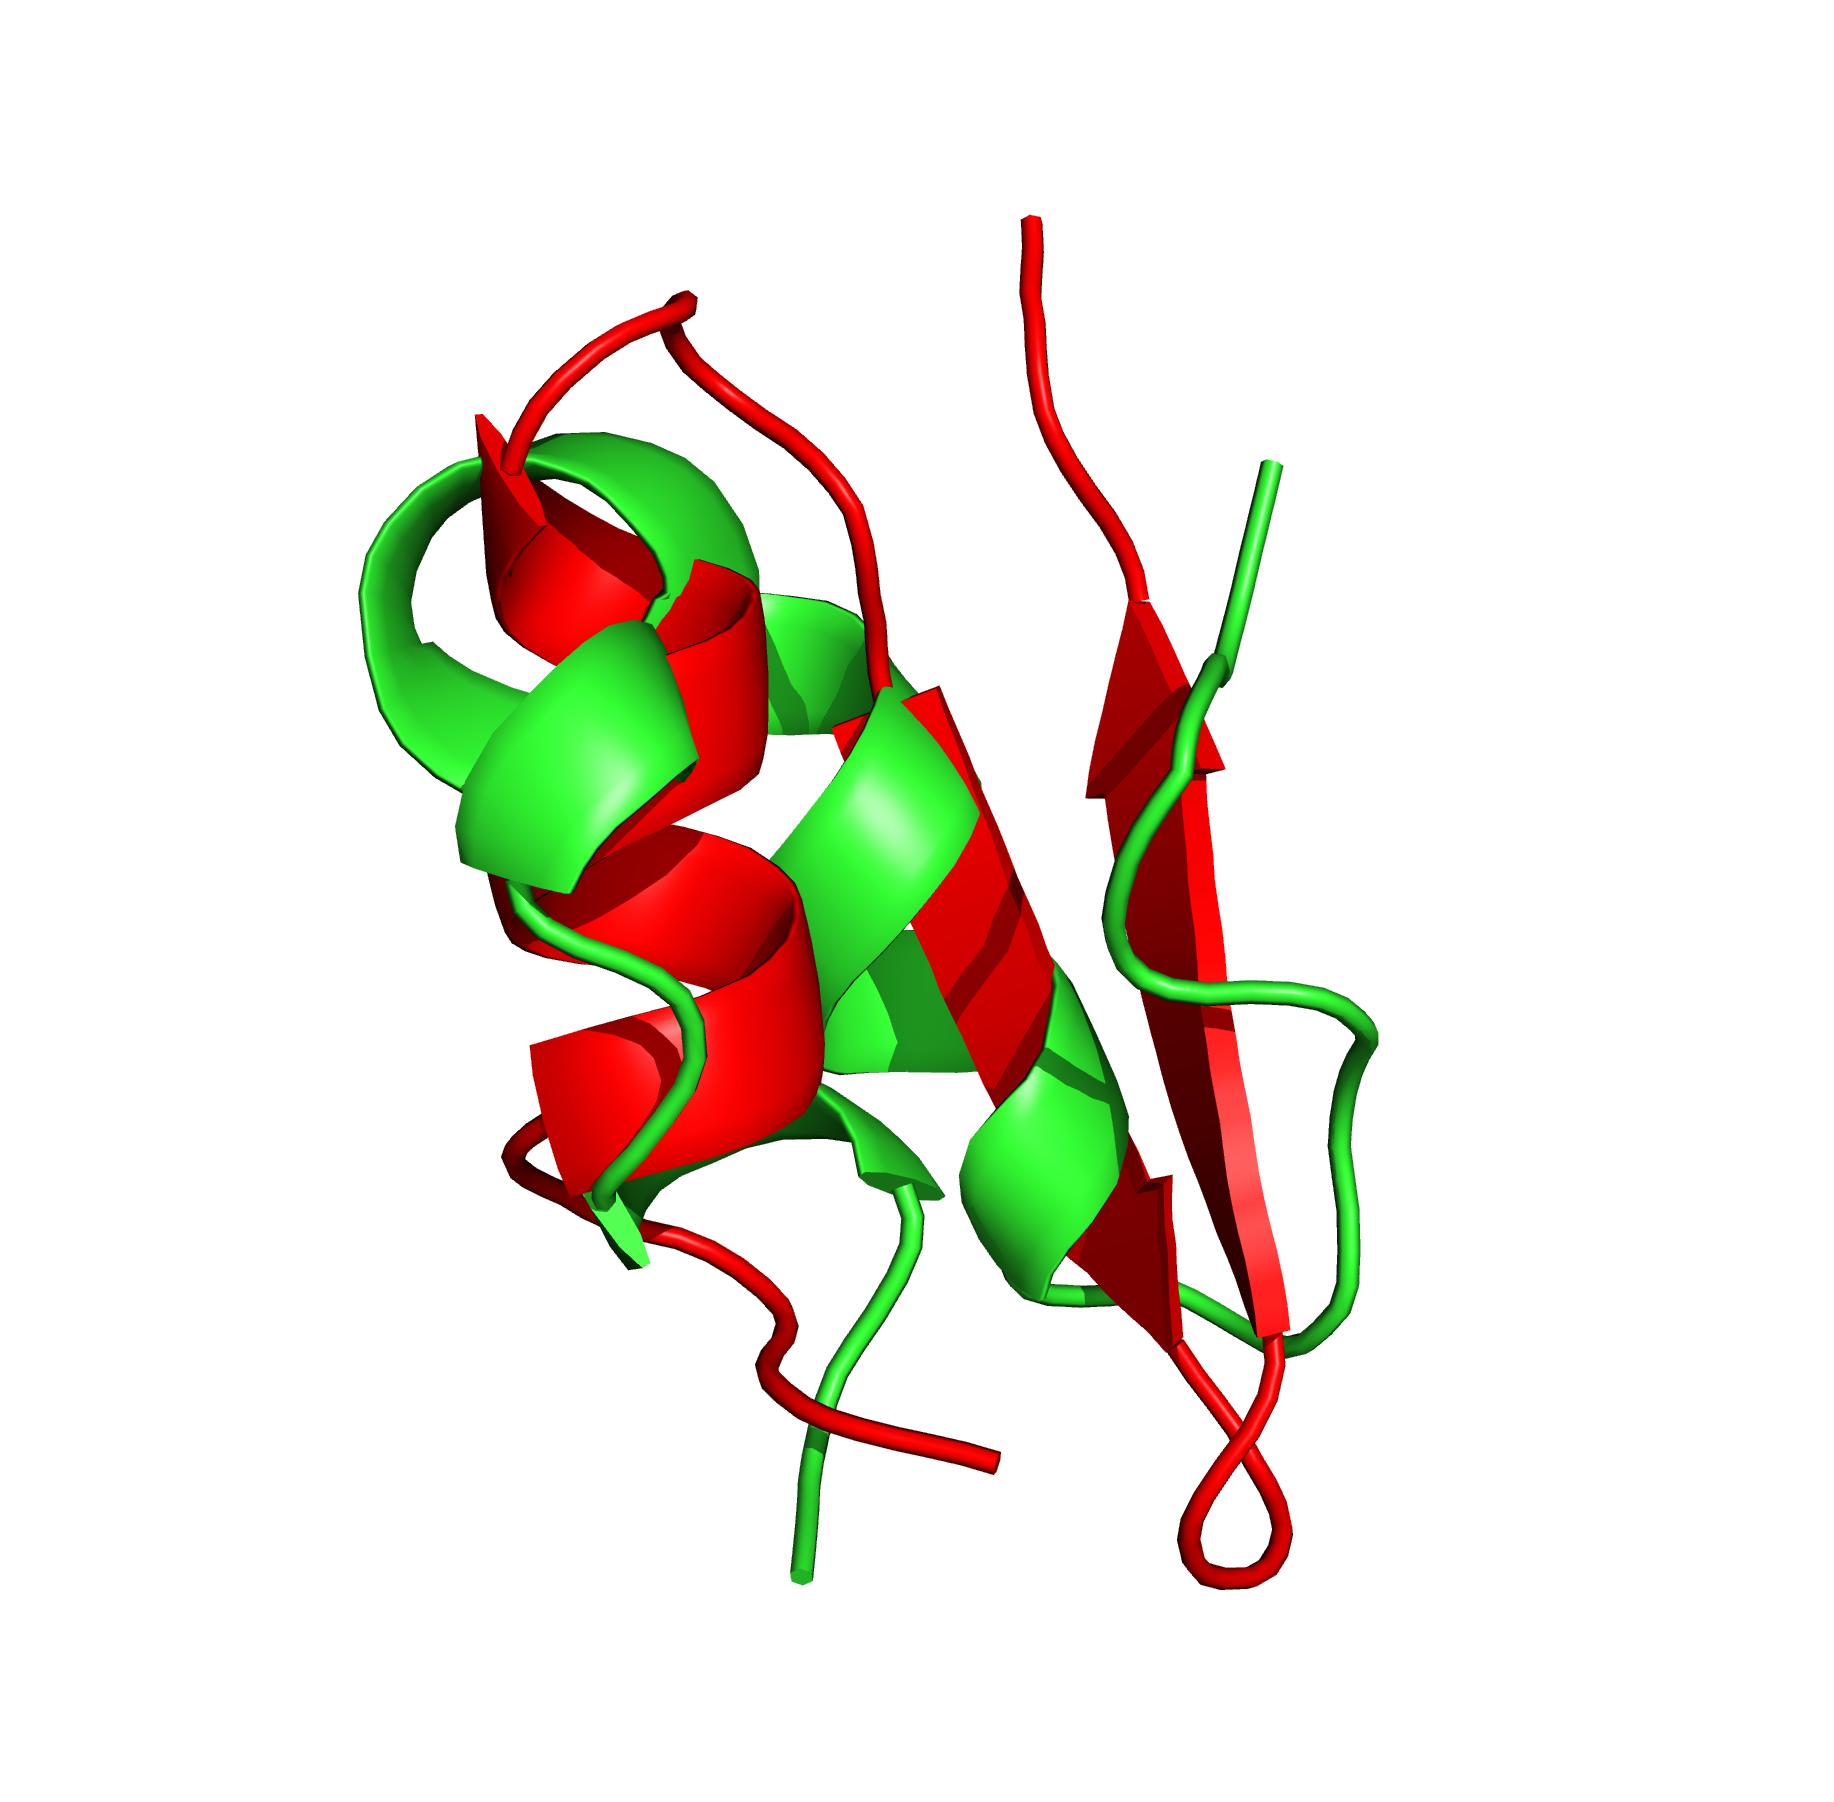
\includegraphics[width=0.9\linewidth]{Figuras/prots/1acw_render.png}
    \caption{1acw (4.45\AA)}
    \label{fig:1acw-conformation}
  \end{subfigure}
%
  \begin{subfigure}{0.24\linewidth}
    \centering
    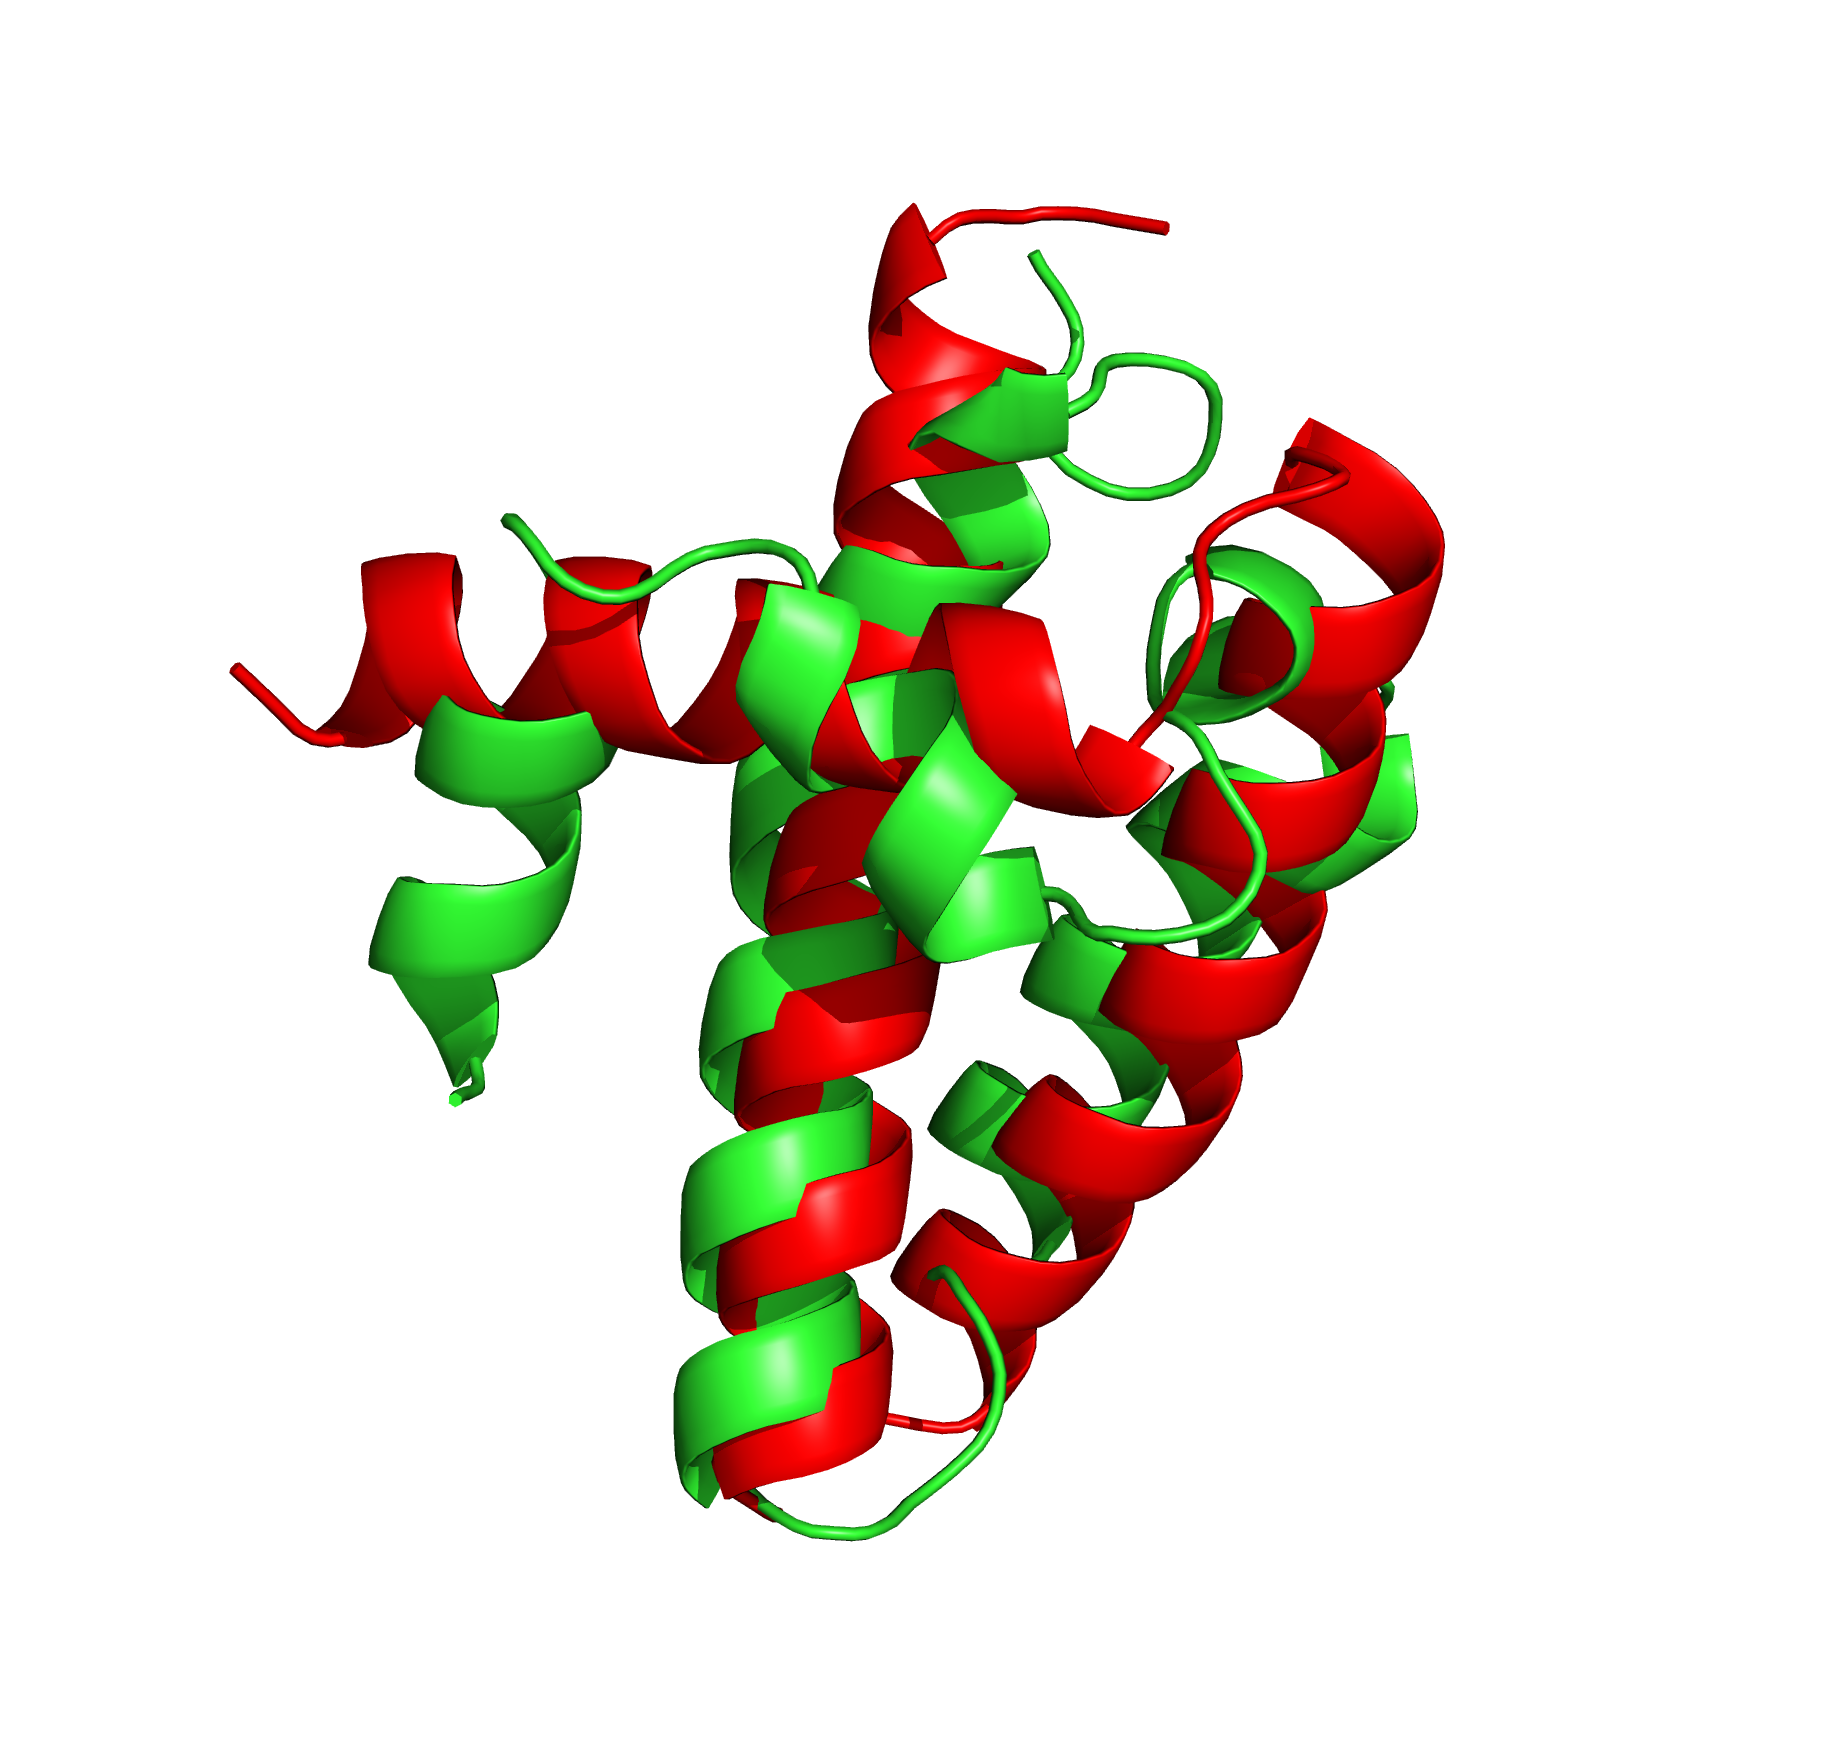
\includegraphics[width=0.9\linewidth]{Figuras/prots/1ail_render.png}
    \caption{1ail (4.26\AA)}
    \label{fig:1ail-conformation}
  \end{subfigure}
%
  \begin{subfigure}{0.24\linewidth}
    \centering
    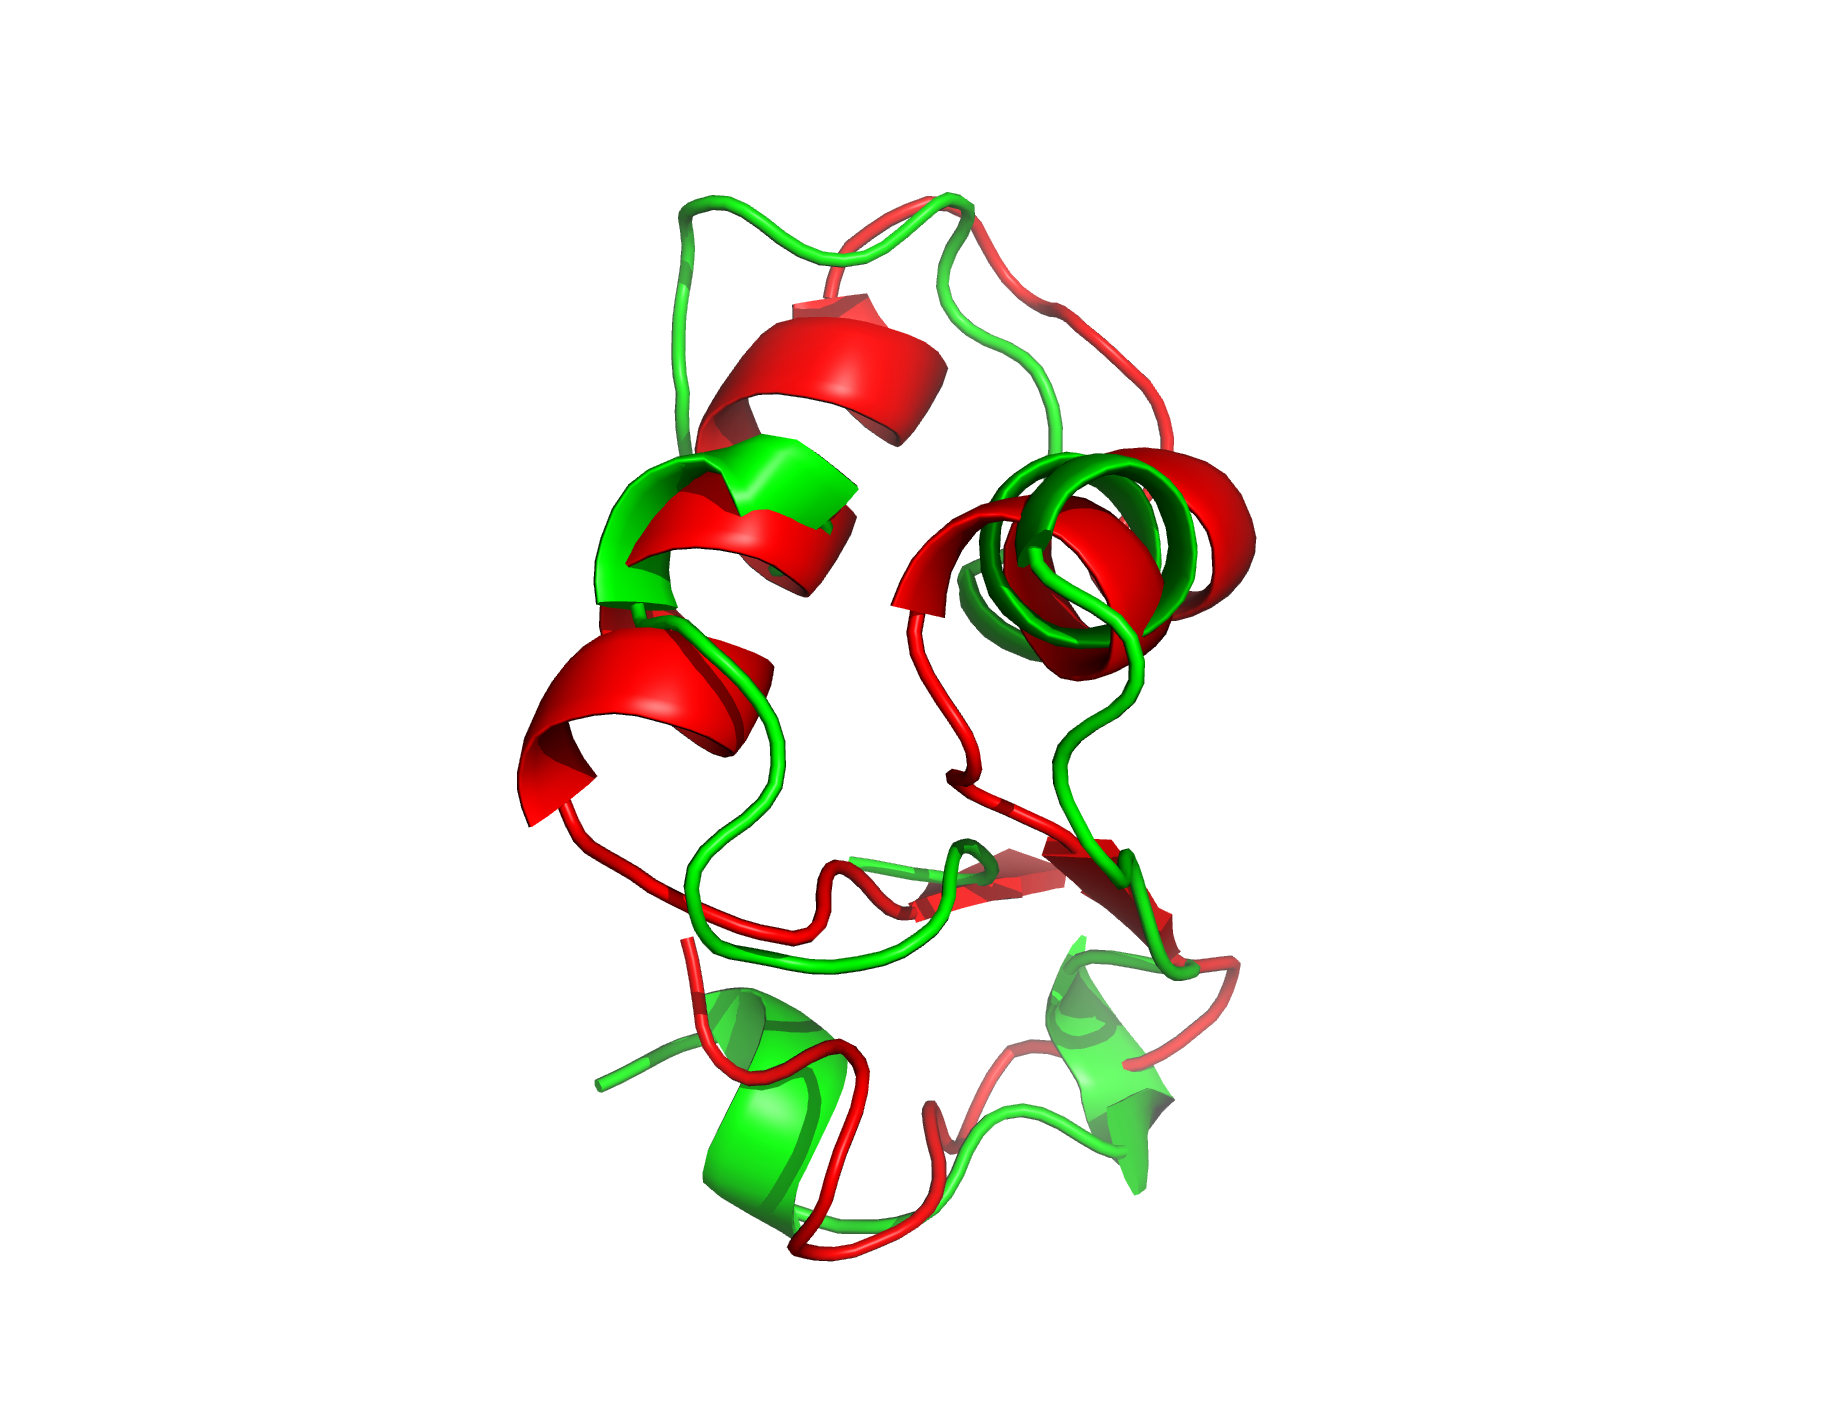
\includegraphics[width=0.9\linewidth]{Figuras/prots/1crn_render.png}
    \caption{1crn (4.18\AA)}
    \label{fig:1crn-conformation}
  \end{subfigure}
%
  \begin{subfigure}{0.24\linewidth}
    \centering
    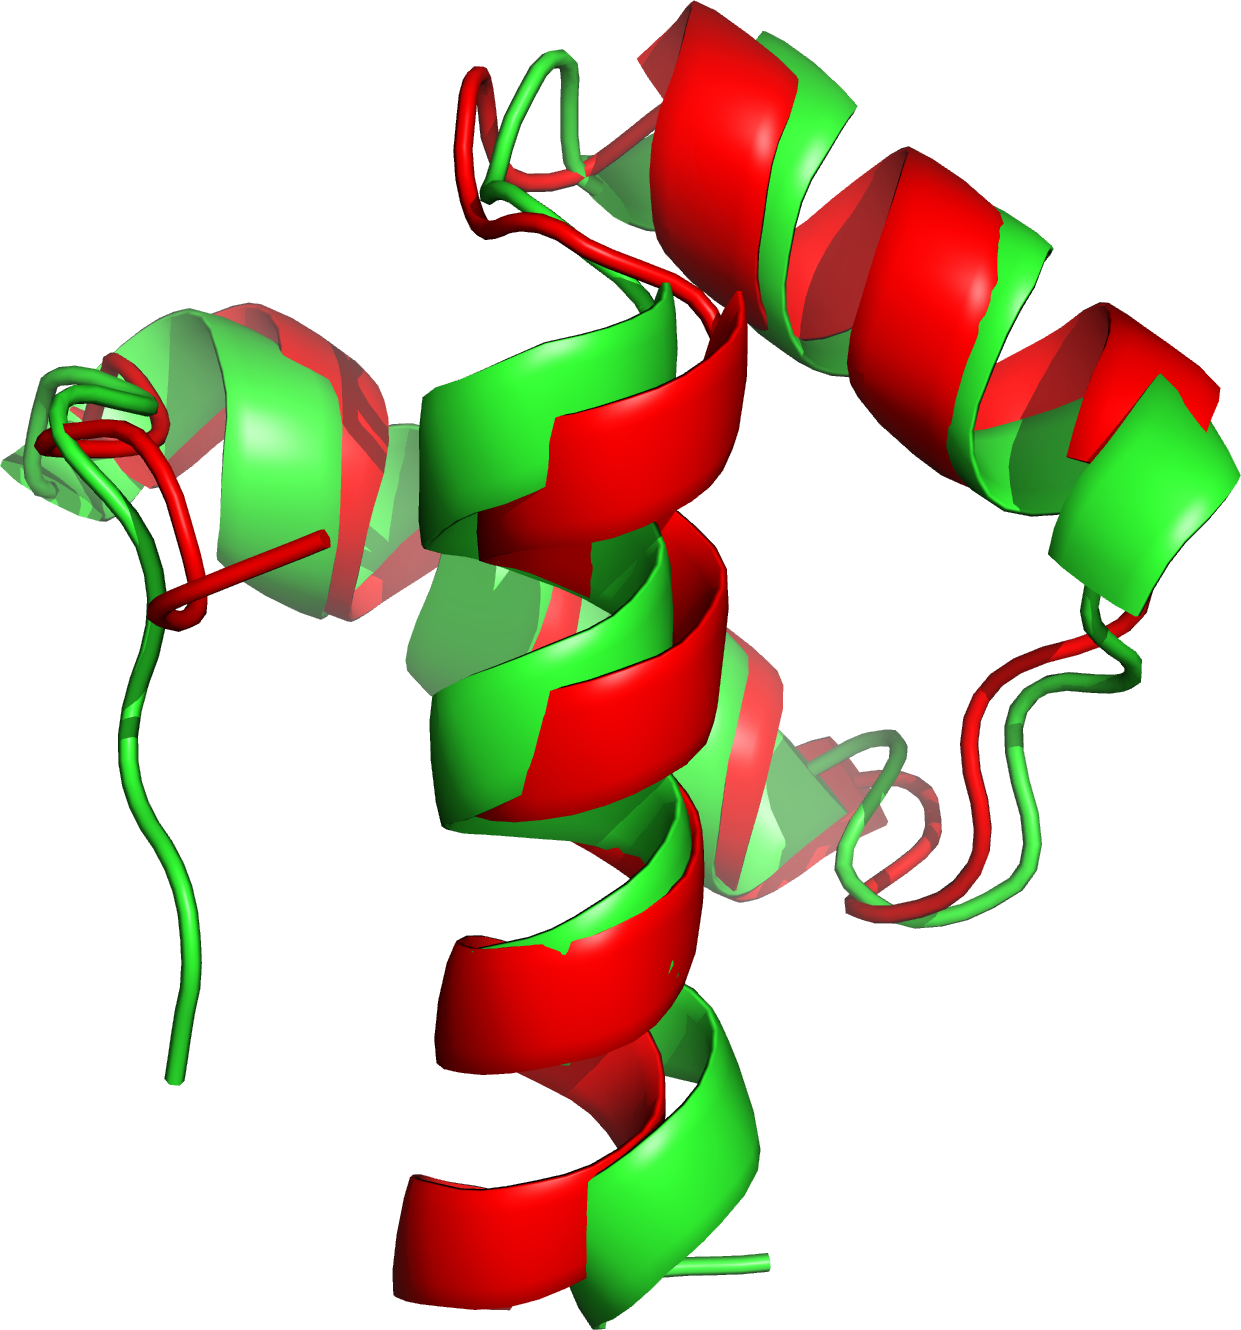
\includegraphics[width=0.9\linewidth]{Figuras/prots/1enh_render.png}
    \caption{1enh (2.65(\AA))}
    \label{fig:1enh-conformation}
  \end{subfigure}
% \end{figure}
% \begin{figure}
  \begin{subfigure}{0.32\linewidth}
    \centering
    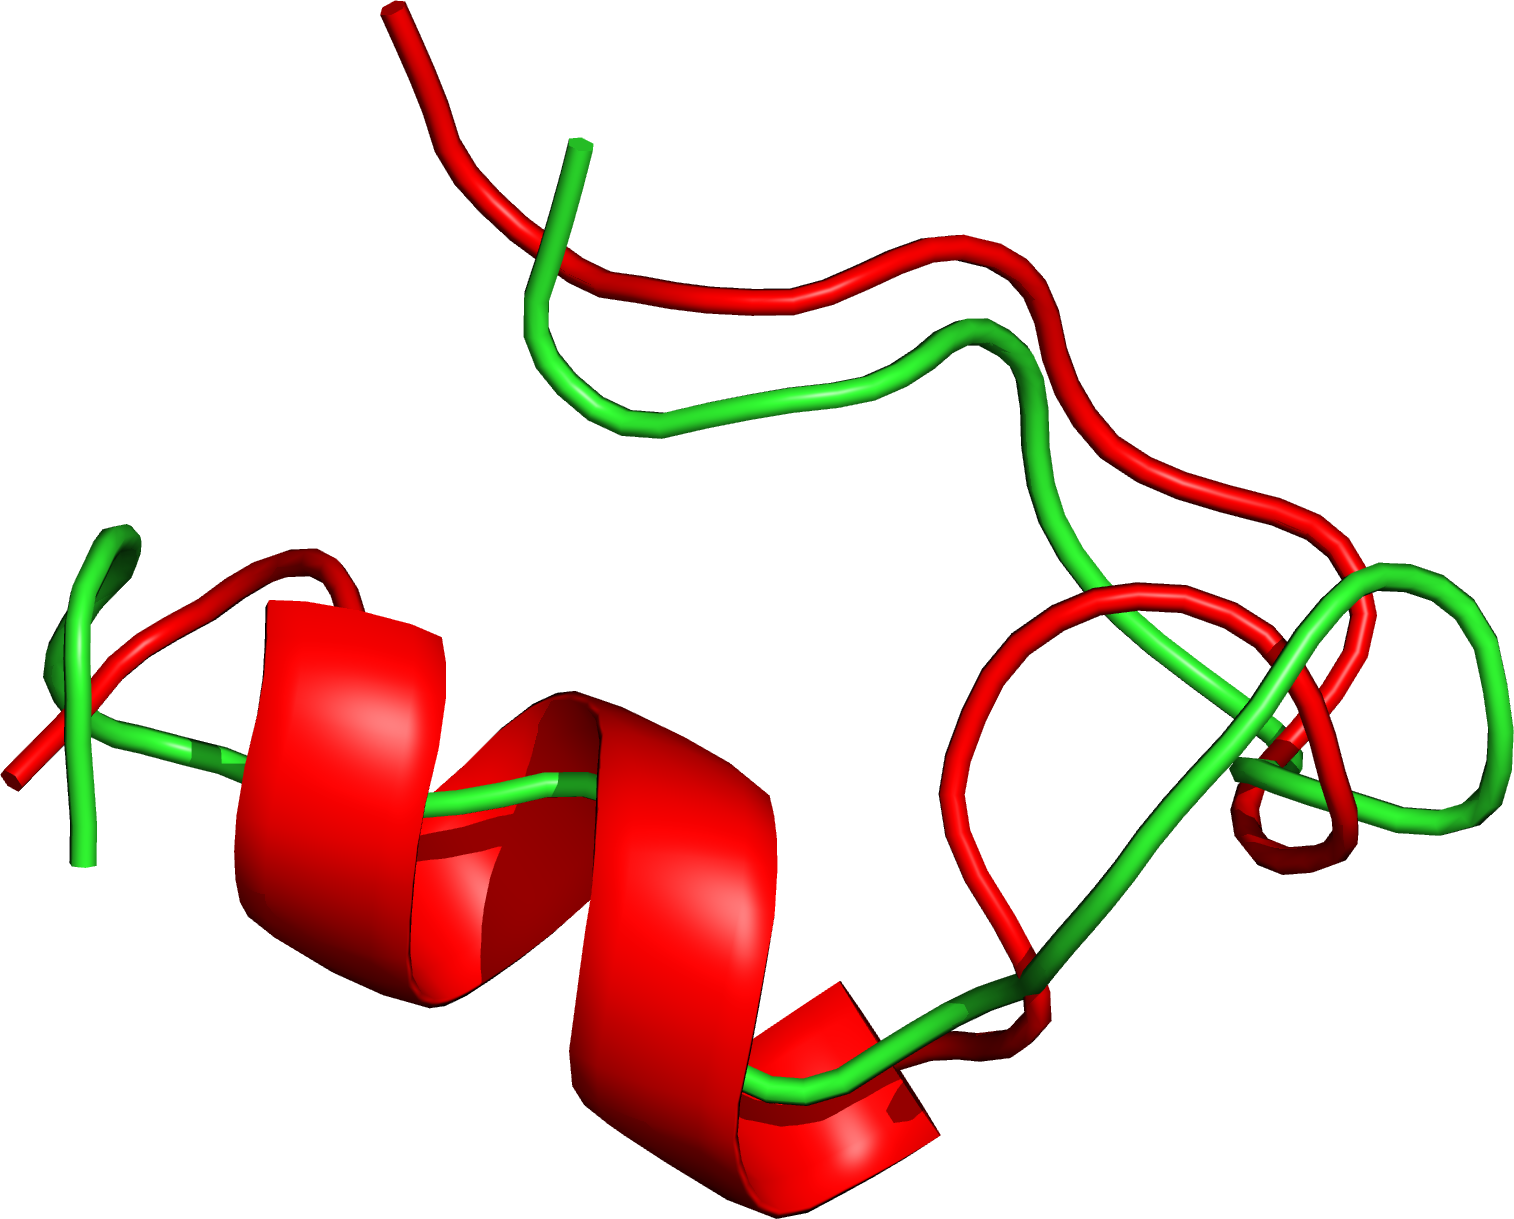
\includegraphics[width=0.9\linewidth]{Figuras/prots/1l2y_render.png}
    \caption{1l2y (3.39\AA)}
    \label{fig:1l2y-conformation}
  \end{subfigure}
%
  \begin{subfigure}{0.32\linewidth}
    \centering
    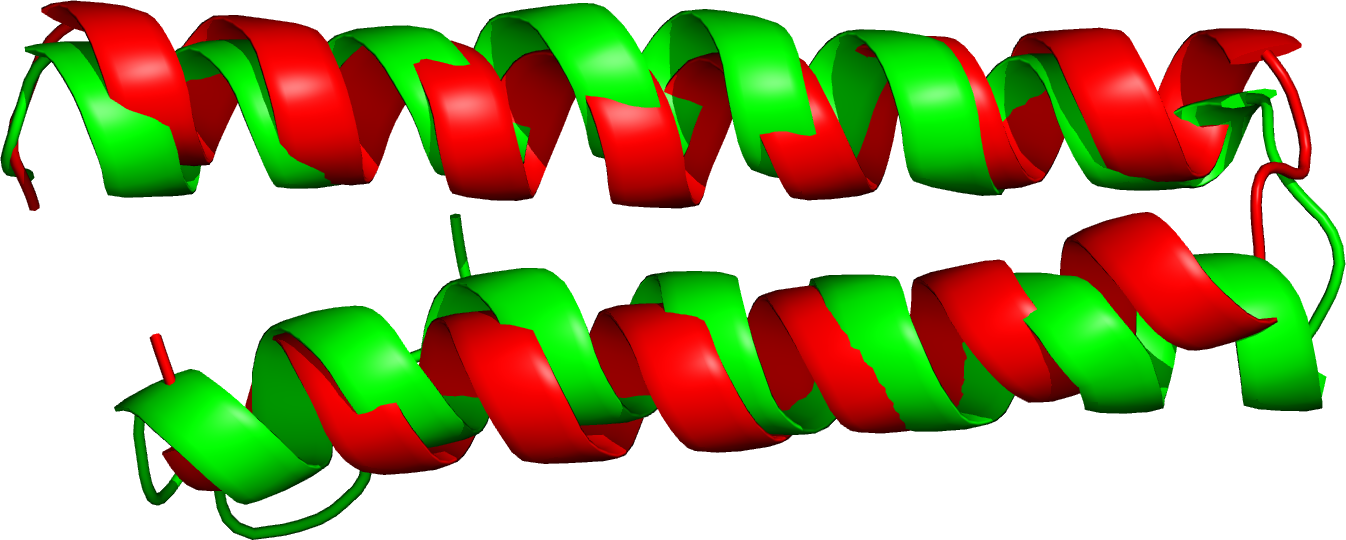
\includegraphics[width=0.9\linewidth]{Figuras/prots/1rop_render.png}
    \caption{1rop (2.18\AA)}
    \label{fig:1rop-conformation}
  \end{subfigure}
%
  \begin{subfigure}{0.32\linewidth}
    \centering
    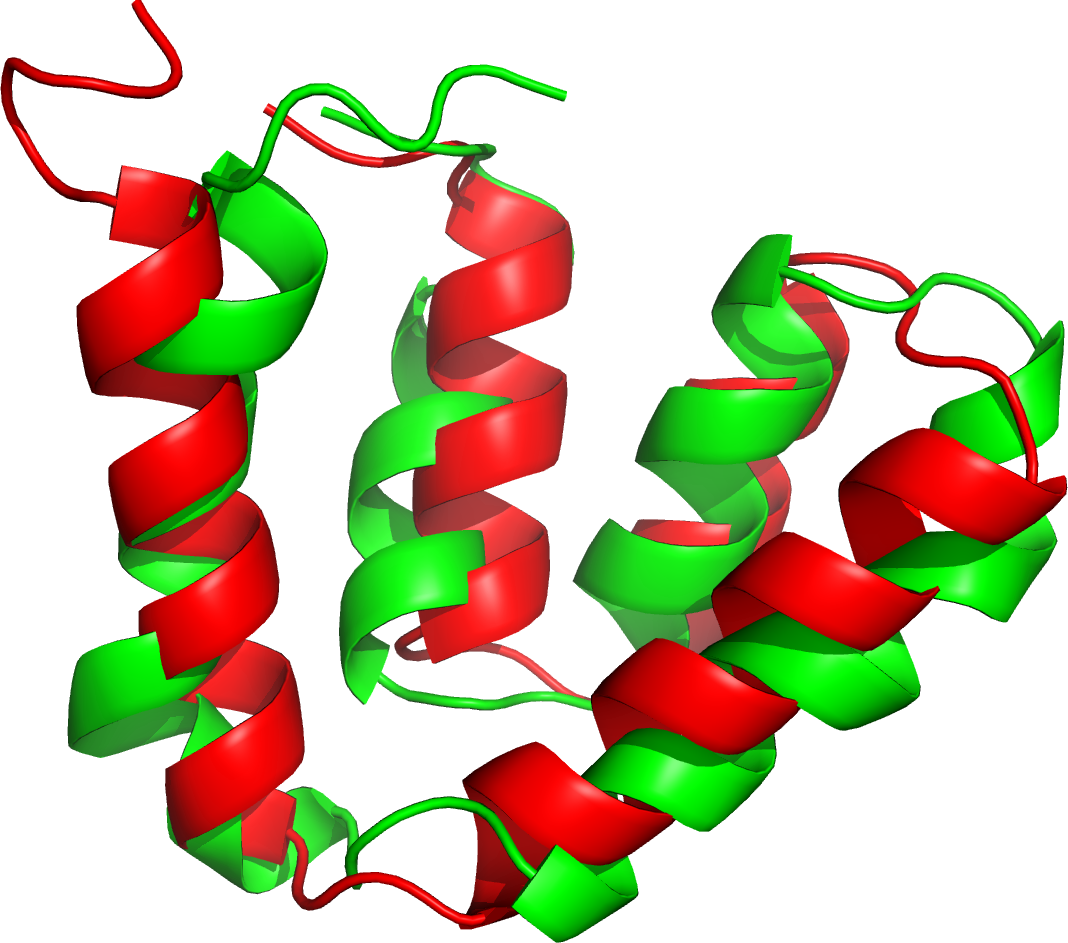
\includegraphics[width=0.9\linewidth]{Figuras/prots/1utg_render.png}
    \caption{1utg (4.41\AA)}
    \label{fig:1utg-conformation}
  \end{subfigure}
% \end{figure}
% \begin{figure}
  \begin{subfigure}{0.32\linewidth}
    \centering
    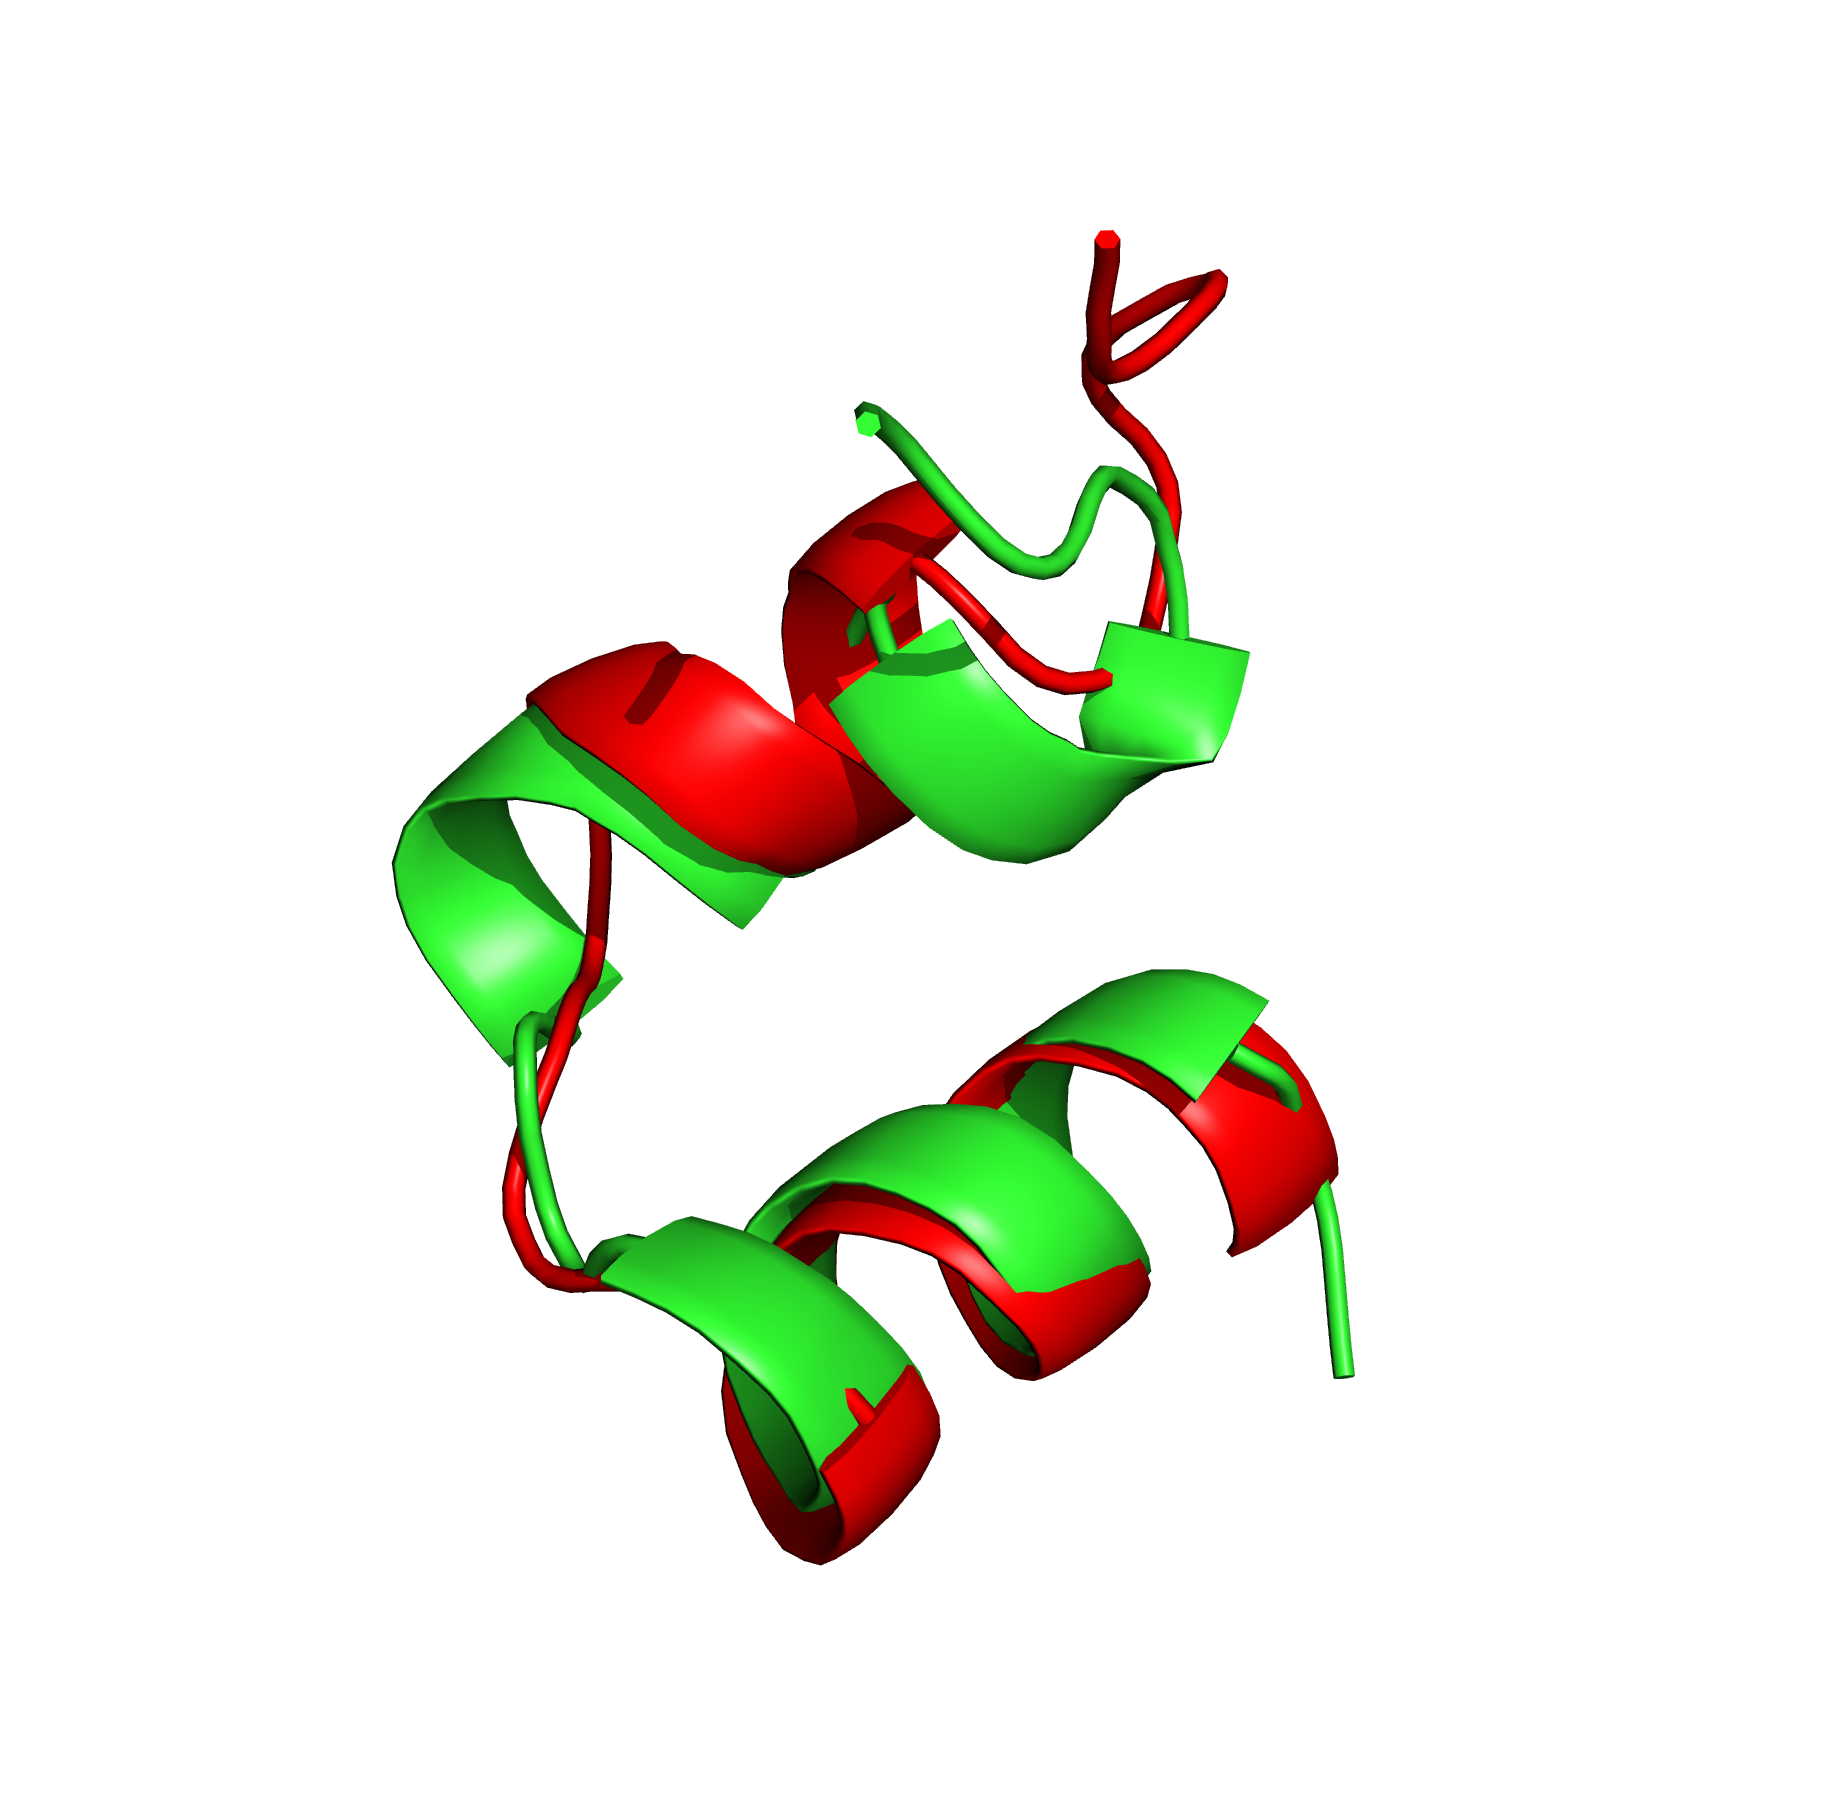
\includegraphics[width=0.9\linewidth]{Figuras/prots/1wqc_render.png}
    \caption{1wqc (2.15\AA)}
    \label{fig:1wqc-conformation}
  \end{subfigure}
%
  \begin{subfigure}{0.32\linewidth}
    \centering
    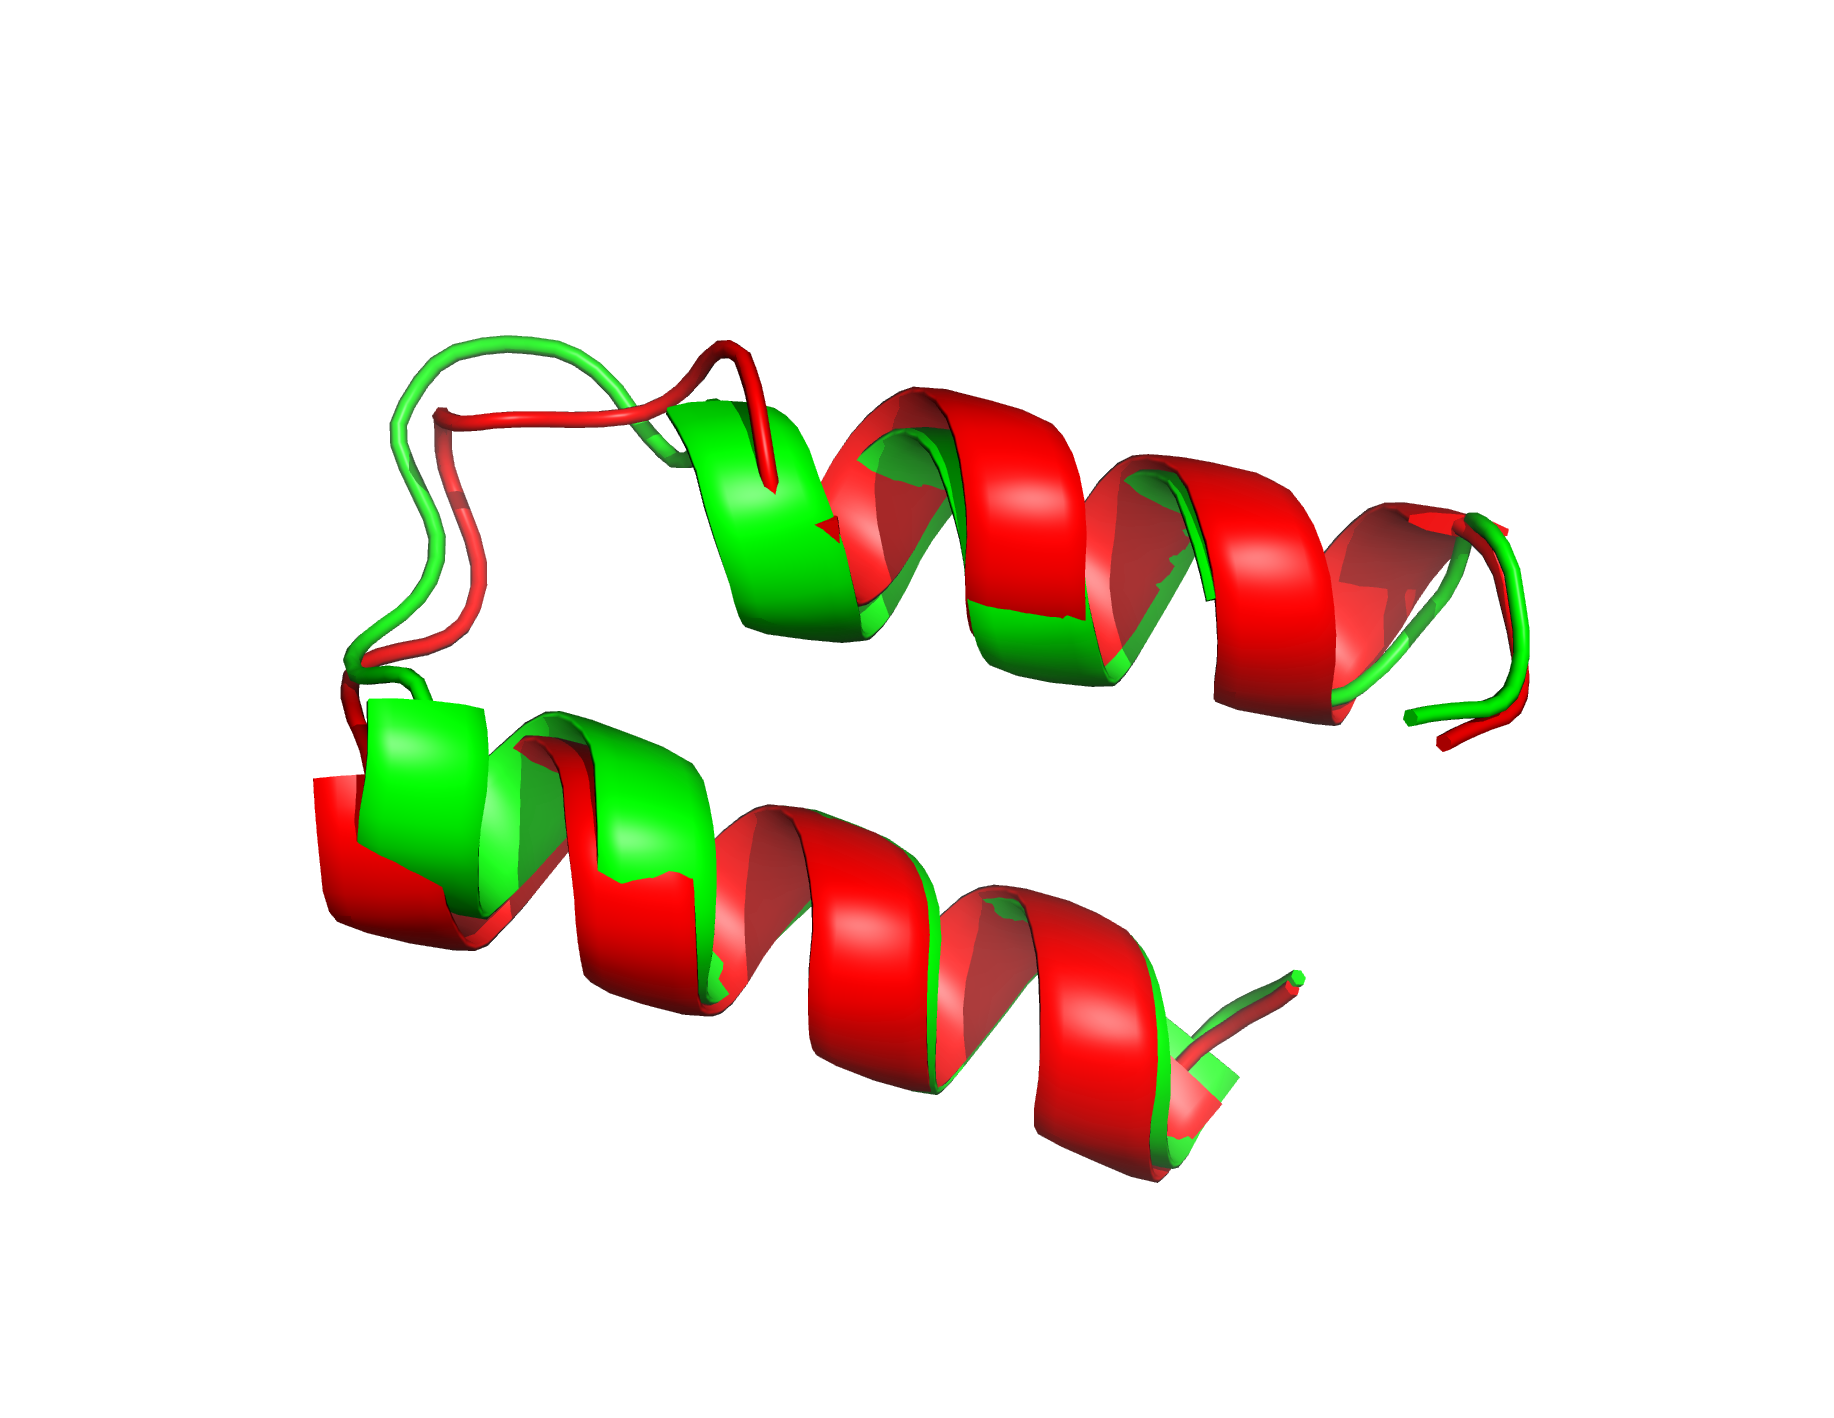
\includegraphics[width=0.9\linewidth]{Figuras/prots/1zdd_render.png}
    \caption{1zdd (1.07\AA)}
    \label{fig:1zdd-conformation}
  \end{subfigure}
%
  \begin{subfigure}{0.32\linewidth}
    \centering
    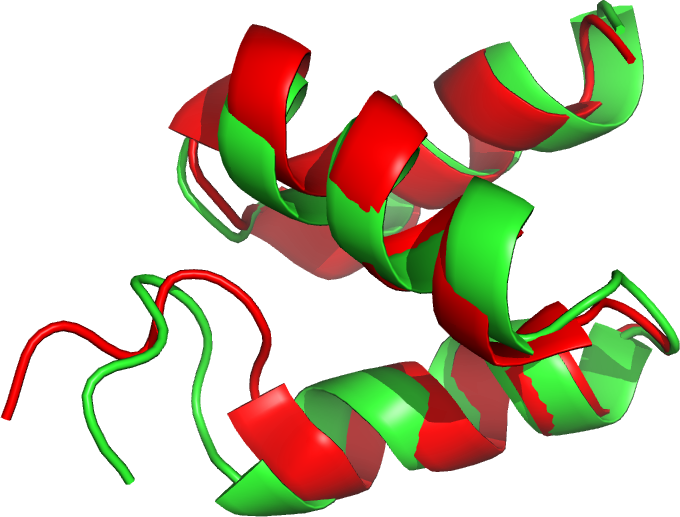
\includegraphics[width=0.9\linewidth]{Figuras/prots/2mr9_render.png}
    \caption{2mr9 (1.66\AA)}
    \label{fig:2mr9-conformation}
  \end{subfigure}
  \caption{The predicted conformations (in green/light gray) compared to the
  native conformation (in red/darker gray). The RMSD between the predicted and
  native conformation is show between parenthesis.}
  \label{fig:all-conformations}
\end{figure}


In Figure~\ref{fig:all-conformations} all conformations from the 10 best
predictions measured by RMSD from ppf-mc are presented. The proteins are presented in
lexicographical order. The predicted conformation is presented in green and the
native conformation is presented in red\footnote{For the readers with a black
and white copy, the predicted conformation is in a light shade of grey, while
the native conformation is in dark grey.}.

Proteins 1enh, 1rop, 1utg, 1wqc, 1zdd and 2mr9 had near native conformations.
%There is very little to comment for these particular predictions.
All the secondary structures are present in their respective regions and the
coil sections closely match their native counterparts.
For protein 1acw,
which had a relatively high RMSD, considering the size of the protein, there are
two main prediction errors. Firstly, the $\beta$-sheets did not form, and, where
should be one, there is an $\alpha$ helix instead. The second error, is that the
$\alpha$ helix is in the wrong place and split. It starts where it should,
however, it only has a single turn. A second helix forms at the eighth residue
and goes on for ten more residues. Both these errors can be traced down to an
error in the Secondary Structure Prediction, which the proposed methods have no
way to avoid. For 1ail, the prediction is mostly correct, however, two helices
are split apart. The first, to the left of the image, and the second, in the
middle helix. These errors were prediction failures that occurred in the proposed methods.
This protein in particular has a correct secondary structure as an starting
point.

On 1crn, a relatively complex protein, has an overall correct fold. The fine
details, however, are lacking. The two helices are mostly missing and the
sheets did not fold. These two errors can be traced down to the secondary
structure prediction used as input. For 1l2y a similar scenario occurs, where
the main source of error is in the data fed to the prediction engine. The
overall shape of the protein was correctly predicted. The helix is completely
missing.

Interestingly, on 4 of the proteins with the biggest visually detectable error
(1acw, 1ail, 1crn and 1l2y)
3 of them (1acw, 1crn and 1l2y) had its source of error outside to the prediction. The proposed method
relies heavily on the predicted secondary structure, and as such, has to deal
with uncertainty. In only a single case the major error in a prediction was
generated during the prediction itself, as occurred on 1ail.
